\documentclass[12pt,a4paper]{article}

\usepackage[utf8]{inputenc}
\usepackage[ngerman]{babel}
\usepackage[T1]{fontenc}
\usepackage{amsmath}
\usepackage{amsfonts}
\usepackage{amssymb}
\usepackage{graphicx}
\usepackage[left=2cm,right=2cm,top=2cm,bottom=3cm]{geometry}
\usepackage{multicol}
\usepackage{booktabs}
\usepackage[hidelinks]{hyperref}
\usepackage{tikz}
\usepackage{pgfplots}
\usepackage{blindtext}
\usepackage{array}
\usepackage{multirow}
\usepackage{bigdelim}
\usepackage{colortbl}
\usepackage{fancyhdr} 
\usepackage{tabularx}
\usepackage{xcolor}
\usepackage{color}
\usetikzlibrary{decorations.text}
\usetikzlibrary{tikzmark}
\pagestyle{fancy} 
	\fancyhf{} 
	\fancyhead[L]{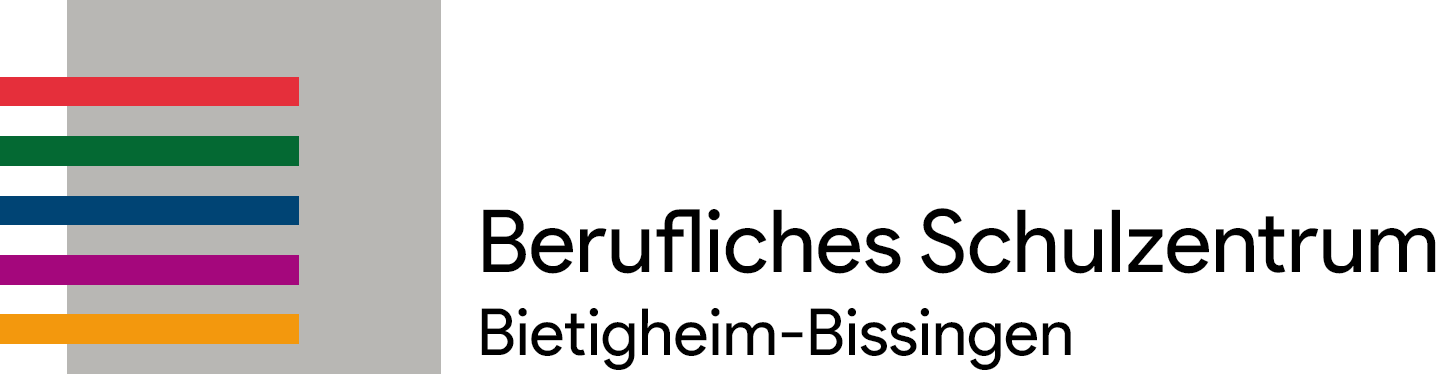
\includegraphics[scale=0.15]{Bilder/BSZLOGO.png}} 
	\fancyhead[C]{\slshape Informationstechnik} 
	\fancyhead[R]{\slshape ABI Zusammenfassung}
	\fancyfoot[C]{\thepage}

\usepackage{helvet}
\renewcommand{\familydefault}{\sfdefault}

\author{\slshape Jannis Müller, Robin Rausch}
\title{IT ABI Zusammenfassung}
\date{\slshape 03 April 2021}
\begin{document}
\maketitle
\tableofcontents
\newpage

\section{Zahlensysteme}
	\begin{minipage}{.49\textwidth}
	
	\subsection{Dezimalsystem}
		\begin{tabularx}{9cm}{XX}
            Nennwerte:&0,1,[\dots],8,9\\
            Basis:&10\\
            Größter Nennwert:&9\\
        \end{tabularx}\newline
        \begin{center}
        	\footnotesize
            \begin{tabular}{|c|c|}
                \hline

                $10^1$ & $10^0$ \\
                \hline
                10     & 1      \\
                \hline
                \hline
                0      & 0      \\
                0      & 1      \\
                0      & 2      \\
                0      & 3      \\
                0      & 4      \\
                0      & 5      \\
                0      & 6      \\
                0      & 7      \\
                0      & 8      \\
                0      & 9      \\
                1      & 0      \\
                1      & 1      \\
                1      & 2      \\
                1      & 3      \\
                1      & 4      \\
                1      & 5      \\
                \hline
            \end{tabular}
        \end{center}
    \end{minipage}
        \begin{minipage}{.49\textwidth}

    \subsection{Dualsystem}
        \begin{tabularx}{10cm}{XX}
            Nennwerte:&0,1\\
            Basis:&2\\
            Größter Nennwert:&1\\
        \end{tabularx}
        \begin{center}
        	\footnotesize
            \begin{tabular}{|c|c|c|c|}
                \hline

                $2^3$ & $2^2$ & $2^1$ & $2^0$ \\
                \hline
                8     & 4     & 2     & 1     \\
                \hline
                \hline
                0     & 0     & 0     & 0     \\
                0     & 0     & 0     & 1     \\
                0     & 0     & 1     & 0     \\
                0     & 0     & 1     & 1     \\
                0     & 1     & 0     & 0     \\
                0     & 1     & 0     & 1     \\
                0     & 1     & 1     & 0     \\
                0     & 1     & 1     & 1     \\
                1     & 0     & 0     & 0     \\
                1     & 0     & 0     & 1     \\
                1     & 0     & 1     & 0     \\
                1     & 0     & 1     & 1     \\
                1     & 1     & 0     & 0     \\
                1     & 1     & 0     & 1     \\
                1     & 1     & 1     & 0     \\
                1     & 1     & 1     & 1     \\
                \hline
            \end{tabular}
        \end{center}
    \end{minipage}\newline
    \begin{minipage}{.49\textwidth}
        \vspace{0.5cm}
    
        \subsection{Oktalsystem}
            \begin{tabularx}{9cm}{XX}
                Nennwerte:&0,1,[\dots],6,7\\
                Basis:&8\\
                Größter Nennwert:&7\\
            \end{tabularx}
            \begin{center}
            	\footnotesize
                \begin{tabular}{|c|c|}
                    \hline

                    $8^1$ & $8^0$ \\
                    \hline
                    8     & 1      \\
                    \hline
                    \hline
                    0      & 0      \\
                    0      & 1      \\
                    0      & 2      \\
                    0      & 3      \\
                    0      & 4      \\
                    0      & 5      \\
                    0      & 6      \\
                    0      & 7      \\
                    1      & 0      \\
                    1      & 1      \\
                    1      & 2      \\
                    1      & 3      \\
                    1      & 4      \\
                    1      & 5      \\
                    1      & 6      \\
                    1      & 7      \\
                    \hline
                \end{tabular}
            \end{center}
    \end{minipage}
    \begin{minipage}{.49\textwidth}
        \vspace{0.5cm}
        
        \subsection{Hexadezimalsystem}
            \begin{tabularx}{9cm}{XX}
                Nennwerte:&0,1,[\dots],8,9,A,B,C,D,E,F\\
                Basis:&16\\
                Größter Nennwert:&F\\
            \end{tabularx}
            \begin{center}
            	\footnotesize
                \begin{tabular}{|c|c|}
                    \hline

                    $16^1$ & $16^0$ \\
                    \hline
                    8     & 1      \\
                    \hline
                    \hline
                    0      & 0      \\
                    0      & 1      \\
                    0      & 2      \\
                    0      & 3      \\
                    0      & 4      \\
                    0      & 5      \\
                    0      & 6      \\
                    0      & 7      \\
                    0      & 8      \\
                    0      & 9      \\
                    0      & A      \\
                    0      & B      \\
                    0      & C      \\
                    0      & D      \\
                    0      & E      \\
                    0      & F      \\
                    \hline
                \end{tabular}
            \end{center}
    \end{minipage}

\section{Aufbau Computer}

\subsection{Von Neumann Prinzip}
	\textbf{Quellcode:}
    \begin{align*}
        \text{zahl1} &= \text{1}; \\
        \text{zahl2} &= \text{4}; \\
        \text{zahl1 + zahl2} &= \text{sum};
    \end{align*}
    \vspace{-1cm}
	\begin{figure}[h]
    	\centering
    	\begin{tikzpicture}
        	\draw[black, very thick] (-4,-4) rectangle (2,8);
        	\node (A) at (-1, 7.4){\textbf{CPU}};
        	\draw[black, very thick](-4,6.8) -- (2,6.8);
        	\draw[black, very thick, dotted](-4,0) -- (2,0);
        	\node (B) at (10, 7.4) {\textbf{Arbeitsspeicher}};
        	\draw[black, very thick](8,-4) -- (8,8);
        	\draw[black, very thick](12,-4) -- (12,8);
        	\draw[black, very thick](8,6.8) -- (12,6.8);
        	\draw[black, very thick](8,5) -- (12,5);
        	\draw[black, very thick](8,3.2) -- (12,3.2);
        	\draw[black, very thick](8,1.4) -- (12,1.4);
        	\draw[black, very thick](8,-0.4) -- (12,-0.4);
        	\draw[black, very thick](8,-2.2) -- (12,-2.2);
        	\node (C) at (-1, 4.4) {Steuerwerk};
        	\node (D) at (-1, 3.4) {Rechenwerk};
        	\node (E) at (-1, 2.4) {Arithemtic Logical Unit(ALU)};
        	\node (F) at (-1, -1.4) {Speicherwerk};
        	\node (G) at (-1, -2.6) {Ein- und Ausgabewerk};
        	\node (I) at (10, 5.9) {5};
        	\node (J) at (10, 4.1) {\textcolor{orange}{9}};
        	\node (K) at (10, 2.3) {4};
        	\node (L) at (6.5, 6.8) {\underline{Adresse:}};
        	\node (M) at (6.5, 5.9) {\textit{zahl1}};
        	\node (N) at (6.5, 4.1) {\textcolor{orange}{\textit{sum}}};
        	\node (O) at (6.5, 2.3) {\textit{zahl2}};
        	\draw[->, very thick] (M) to[out=200, in=-30] (G);
        	\draw[->, very thick] (O) to[out=200, in=-30] (G);
        	\draw[->, very thick, dotted, blue] (G) to[out=160, in=200] (D);
        	\draw[->, very thick, orange] (D) to[out=-30, in=160] (N);
    	\end{tikzpicture}
    	\caption{Von Neumann Prinzip}
	\end{figure}\newpage

\section{Betriebssysteme}
	\begin{figure}[h]
		\centering
        \begin{tikzpicture}
            \def\Radius{2}
            \def\radius{1}
            \begin{scope}[even odd rule]
                \clip[rotate=0.0] (0,0) -- (0:\Radius) arc (0:360:\Radius) --cycle;
                \fill[cyan!60!white] circle[radius=\Radius] circle[radius=\radius];
                \pgfmathsetmacro\bradius{(\radius+\Radius-(\ht\strutbox-\dp\strutbox)/(1cm))/2}
                \path[decoration={text along path,text align={align=center},reverse path,text={Prozess und 								Speicherverwaltung}}, decorate,rotate=-50] (0:\bradius) arc (0:280:\bradius);
            \end{scope}
            \def\Radius{3}
            \def\radius{2}
            \begin{scope}[even odd rule]
                \clip[rotate=0.0] (0,0) -- (0:\Radius) arc (0:360:\Radius) --cycle;
                \fill[cyan!40!white] circle[radius=\Radius] circle[radius=\radius];
                \pgfmathsetmacro\bradius{(\radius+\Radius-(\ht\strutbox-\dp\strutbox)/(1cm))/2}
                \path[
                decoration={text along path,text align={align=center},reverse path,
                text={Kernel}},
                decorate,rotate=-50]
                (0:\bradius) arc (0:280:\bradius);
            \end{scope}
            \def\Radius{4}
            \def\radius{3}
            \begin{scope}[even odd rule]
                \clip[rotate=0.0] (0,0) -- (0:\Radius) arc (0:360:\Radius) --cycle;
                \fill[cyan!20!white] circle[radius=\Radius] circle[radius=\radius];
                \pgfmathsetmacro\bradius{(\radius+\Radius-(\ht\strutbox-\dp\strutbox)/(1cm))/2}
                \path[
                decoration={text along path,text align={align=center},reverse path,
                text={Anwendersoftware}},
                decorate,rotate=-50]
                (0:\bradius) arc (0:280:\bradius);
            \end{scope}
            \draw [line width = 1.5pt](0,0)circle(2);
            \draw [line width = 1.5pt](0,0)circle(3);
            \draw [line width = 1.5pt](0,0)circle(4);
            \filldraw[fill=cyan!80!white, draw=black, line width = 1.5pt](0,0) circle (1);
            \node at (0,0){\small Hardware};
        \end{tikzpicture}
        \caption{Aufbau eines Betriebssystemes}
	\end{figure}

\subsection{Kernel}
    Der Kernel ist die Schnittstelle zwischen der Anwendersoftware und der Speicher- und Prozessverwaltung. Er kann auch als Betriebssystem-Kern bezeichnet werden.

\subsubsection{Monolithischer Kernel}
	\begin{description}
    	\item[+]{sehr schnell, da alles im Kernel geschieht und es kaum Schnittstellen hat}
    	\item[-]{wenn eine Komponente defekt ist oder einen Fehler hat, ist der Kernel nichtmehr \\ funktionsfähig}
    	\item[-]{Updates müssen im Gesamten direkt erfolgen(z.B. Treiberupdates)}
	\end{description}
    Der Monolitische Kernel wird bei Betriebsystemen wie z.B. DOS, Linux und Android verwendet.

\subsubsection{Mirkokernel}
	\begin{description}
    	\item[+]{wenn eine Komponente defekt ist oder einen Fehler hat, kann man den Kernel trotzdem weiterhin 							 verwenden}
    	\item[-]{Prozesse dauern länger, da auch Prozesse/Treiber ausgelagert sind}
	\end{description}
    Der Mirkokernel wird bei Betriebsystemen wie z.B. Echtzeitsbetriebssystemen oder RISC OS verwendet.

\subsubsection{Hybridkernel}
	\begin{description}
    	\item[+]{Nutzung beider Vorteile}
    	\item[-]{Nutzung beider Nachteile}
	\end{description}
    Der Hybridkernel wird bei Betriebsystemen wie z.B. Windows oder MAC OS verwendet.

\subsection{Master Boot Record (MBR)}
    Der Master Boot Record (kurz MBR) enthält ein Startprogramm für BIOS-basierte Computer und eine Partitionstabelle.
    Außerdem werden durch den MBR die Partitionen einer Festplatte eingeteilt. Zudem kann man die Betriebssysteme und Dateisysteme der einzelnen Partitionen herauslesen.
	\begin{table}[h]
		\renewcommand{\arraystretch}{1.5}
		\caption{Partitionstabelleneinträge}
		\vspace{.2cm}
        \begin{tabularx}{\columnwidth}{|c|X|}
            \hline
            Adresse&Inhalt \\
            \hline
            00&80hex = bootfähige Partition \\
            &00hex = nicht bootfähige Partition \\
            \hline
            01&CHS-Eintrag des ersten Sektors \\
            \hline
            04&Typ der Partition (Dateisystem/Partitionsytp) \\
            \hline
            05&CHS-Eintrag des letzten Sektors \\
            \hline
            08&Startsektor nach LBA\\
            \hline
            0C&Anzahl der Sektoren in der Partition \\
            \hline
        \end{tabularx}
	\end{table}
    \begin{table}[h]
	\caption{Master Boot Record}
	\vspace{.2cm}
    \begin{tabularx}{\columnwidth}{|l|X|X|X|X|X|X|X|X|X|X|X|X|X|X|X|X|X|}
        \hline
        \rowcolor{yellow}Offset&0&1&2&3&4&5&6&7&8&9&A&B&C&D&E&F \\
        \hline
        \rowcolor{yellow}0000&eb&48&90&10&8e&d0&bc&00&b0&b8&00&00&8e&d8&8e&c0 \\
        \hline
        \rowcolor{yellow}0010&fb&be&00&7c&bf&00&06&b9&00&02&f3&a4&ea&21&06&00 \\
        \hline
        \multicolumn{17}{|c|}{\dots}\\
        \hline
        \rowcolor{yellow}01a0&10&ac&3c&00&75&f4&c3&00&00&00&00&00&00&00&00&00 \\
        \hline
        \cellcolor{yellow}01b0&\cellcolor{yellow}00&\cellcolor{yellow}00&\cellcolor{yellow}00&\cellcolor{yellow}				00&\cellcolor{yellow}00&\cellcolor{yellow}00&\cellcolor{yellow}00&\cellcolor{yellow}00&\cellcolor{green!				70!blue}00&\cellcolor{green!70!blue}00&\cellcolor{green!70!blue}00&\cellcolor{green!70!blue}00&							\cellcolor{cyan!60!white}00&\cellcolor{cyan!60!white}00&\cellcolor{red!60!white}80&\cellcolor{red!60!					white}01 \\
        \hline
        \rowcolor{red!60!white}01c0&01&00&83&fe&ff&ff&3f&00&00&00&41&29&54&02&\cellcolor{red!50!white}00&						\cellcolor{red!50!white}fe\\
        \hline
        \rowcolor{red!50!white}01d0&ff&ff&82&fe&ff&ff&80&29&54&02&fa&e7&1d&00&\cellcolor{red!40!white}00&						\cellcolor{red!40!white}fe \\
        \hline
        \rowcolor{red!40!white}01e0&ff&ff&83&fe&ff&ff&7a&11&72&02&fa&e7&1d&00&\cellcolor{red!30!white}00&						\cellcolor{red!30!white}fe \\
        \hline
        \rowcolor{red!30!white}01f0&ff&ff&05&fe&ff&ff&74&f9&8f&02&0c&83&6c&04&\cellcolor{purple!50!blue}55&						\cellcolor{purple!50!blue}aa \\
        \hline
    \end{tabularx}
	\textcolor{white}{Abstandhalter}\newline
	\begin{tabularx}{\columnwidth}{XXXXX}
		\cellcolor{yellow}&\cellcolor{green!70!blue}&\cellcolor{cyan!60!white}&\cellcolor{red!60!white}&						\cellcolor{purple!50!blue} \\
		Bootloader&Disk Signatur&Nullbytes&Partitionstabelle&Magic Number \\
	\end{tabularx}
\end{table}

\subsection{GPT}
    Die Guide Partition Table ist der bessere MBR und hat folgende Vor- und Nachteile gegenüber dem MBR:
	\begin{description}
    	\item[+]{Funktioniert auch bei 64-Bit Systemen}
    	\item[+]{beliebig viele primäre Partitionen}
    	\item[+]{verfügt über Schutz- und Sicherheitsmerkmale(Backups \& Prüfsummen)}
    	\item[-]{Nur mit UEFI kompatibel}
	\end{description}

\subsection{UEFI und BIOS}
    UEFI ist das modernere und bessere BIOS. UEFI verfügt gegenüber BIOS folgende Vorteile:
	\begin{itemize}
    	\item schnelleres Starten durch paralleles Laden der Treiber
    	\item Datenträger können auch mit mehr als 2TB booten
    	\item Funktioniert auch bei modernen 64-Bit Systemen
    	\item Netzwerke können auch gebootet werden
	\end{itemize}

\section{Dateisysteme}

\subsection{FAT}
    Die FAT (\textit{File Allocation Table, Dateizuordnungstabelle}) stellt ein Inhaltsverzeichnis der Festplatte dar und ist notwendig, um die auf dem Datenträger bereitstehenden Daten zu finden. In einem 16-Bit System (FAT 16) sind genau $2^{16} = 65536$ Adressenverwaltungseinträge in der FAT möglich. Bei einer Clustergröße von 512 Byte beträgt die maximale Partitionsgröße 32 MiB ($2^{16} \cdot 512 \text{ Byte}$).
	\begin{figure}[h]
        \centering
        \begin{tikzpicture}
            \fill [olive!40!white](-6,0)rectangle(-4.5,-3);
            \fill [cyan!80!white](-4.5,-1.5)rectangle(0.75,-3);
            \fill [cyan!60!white](-4.5,0)rectangle(-3,-1.5);
            \fill [cyan!40!white](-3,0)rectangle(-1.5,-1.5);
            \fill [cyan!20!white](-1.5,0)rectangle(0.75,-1.5);
            \fill [purple!80!white](0.75,-1.5)rectangle(6,-3);
            \fill [purple!60!white](0.75,-0)rectangle(2.75,-1.5);
            \fill [purple!40!white](2.75,-0)rectangle(4.75,-1.5);
            \fill [purple!20!white](4.75,-0)rectangle(6,-1.5);
            \node at (-5.25,-0.4){Boot};
            \node at (-5.25,-1){Block};
            \node at (-5.25,-1.9){Boot};
            \node at (-5.25,-2.5){Progr.};
            \node at (-2,-2.25){Systembereich};
            \node at (3.25,-2.25){Datenbereich};
            \node at (-3.75,-0.75){FAT};
            \node at (-2.25,-0.5){FAT};
            \node at (-2.25,-1){Kopie};
            \node at (-0.4,-0.5){Root};
            \node at (-0.4,-1){Directory};
            \node at (1.75,-0.75){Cluster 1};
            \node at (3.75,-0.75){Cluster 2};
            \node at (5.375,-0.75){\dots};
            \draw [line width = 1.2pt] (-6,0)rectangle(6,-3);
            \draw [line width = 1.2pt] (-6,-1.5)--(6,-1.5);
            \draw [line width = 1.2pt] (-4.5,0)--(-4.5,-3);
            \draw [line width = 1.2pt] (0.75,0)--(0.75,-3);
            \draw [line width = 1.2pt] (-3,0)--(-3,-1.5);
            \draw [line width = 1.2pt] (-1.5,0)--(-1.5,-1.5);
            \draw [line width = 1.2pt] (2.75,0)--(2.75,-1.5);
            \draw [line width = 1.2pt] (4.75,0)--(4.75,-1.5);
        \end{tikzpicture}
        \caption{Aufbau des FAT Dateisystems}
	\end{figure}\newline
    Durch die geringe Clustergröße können Dateien meist nur fragmentiert abgelegt werden. In einer Dateizuordnungstabelle werden Dateipfade gespeichert und können ausgelesen werden. Das richtige Zusammensetzen der Fragmente ist so möglich.\\
    Ein Nachteil des FAT Systemes liegt darin, dass die FAT an einer festen Position auf dem Datenträger gespeichert ist. Bei Festplatten (Speichermedien mit rotierender Disk und Lesekopf) muss der Lesekopf bei jedem Lese/Schreib Vorgang zur FAT und zurück bewegt werden. Dann muss gewartet werden, bis die FAT den Lesekopf passiert. Das kostet viel Zeit. Heutzutage findet man das FAT System in der Flash Drive Technik.

\subsection{NTFS}
    Das NTFS (\textit{New Technology File System}) Dateisystem wurde erstmals mit Windows NT (\textit{New Technology}) eingeführt und ist seither das preferierte Dateisystem von Windows. NTFS verwaltet Dateien anders als bei FAT in der MFT (\textit{Mater File Table}). Diese enthält die sogenannten Records. Zu jeder abgelegten Datei existiert also ein Record in der MFT der folgende Informationen enthält: Header, Informationen (z.B. Erstellungsdatum), den Dateinamen, Zugriffsrechte und die eigentlichen Daten bzw. die Position der Daten im Datenbereich. Dateien kleiner 1.5 KiB können direkt in den Record in der MFT gespeichert werden, wohingegen Dateien größer 1.5 KiB in den Datenbereich des Datenträgers gespeichert werden. Der Record verweist dann auf die entsprechende Stelle. Der Datenbereich ist bei NTFS variabel. Daraus resultieren kürzere Lese/Schreib Zeiten. Außerdem ist die MFT zwei mal zwischen den Datenbereichen enthalten.
    \begin{figure}[h]
        \centering
        \begin{tikzpicture}
            \fill [olive!40!white](-7,0)rectangle(-3,-4);
            \fill [purple!80!white](-3,0)rectangle(-1,-4);
            \fill [cyan!60!white](-1,0)rectangle(1,-4);
            \fill [purple!60!white](1,0)rectangle(3,-4);
            \fill [cyan!40!white](3,0)rectangle(5,-4);
            \fill [purple!40!white](5,0)rectangle(7,-4);
            \draw [line width = 1.2pt](-7,0)rectangle(7,-4);
            \draw [line width = 1.2pt](-7,-1)--(-3,-1);
            \draw [line width = 1.2pt](-5,-1)--(-5,-4);
            \draw [line width = 1.2pt](-3,0)--(-3,-4);
            \draw [line width = 1.2pt](-1,0)--(-1,-4);
            \draw [line width = 1.2pt](1,0)--(1,-4);
            \draw [line width = 1.2pt](3,0)--(3,-4);
            \draw [line width = 1.2pt](5,0)--(5,-4);
            \node at (-5,-0.5){Boot-Block};
            \node [rotate=90] at (-6,-2.5){BIOS Block};
            \node [rotate=90] at (-4,-2.5){Viewers MFT};
            \node [rotate=90] at (-2,-2){Variabler Bereich};
            \node [rotate=90] at (0,-2){MFT};
            \node [rotate=90] at (2,-2){Variabler Bereich};
            \node [rotate=90] at (4,-2){MFT};
            \node [rotate=90] at (6,-2){Variabler Bereich};
        \end{tikzpicture}
        \caption{Aufbau einer NTFS Partition}
	\end{figure}
	\begin{figure}[h]
        \centering
        \begin{tikzpicture}
            \fill [cyan!60!white] (-7,0)rectangle(1,-4);
            \fill [purple!60!white] (1,0)rectangle(7,-4);
            \draw [line width = 1.2pt](-7,0)rectangle(7,-4);
            \draw [line width = 1.2pt](-5,0)--(-5,-4);
            \draw [line width = 1.2pt](-3,0)--(-3,-4);
            \draw [line width = 1.2pt](-1,0)--(-1,-4);
            \draw [line width = 1.2pt](1,0)--(1,-4);
            \node [rotate=90] at (-6,-2){Header};
            \node [rotate=90] at (-4,-2){Informationen};
            \node [rotate=90] at (-2,-2){Dateiname};
            \node [rotate=90] at (0,-2){Rechte};
            \node [rotate=90] at (2,-2){Daten};
        \end{tikzpicture}
        \caption{NTFS Record Dateien kleiner 1.5KiB}
        \end{figure}
        \begin{figure}[h]
        \centering
        \begin{tikzpicture}
            \fill [cyan!60!white] (-7,0)rectangle(1,-4);
            \fill [purple!60!white] (1,0)rectangle(7,-4);
            \draw [line width = 1.2pt](-7,0)rectangle(7,-4);
            \draw [line width = 1.2pt](-5,0)--(-5,-4);
            \draw [line width = 1.2pt](-3,0)--(-3,-4);
            \draw [line width = 1.2pt](-1,0)--(-1,-4);
            \draw [line width = 1.2pt](1,0)--(1,-4);
            \node [rotate=90] at (-6,-2){Header};
            \node [rotate=90] at (-4,-2){Informationen};
            \node [rotate=90] at (-2,-2){Dateiname};
            \node [rotate=90] at (0,-2){Rechte};
            \filldraw [fill=white,line width = 1.2pt](1.2,-0.2)rectangle(6.8,-3.8);
            \fill [purple!20!white] (1.2,-0.2)rectangle(6.8,-1.1);
            \draw [line width = 1.2pt](1.2,-1.1)--(6.8,-1.1);
            \draw [line width = 1.2pt](1.2,-2)--(6.8,-2);
            \draw [line width = 1.2pt](1.2,-2.9)--(6.8,-2.9);
            \draw [line width = 1.2pt](3,-0.2)--(3,-3.8);
            \draw [line width = 1.2pt](4.8,-0.2)--(4.8,-3.8);
            \node at (2.1,-0.7){VCN};
            \node at (3.9,-0.7){LCN};
            \node at (5.8,-0.7){Größe};
        \end{tikzpicture}
        \caption{NTFS Record Dateien größer 1.5KiB}
	\end{figure}\newpage
    \noindent NTFS verfügt über eine hohe Fehlertoleranz. Eine geschriebene Datei wird mit der sich noch im RAM befindender Original Datei verglichen, um Fehler zu vermeiden. Wird ein Fehler erkannt, wird der betreffende Block als fehlerhaft markiert. Der Schreibvorgang wird dann an einem Anderen versucht. Dieses Prinzip nennt man Hot-Fixing. NTFS verfügt zudem über eine sogenannte LOGFILE. Alle Transaktionen werden in diese eingetragen. So kann nach einem Absturz verlorenes Datengut wiederhergestellt werden. NTFS Dateinamen können bis zu 255 Unicode Zeichen lang sein. 

\subsubsection{Dataruns}
    Ist ein Dateneintrag bei NTFS zu groß, muss dieser in den Datenbereich ausgelagert werden, liegt eine sehr große Datei vor, so muss diese zusätzlich fragmentiert werden. Diese Fragmentierung wird mit Hilfe des B-Tree Prinzipes in den Datenbereich des Records eingetragen. Mittles LCN-VCN Mapping ist es nun möglich die fragmentierte Datei auf dem Datenträger richtig und vollständig zusammen zu setzen.

\section{Prozessverwaltung}
    Die Betriebsmittel des Computersystems müssen zwischen den verschiedenen laufenden Programmen und Systemaufgaben verteilt werden. Zu diesem Zweck werden die einzelnen Aufgaben als Prozesse ausgeführt, die vom Betriebssystem verwaltet werden.

\subsection{Prozesse}
    Ein Prozess besteht aus dem Programmcode und dem Prozesskontext. Der Prozesskontext wiederum setzt sich zusammen aus den Registerinhalten des Prozessors, Speicherbereichen für die Daten und weiteren Betriebsmitteln.\newline
    Ein Programm kann sich aus mehreren Prozessen (Windows: Tasks) zusammensetzen. Ein Prozess kann Unterprozesse besitzen. So ist hier B ein Unterprozess von A, D E und F wiederum sind Unterprozesse von B.
    \begin{figure}[h]
    \centering
        \begin{tikzpicture}
            \filldraw[fill=cyan!60!white, line width=1.2pt](0,0)circle(1cm);
            \node at (0,0) {A};
            \filldraw[fill=orange!60!white, line width=1.2pt](-3,-1)circle(1cm);
            \node at (-3,-1) {B};
            \filldraw[fill=purple!80!white, line width=1.2pt](-5,-1)circle(.5cm);
            \node at (-5,-1) {D};
            \filldraw[fill=purple!60!white, line width=1.2pt](-4.3,-2.5)circle(.5cm);
            \node at (-4.3,-2.5) {E};
            \filldraw[fill=purple!40!white, line width=1.2pt](-2.5,-3)circle(.5cm);
            \node at (-2.5,-3) {F};
            \filldraw[fill=olive!30!cyan, line width=1.2pt](4,-1.5)circle(2cm);
            \node at (5,-0.5) {C};
            \filldraw[fill=olive!20!cyan, line width=1.2pt](3.2,-1)circle(0.85cm);
            \node at (3.2,-1) {Thread1};
            \filldraw[fill=olive!20!cyan, line width=1.2pt](4.5,-2.3)circle(0.85cm);
            \node at (4.5,-2.3) {Thread2};
            \draw [line width=1.5pt] (-0.88,-0.5)--(-2.02,-0.9);
            \draw [line width=1.5pt] (0.88,-0.5)--(2.1,-0.9);
            \draw [line width=1.5pt] (-4.5,-1)--(-4,-1);
            \draw [line width=1.5pt] (-3.6,-1.8)--(-3.95,-2.15);
            \draw [line width=1.5pt] (-2.75,-2)--(-2.6,-2.5);
            \end{tikzpicture}
            \caption{Prozesse, Unterprozesse und Threads}
    \end{figure}

\subsubsection{Threads}
Prozesse können neben eigenständigen Unterprozessen auch noch Threads haben. Threads sind leichtgewichtige Prozesse innerhalb eines übergeordneten Prozesses. Threads teilen sich mit anderen Threads verschiedene Betriebsmittel. Threads, die dem selben Prozess zugeordnet sind, verwenden den gleichen Adressraum. Dadurch ist eine Kommunikation zwischen diesen Threads möglich.
	\begin{figure}[h]
		\centering
		\begin{tikzpicture}
			\filldraw[fill=olive!30!cyan, line width=1.2pt](4,-1.5)circle(2cm);
            \node at (5,-0.5) {C};
            \filldraw[fill=olive!20!cyan, line width=1.2pt](3.2,-1)circle(0.85cm);
            \node at (3.2,-1) {Thread1};
            \filldraw[fill=olive!20!cyan, line width=1.2pt](4.5,-2.3)circle(0.85cm);
            \node at (4.5,-2.3) {Thread2};
		\end{tikzpicture}
		\caption{Threads in Prozess C}
	\end{figure}
	
\subsubsection{Prozesszustände}
Ein Prozess kann folgende Zustände annehmen:
\begin{figure}[h]
	\centering
	\begin{tikzpicture}
		\filldraw [line width=1.2pt,fill=cyan!60!white] (0,0)circle(1.2cm);
		\node at (0,0){rechnend};
		\filldraw [line width=1.2pt,fill=orange!60!white] (3,-2)circle(1.2cm);
		\node at (3,-2){bereit};
		\filldraw [line width=1.2pt,fill=purple!60!white] (-3,-2)circle(1.2cm);
		\node at (-3,-2){blockiert};
		\draw [<->, line width=1.5pt] (1.1,-0.5)--(2.3,-1);
		\draw [->, line width=1.5pt] (-1.1,-0.5)--(-2.3,-1);
		\draw [->, line width=1.5pt] (-1.7,-2)--(1.7,-2);
	\end{tikzpicture}
	\caption{Prozessmodell}
\end{figure}
	
\subsection{Mehrprozessbetrieb}
Der Kern eines Prozessors kann immer nur einen Prozess bearbeiten. Prozesse nutzen die zur Verfügung stehende Rechenzeit allerdings nicht optimal, da viele Prozesse auf langsamere äußere Einflüsse warten müssen (bsp. Tastatureingabe). Die Wartezeit eines Prozesses kann effizient genutzt werden, indem diese Wartezeit einem anderen Prozess zugeteilt wird. Man unterscheidet hierbei zwischen zwei Prinzipien:
\begin{enumerate}
	\item parallel, wenn jeder Kern einer CPU genau einen Prozess bearbeitet
	\item quasiparallel, wenn ein Kern einer CPU mehrere Prozesse nacheinander bearbeitet.
\end{enumerate}
\begin{minipage}{.45\textwidth}
	\centering
	\begin{tikzpicture}
	\draw [->](0,0)--(4,0);
	\draw [->](0,0)--(0,2);
	\node [rotate=90] at (-0.5,1){Prozesse};
	\node at (2,-0.4){Zeit};
	\filldraw [fill = cyan!60!white] (0.1,0.1)rectangle(3.8,0.7);
	\filldraw [fill = orange!60!white](0.3,0.8)rectangle(3.3,1.4);
	\end{tikzpicture}\newline
	parallel
\end{minipage}
\hspace{1cm}
\begin{minipage}{.45\textwidth}
	\centering
	\begin{tikzpicture}
	\draw [->](0,0)--(4,0);
	\draw [->](0,0)--(0,2);
	\node [rotate=90] at (-0.5,1){Prozesse};
	\node at (2,-0.4){Zeit};
	\filldraw [fill = cyan!60!white] (0.1,0.1)rectangle(1,0.7);
	\filldraw [fill = orange!60!white](1.1,0.1)rectangle(2,0.7);
	\filldraw [fill = purple!60!white](2.1,0.1)rectangle(3,0.7);
	\end{tikzpicture}\newline
	quasiparallel
\end{minipage}

\subsection{Multitasking}
Es wird zwischen zwei Arten von Multitasking unterschieden:
\begin{enumerate}
	\item Koorperatives Multitasking, hier ist es jedem Prozess selbst überlassen, wann er die Kontrolle an das Betriebssystem zurück gibt. Geringer Verwaltungsaufwand, aber es besteht die Gefahr, dass ein unkoorperativer Prozess das System blockiert.
	\item Präemptives Multitasking, hier steuert das Betriebssystem die Vergabe der Rechenzeit. Der Scheduler kann einem Prozess Zeit oder Ereignis gesteuert Rechenzeit entziehen. Somit ist die Bearbeitung wichtigerer Prozesse zu jedem Zeitpunkt möglich, ein unkoorperativer Prozess legt das System nicht lahm. 
\end{enumerate}

\subsubsection{Kontext}
Um einen Prozess unterbrechen zu können, muss dieser nach der Unterbrechung dieselbe Umgebung vorfinden können, welche der Prozess hatte, bevor er unterbrochen wurde. Der Zustand des Prozesses wird also vor der Unterbrechung gespeichert, und bleibt das so lange, bis ihm wieder Rechenzeit zugeteilt wird. Unmittelbar bevor er wieder aktiv wird, wird der gespeicherte Zustand geladen. Aus Sicht des Prozesses scheint es so, als wäre er nie angehalten worden.\newline
Wichtig für dieses Verhalten ist, dass Prozesse abgeschirmt voneinander sein müssen. Prozess A darf den Kontext von Prozess B nicht kennen. Prozess A erfährt immer nur seinen eigenen Kontext.

\subsection{Scheduling}
Konkurrieren mehrere Prozesse um die Rechenzeit, teilt der Scheduler ihnen gemäß folgender Kriterien die Rechenzeit zu:
\begin{enumerate}
	\item \textbf{Fairness}, jeder Prozess erhält einen gerechten Anteil der Rechenzeit
	\item \textbf{Effizienz}, der Prozessor arbeitet möglichst effizient
	\item \textbf{Antwortzeit}, diese wird für interaktiv arbeitende Benutzer minimiert
	\item \textbf{Verweilzeit}, die Wartezeit für die Ausgabe von Stapelaufträgen wird minimiert
	\item \textbf{Durchsatz}, Maximierung der Auftragszahl für ein bestimmtes Zeitintervall
\end{enumerate}

\subsection{Scheduling Strategien}

\subsubsection{First Come First Serve}

\subsubsection{Shortest Job First}

\subsubsection{Round Robin}

\subsubsection{Priority}

\section{Speicherkonzepte}

\subsection{Speicherhierarchie}
    Speicher werden nach ihrer Schnelligkeit in eine Hierarchie eingeordnet, von kurzer zu langer Zugriffszeit.
	\begin{center}
		\begin{tabularx}{13cm}{XXXlXX}
			&&1.& Prozessorregister&&\\
			&&2.& Prozessorcache&&\\
			&&3.& Hauptspeicher&&\\
			&&4.& Festplatte&&\\
			&&5.& Wechseldatenträger&&\\
		\end{tabularx}
	\end{center}

\section{Speicherverwaltung}

\subsection{Direkte Speicherverwaltung}
    Beim Einprogrammbetrieb verwaltet das Betriebssystem den Hauptspeicher als einen großen Speicherblock. Dieser besteht aus System und Benutzerbereich.
    \begin{center}
        \begin{tabularx}{13cm}{|X|X|X|}
            \hline
            Betriebssystem&Programm&freier Speicher \\
            \hline
        \end{tabularx}
    \end{center}
    \textit{Problem:}\newline
    Die Programmgröße ist durch die Speichergröße begrenzt. Der Hauptspeicher ist somit zu klein für alle aktiven Prozesse.\newline
    \textit{Lösung: Swapping}

\subsection{Swapping}
    Beim Swapping wird ein Bereich der Festplatte als sogenannter \textit{'Swap-Space'} deklariert. In diesen können Prozesse ausgelagert werden. Daten und Programmcode des Prozesses werden vollständig in den Swap Space ausgelagert.				
    \begin{center}
	    \textbf{Ein ausgelagerter Prozess kann nicht ausgeführt werden.}
	\end{center}
	\begin{figure}[h]
		\centering
			\begin{tikzpicture}
				\node (A) at (0,2) [circle,draw,fill=purple!45] {Prozess A};
				\node (B) at (0,-0.7) [circle,draw,fill=orange!50] {Prozess B};
				\draw[black, very thick] (-2,-2) rectangle (2,4);
				\node (D) at (0, 3.6){Hauptspeicher};
				\draw[black, very thick] (4.5,-2) rectangle (8.5,4);
				\node (E) at (6.5, 3.6) {Festplatte};
				\node (C) at (6.5,2) [circle,draw,fill=cyan!50] {Prozess C};
				\draw[->, very thick] (A) to[out=10, in=150] (C);
				\draw[->, very thick] (C) to[out=200, in=-30] (A);
				\node (F) at (6.5, -0.7) [circle,draw,fill=blue!30!white] {Prozess D};
				\draw[->, very thick] (B) to[out=10, in=150] (F);
				\draw[->, very thick] (F) to[out=200, in=-30] (B);
				\node (G) at (3.25,1.4){\textcolor{red}{einlagern}};
				\node (H) at (3.25,3.2){\textcolor{red}{auslagern}};
			\end{tikzpicture}
		\end{figure}
	\begin{center}
		Demnach wären hier nur Prozess A und Prozess B ausführbar.
	\end{center}
    \noindent Ein Prozess wird ausgelagert wenn:
	\begin{itemize}
		\item Ein Prozess, der neu entsteht nicht im Hauptspeicher untergebracht werden kann.
		\item Ein Prozess, seinen Hauptspeicherplatz erweitern möchte, jedoch kein zusätzlicher Speicher verfügbar 					  ist.
		\item Ein \textit{wichtigerer} Prozess aus dem Swap-Space eingelagert werden muss und für ihn kein 							  Hauptspeicherbereich verfügbar ist.
	\end{itemize}

\subsection{virtueller Speicher}
    \noindent Festplattenspeicher und Hauptspeicher werden zu einem Speicherblock vereint. Dadurch stehen mehr Speicheradressen zur Verfügung, wie tatsächlich im Hauptspeicher vorhanden sind = virtueller Speicher.
	\begin{center}
		\fcolorbox{green!65!black}{white}{\parbox{\linewidth}{Im Gegensatz zum Swapping können beim virtuellen 								Speicher Prozesse auch nur teilweise im Hauptspeicher stehen, während der Rest meist auf dem 							Festplattenspeicher liegt.}}
	\end{center}
    Jedem Prozess wird ein virtueller Speicher geboten, in den alles außer arbeitenden Code und Daten (bleiben im Hauptspeicher) eingelagert wird. Wird von einem Prozess auf den Speicher zugegriffen, verweist die virtuelle Adresse auf eine reelle Adresse des Hauptspeichers. Dieser Verweis geschieht durch die \textit{MMU (Memory Management Unit)}. Befinden sich die Daten in einem ausgelagerten Festplattenblock, wird dieser in den Hauptspeicher eingelagert. \newline
	\begin{figure}[h]
		\centering
        \begin{tikzpicture}
            \draw[black, very thick, fill=purple!45] (-6,0) rectangle (-1,3);
            \draw[black, very thick] (1,0) rectangle (6,3);
            \draw[black, very thick,fill=orange!50] (-6,-1) rectangle (-1,-4);
            \draw[black, very thick] (1,-1) rectangle (6,-4);
            \node (A) at (-4.9,2.5){Prozess A};
            \node (B) at (-4.9,-1.5){Prozess B};
            \draw[black, very thick,fill=white] (-5.8,0.2) rectangle (-4,2);
            \draw[black, very thick,fill=white] (-3.8,0.2) rectangle (-1.2,2);
            \draw[black, very thick,fill=white] (-5.8,-2) rectangle (-4,-3.8);
            \draw[black, very thick,fill=white] (-3.8,-2) rectangle (-1.2,-3.8);
            \node (C) at (-5,1){Code};
            \node (D) at (-5,-3){Code};
            \node (E) at (-2.5,1.75){virtueller};
            \node (F) at (-2.5,1.3){Speicher};
            \node (G) at (-2.5,-2.25){virtueller};
            \node (H) at (-2.5,-2.7){Speicher};
            \node (I) at (-3,-3.25){$B_1$};
            \node (J) at (-2,-3.25){$B_2$};
            \node (K) at (-3,0.7){$A_1$};
            \node (L) at (-2,0.7){$A_2$};
            \node (M) at (3.5,2.5){Hauptspeicher};
            \node (N) at (3.5,-1.5){Festplatte};
            \draw[black, very thick, fill=orange!50] (1.2,0.2) rectangle (5.8,0.9);
            \draw[black, very thick, fill=purple!45] (1.2,1.2) rectangle (5.8,2);
            \draw[black, very thick,fill=purple!45] (1.2,-2) rectangle (5.8,-2.8);
            \draw[black, very thick,fill=orange!50] (1.2,-3) rectangle (5.8,-3.8);
            \node (O) at (3.5,1.6){Prozess $A_1$};
            \node (P) at (3.5,0.55){Prozess $B_2$};
            \node (Q) at (3.5,-2.45){Prozess $A_2$};
            \node (R) at (3.5,-3.45){Prozess $B_1$};
            \draw [->, very thick, orange](J) to[out=10, in=180] (P);
            \draw [->, very thick, orange](I) to[out=320, in=180] (R);
            \draw [->, very thick, purple](K) to[out=300, in=180] (O);
            \draw [->, very thick, purple](L) to[out=300, in=180] (Q);
            \draw [->, very thick, purple](C) to[out=300, in=180] (K);
            \draw [->, very thick, orange](D) to[out=300, in=180] (I);
            \node (X)  at (6,1.5){};
            \node (Y)  at (6,-2.5){};
            \draw [<->, very thick, red](X) to[out=350, in=10] (Y);
            \node (S) at (6,-0.3)[color=red]{auslagern};
            \node (S) at (6,-0.7)[color=red]{einlagern};
        \end{tikzpicture}
	\end{figure}
    \begin{figure}[h]
	\centering
		\begin{tikzpicture}
            \draw[black, very thick, fill=blue!40!white] (-8,0) rectangle (-4,3);
            \draw[black, very thick] (-2,0) rectangle (2,3);
            \draw[black, very thick] (4,0) rectangle (8,3);
            \node (A) at (-6,2.5){Prozessor};
            \draw[black, very thick, fill=white] (-7.8,1.2) rectangle (-4.2,2);
            \draw[black, very thick, fill=white] (-7.8,0.2) rectangle (-4.2,1);
            \node (B) at (-6,1.6){virtuelle Adresse};
            \node (C) at (-6,0.6){MMU};
            \node (D) at (0,1.5){Hauptspeicher};
            \node (E) at (6,1.5){Festplatte};
            \node (F) at (-4,0.6){};
            \node (G) at (-2,0.6){};
            \node (H) at (2,0.6){};
            \node (I) at (4,0.6){};
            \node (J) at (-8,1.6){};
            \node (K) at (-8,0.6){};
            \draw [->, very thick, red](F) to[out=0, in=180](G);
            \draw [->, very thick, red](H) to[out=0, in=180](I);
            \draw [->, very thick, red](J) to[out=180, in=180](K);
		\end{tikzpicture}
	\end{figure}
	\noindent Durch den Einsatz eines Virtuellen Speichers ergeben sich folgende Vorteile:
    \begin{itemize}
        \item Programmbereiche und Datenbereiche sind in ihrer Länge nicht durch die reelle Größe des 									Hauptspeichers begrenzt.
        \item Es können gleichzeitig mehrere Programme ausgeführt werden, deren Gesamtlänge die 										Hauptspeichergröße überschreitet.
    \end{itemize}

\subsection{segmentorientierter Speicher}
    \noindent Der Adressraum wird in Segmente variabler Größe entsprechend der der logischen Einheiten des Programms unterteilt. Jedem Segment ist ein Speicherbereich im Haupt oder Festplattenspeicher zugeteilt. Die Virtuelle Adresse besteht aus zwei Teilen, der Segmentnummer und dem Offset. Dieser gibt die Position innerhalb des Segments an.
	\begin{figure}[h]
		\centering
        \begin{tikzpicture}
            \draw[black, very thick] (1,0) rectangle (6,3);
            \draw[black, very thick,fill=orange!50] (-6,-4) rectangle (-1,3);
            \draw[black, very thick] (1,-1) rectangle (6,-4);
            \node (A) at (-4.9,2.5){Prozess};
            \draw[black, very thick,fill=white] (-5.8,2) rectangle (-4,-3.8);
            \draw[black, very thick,fill=white] (-3.8,2) rectangle (-1.2,-3.8);
            \node (B) at (-5,1.7){Code};
            \node (C) at (-2.5,1.75){virtueller};
            \node (D) at (-2.5,1.3){Speicher};
            \node (E) at (3.5,2.5){Hauptspeicher};
            \node (F) at (3.5,-1.5){Festplatte};
            \draw[black, very thick, fill=green!60!blue] (1.2,0.2) rectangle (5.8,2);
            \draw[black, very thick,fill=yellow!90!black] (1.2,-2) rectangle (5.8,-3.8);
            \node (G) at (3.5,1.7){Segment 1};
            \node (H) at (3.5,-2.3){Segment 2};
            \node (I) at (-5,1){Write};
            \node (J) at (-5,0.5){Seg.1};
            \node (K) at (-5,0){Offs.2};
            \node (L) at (-5,-1.2){Read};
            \node (M) at (-5,-1.7){Seg.2};
            \node (N) at (-5,-2.2){Offs.0};
            \draw[black, very thick] (-3.7,1) rectangle (-1.3,-1.3);
            \draw[black, very thick] (-3.7,-1.4) rectangle (-1.3,-3.7);
            \node (O) at (-2.5,0.7){Segment1};
            \node (P) at (-2.5,-1.7){Segment2};
            \draw[black, very thick] (-3.7,0.4)--(-1.3,0.4);
            \draw[black, very thick] (-3.7,0.3)--(-1.3,0.3);
            \draw[black, very thick] (-2,0.3)--(-2,-1.3);
            \draw[black, very thick] (-3,0.3)--(-3,-1.3);
            \draw[black, very thick] (-3,-0.2)--(-2,-0.2);
            \draw[black, very thick] (-3,-0.8)--(-2,-0.8);
            \node (Q) at (-2.5,-0.5){1};
            \node (R) at (-2.5,-1.05){2};
            \node (S) at (-2.5,0.05){0};
            \draw[black, very thick] (-3.7,-2)--(-1.3,-2);
            \draw[black, very thick] (-3.7,-2.1)--(-1.3,-2.1);
            \draw[black, very thick] (-2,-2.1)--(-2,-3.7);
            \draw[black, very thick] (-3,-2.1)--(-3,-3.7);
            \draw[black, very thick] (-3,-2.6)--(-2,-2.6);
            \draw[black, very thick] (-3,-3.15)--(-2,-3.15);
            \node (T) at (-2.5,-2.9){1};
            \node (U) at (-2.5,-3.45){2};
            \node (V) at (-2.5,-2.35){0};
            \draw [->, very thick, red](K) to[out=0, in=180](R);
            \draw [->, very thick, red](N) to[out=0, in=180](V);
            \node (W) at (3.5,1){\scriptsize{Reelle Anfangsadresse + Offset}};
            \node (X) at (3.5,0.5){\scriptsize{= tatsächliche Adresse}};
            \node (Y) at (3.5,-3){\scriptsize{Reelle Anfangsadresse + Offset}};
            \node (Z) at (3.5,-3.5){\scriptsize{= tatsächliche Adresse}};
            \node (a) at (1,1.5){};
            \node (b) at (1,-2.5){};
            \draw [->, very thick, red](R) to[out=0, in=180](a);
            \draw [->, very thick, red](V) to[out=0, in=180](b);
        \end{tikzpicture}
    \end{figure}
    \newline
    Der Prozess gibt mit der virtuellen Adresse an, auf welches seiner Segmente und auf welche Position innerhalb dieses Segmentes er zugreifen möchte. Die Umrechnung von virtuellen in reelle Adressen geschieht mit der Segmenttabelle. Jeder Prozess besitzt eine eigene Tabelle. Die Segmenttabelle eines Prozesses enthält für jedes Segment einen Eintrag mit folgenden Informationen:
	\begin{itemize}
		\item Reelle Anfangsadresse des Segments 
		\item Valid-Bit (gibt an, ob sich das Segment auf dem Hauptspeicher oder auf der Festplatte befindet)
		\item Länge des Segments
		\item Zugriffsrechte
	\end{itemize}

\subsection{seitenorientierter Speicher - \textit{Paging}}
	\begin{center}
		\begin{tabularx}{15cm}{cXllXXc}
			virtuelle Adresse&&&Seitentabelle&&&reelle Adresse \\
		\end{tabularx}
	\end{center}
    \begin{center}
        \begin{tabularx}{13cm}{|r|c|Xl|r|r|Xr|c|l|}
            \hline
            0&2KiB&&&0&RA&&\tikzmark{c-f}&2KiB\cellcolor{yellow}&2048\cellcolor{lime} \\
            \hline
            1&2KiB&&&1&RA&&&2KiB&4096 \\
            \hline
            \cellcolor{lime}2&2KiB\cellcolor{yellow}&\tikzmark{c-g}&&2&\cellcolor{yellow}\tikzmark{c-d}								RA&&&2KiB&6144 \\
            \hline
        \end{tabularx}
    \end{center}
        \begin{center}
            \begin{tabularx}{13cm}{XXXXXXX}
            \end{tabularx}
        \end{center}
    \begin{tikzpicture}[remember picture,overlay,thick,red,shorten <=1pt,shorten >=1pt]
        \begin{scope}[c/.style={shift={(-\tabcolsep,\the\dimexpr\fontdimen22\textfont2\relax)}}]
        \draw[->] ([c]pic cs:c-g) to[bend right] node[below] {verweist} ([c]pic cs:c-d);
        \draw[->] ([c]pic cs:c-d) to[bend left]([c]pic cs:c-f);
        \end{scope}
    \end{tikzpicture}
    \noindent Die Seitentabelle stellt die \textit{Schnittstelle (Interface)} zwischen virtueller und reeller Adresse dar. Die virtuelle Adresse, welche hauptsächlich zum leichteren Programmieren eingeführt wurde, \textcolor{red}{verweist} auf die zugehörige Seite der Seitentabelle. Die Seitentabelle stellt demnach ein 1:1 Abbild der virtuellen Adresstabelle dar. Diese wiederum \textcolor{red}{adressiert} die reelle Startadresse im \textit{Hauptspeichers (RAM)}. Demnach muss für jede reelle Adresse eine Seitenspalte existieren. \newline
    \textbf{Wichtig:} die Größe der Segmente der virtuellen und reellen Adresse sind \textit{immer} gleichgroß! (Hier: 2kiB)

\subsubsection{Beispielaufgaben}

\subsubsection{Buch Aufgabe 1, S.243}
	\begin{figure} [h]
		\begin{tabularx}{17cm}{| l | X | X | X | X | X | X | }
			\hline
			\small{Seitengröße} & 0 & 4096 & 8182 & 12288 & 16384 & 20480 \\
			\hline
			\small{Seite} & 0&1&2&3&4&5\\
			\hline
			\small{Startadresse} & 12288 & P3 & 32678 & 0 & 8192 & P12 \\
			\hline
		\end{tabularx}
	\end{figure}
    \noindent Die Größe einer Seite beträgt 4096 Byte. Es wird nun geprüft, in welche Seite die virtuelle Anfangsadresse "reinpasst". Z.b.: die virtuelle Anfangsadresse 9000 passt nur in die Seite 2. Diese geht von 8182-12288.
    \begin{figure}[h]
        \begin{tabularx}{17cm}{| X | X | X | X | X |}
            \hline 
            \small{Seiten Nummer} & \small{virtuelle Anfangsadresse} & \small{reelle Anfangsadresse} & \small{Offset} & 			\small{reelle Adresse} \\
            \hline
            0 & 2000 & 12288 & 2000 & 14288 \\
            \hline
            1 & 5000 & P3 & 904 & P3 + 904 \\
            \hline
            2 & 9000 & 32768 & 808 & 33576 \\
            \hline
            3 & 14000 & 0 & 1712 & 1712 \\
            \hline
            4 & 18000 & 8192 & 1616 & 9808 \\
            \hline
            5 & 21000 & P12 & 520 & P12 + 520 \\
            \hline
        \end{tabularx}
    \end{figure}
    \noindent Der Offset wird berechnet indem man die gesamt Seitengröße (0; 4096; 8192; 12288; \dots) von der virtuellen Anfangsadresse abzieht. (Bsp.: Offset für \textit{Offset} $9000=9000-8192 = 808$)\newline
    Die reelle Adresse wird berechnet indem man die reelle Anfangsadresse und den Offset \newline addiert. (Bsp.: reelle Adresse für $18000: 8192+1616=9808$)
    \newline
    \newline
    Nun wird die reelle Anfangsadresse der Seite 2 in den Festplattenblock \textit{P23} verschoben, dadurch wird ein Hauptspeichersegment frei. In dieses wird nun der Festplattenblock \textit{P12} geladen. Die Tabelle ändert sich nun wie folgt:
    \begin{figure}[h]
        \begin{tabularx}{17cm}{| X | X | X | X | X |}
            \hline 
            \small{Seiten Nummer} & \small{virtuelle Anfangsadresse} & \small{reelle Anfangsadresse} & \small{Offset} & 			\small{reelle Adresse} \\
            \hline
            0 & 2000 & 12288 & 2000 & 14288 \\
            \hline
            1 & 5000 & P3 & 904 & P3 + 904 \\
            \hline
            2 & 9000 & P23 & 808 & P23 + 808 \\
            \hline
            3 & 14000 & 0 & 1712 & 1712 \\
            \hline
            4 & 18000 & 8192 & 1616 & 9808 \\
            \hline
            5 & 21000 & 32768 & 520 & 33288 \\
            \hline
        \end{tabularx}
    \end{figure}

\subsubsection{Buch Aufgabe 3, S.243}
    Ein Prozessor besitzt virtuelle Adressen mit \textit{32 Bit}, physische Adressen (reell) mit \textit{28 Bit} und Seiten mit \textit{2 KiB}.\newline
    Wie viele Bit werden für die virtuellen und physischen (reell) Seitennummern benötigt?\newline \newline
    \noindent \textit{ausführliche Lösung:} \newline
    Um \textit{2KiB} darstellen zu können, werden \textit{11Bit} benötigt:
    \begin{equation*}
        2KiB = 2048Byte = 2^{11}
    \end{equation*}
    Die gesamte Länge der virtuellen Adressen beträgt \textit{32Bit}, wovon \textit{11Bit} dazu verwendet werden, jede einzelne Adresse in einem Adressblock von \textit{2KiB} zu adressieren. Die \textit{11Bit} stellen demnach den Offset dar. Daraus ergibt sich:\newline
    Es bleiben noch \textit{21Bit}, die dazu verwendet werden können, die Anzahl von Adressblöcken anzugeben.
    \begin{equation*}
        32Bit - 11Bit = 21Bit
    \end{equation*}
    \begin{equation*}
        28Bit - 11Bit = 17Bit
    \end{equation*}
    Es ergeben sich demnach $2^{21}$ adressierbare virtuelle Speicheradressen mit je \textit{2KiB},\newline
    und $2^{17}$ adressierbare reelle Adressen mit je \textit{2KiB}.

\subsubsection{Buch Aufgabe 4, S.243}
	\begin{center}
		\begin{tabularx}{13cm}{l X l}
			virtuelle Adressen = \textit{48Bit}&&reelle Adressen = \textit{36Bit} \\
			Hauptspeichergröße = \textit{128MiB}&&Seitengröße = \textit{4KiB} \\
		\end{tabularx}
	\end{center}
	\begin{center}
		\begin{tabularx}{14cm}{l X l}
			a)&$4KiB=4096=2^{12}$  &$12Bit=Offset$ \\
			&$48Bit - 12Bit = 36Bit$ $\longrightarrow$ &virtuelle Speicheradressen = $2^{36}$ \\
			&$36Bit - 12Bit = 24Bit$ $\longrightarrow$ &reelle Speicheradressen = $2^{24}$ \\
		\end{tabularx}
	\end{center}
	\begin{center}
		\begin{tabularx}{14cm}{l X l}
			b)&$\frac{128MiB}{4KiB}= 32786 = 2^{15}$  & \\
			\\
			&1 Prozess = $2^{24}$ $\longrightarrow$& große Festplattenauslagerung\\
			&verfügbarer RAM = $2^{15}$& weil RAM kleiner als Prozess\\
		\end{tabularx}
	\end{center}

\subsubsection{Buch Aufgabe 5, S.243}
	\begin{center}
		\begin{tabularx}{17cm}{X X r}
			virtuelle Adresse = \textit{32Bit}& reelle Adresse = \textit{24Bit}&Seitengröße = \textit{2KiB} \\
		\end{tabularx}
	\end{center}
a) Wie viele Seitentabelleneinträge werden in diesem System benötigt?\newline
    \indent\textit{Lösung:}
	\begin{center}
		\textit{Seitentabelleneinträge = virtuelle Adressen}
	\end{center}
	\begin{center}
		$32Bit - 2^{11} = 21Bit $
	\end{center}
	\begin{center}
		$21Bit = 2^{21} =$ \textit{Seitentabelleneinträge}
	\end{center}
b) Wie groß ist jeder Seitentabelleneintrag auf das nächste volle Byte aufgerundet?\newline
    \indent\textit{Lösung:}
	\begin{center}
		$24Bit - 11Bit = 13Bit$
	\end{center}
	\begin{center}
		\textit{13Bit} aufgerundet = \textit{16Bit}
	\end{center}
	\begin{center}
		$16Bit = 2Byte$
	\end{center}
c) Wie viel Speicherplatz ist für die Seitentabelle erforderlich?\newline
    \indent\textit{Lösung:}
	\begin{center}
		$\frac{2^{21}\cdot 2Byte}{1024} = 4MiB$
	\end{center}

\subsubsection{Buch Aufgabe 6, S.243}
	Bestimmen Sie die Seitentabelle mit Seitennummer und Seitenrahmen für:
		\begin{center}
			\begin{tabularx}{17cm}{X X r}
				virtueller Speicher = \textit{16MiB}& reeller Speicher = \textit{4MiB}&4 Seitenrahmen \\
			\end{tabularx}
		\end{center}
		\begin{center}
			Seitenrahmen = reelle Speichergröße
		\end{center}
		\begin{center}
			$\frac{4MiB}{4 Seitenrahmen} =$ \textit{eine Seitenrahmengröße}
		\end{center}
		\begin{center}
			\begin{tabularx}{17cm}{|X||X|X|X|X|X|}
				\hline
				\small{Seitennummer}&0&1&2&3&bis 15 \\
				\hline
				\small{Seitenrahmen}&1MiB&1MiB&1MiB&1MiB&P0-P11 \\
				\hline
			\end{tabularx}
		\end{center}
		\begin{center}
			\begin{tabularx}{17cm}{X X r}
				virtueller Speicher = \textit{2GiB}& reeller Speicher = \textit{265MiB}&16 Seitenrahmen \\
			\end{tabularx}
		\end{center}
		\begin{center}
			\begin{tabularx}{17cm}{|X||X|X|X|X|X|}
				\hline
				\small{Seitennummer}&0&1&[\dots]&15&bis 127 \\
				\hline
				\small{Seitenrahmen}&16MiB&16MiB&16MiB&16MiB&P0-P111 \\
				\hline
			\end{tabularx}
		\end{center}
		\begin{center}
			\begin{tabularx}{17cm}{X X r}
				virtueller Speicher = \textit{2GiB}& reeller Speicher = \textit{8MiB}&16 Seitenrahmen \\
			\end{tabularx}
		\end{center}
		\begin{center}
			\begin{tabularx}{17cm}{|X||X|X|X|X|X|}
				\hline
				\small{Seitennummer}&0&1&[\dots]&15&bis 4095 \\
				\hline
				\small{Seitenrahmen}&0.5MiB&0.5MiB&0.5MiB&0.5MiB&P0-P4079 \\
				\hline
			\end{tabularx}
		\end{center}

\subsubsection{Buch Aufgabe 7, S.243}
	\begin{center}
		\begin{tabularx}{17cm}{X X r}
			virtueller Speicher = \textit{16Bit}& reeller Speicher = \textit{8Bit}&Offset = \textit{4Bit} \\
		\end{tabularx}
	\end{center}
	\begin{center}
		Die angeforderte virtuelle Adresse lautet: 1000 0011 0000 1111
	\end{center}
	\begin{center}
		Die Seitentabelle verweist für die Seite 1000 0011 0000 auf den Seitenrahmen 0101
	\end{center}
a) \newline
    \textbf{\textit{Gegebenheiten:}}
	\begin{center}
		virtueller Adress Rahmen = Seitenrahmen (SR) = reeller Adress Rahmen
	\end{center}
	\begin{center}
		virtuelle Adressen = Seiteneinträge
	\end{center}
	\begin{center}
		\begin{tabularx}{17cm}{X|X|X}
			virtueller Speicher = VS&ges. Seitengröße = SG& reeller Speicher = RS \\
			virtuelle Adresse = VA&Seitenadressen = SA&reelle Adresse = RA \\
			\hline
			\hline
			\textit{16Bit-4Bit} Offset = \textit{12Bit} VA&&\textit{8Bit-4Bit} Offset = \textit{4Bit} RA\\
			Offset $2^{4} = 16Byte = VA Rahmen$ &Offset $2^{4} = 16Byte = SR$& Offset $2^{4}=16Byte = RA Rahmen$\\
			$\frac{16\cdot2^{12}}{1024} = 64KByte = VS$&$\frac{16\cdot2^{12}}{1024} = 64KByte = SG$& $2^{4}							\cdot16Byte=265Byte=RS$\\
		\end{tabularx}
	\end{center}
b) \newline
	\begin{center}
		\begin{tabularx}{17cm}{|X|X|}
			\hline
			Frame Number = 0101&Offset der Adresse = 1111 \\
			\hline
		\end{tabularx}
	\end{center}
	\begin{center}
		\textbf{Die reelle Adresse lautet demnach: \textcolor{red}{0101 1111}}
	\end{center}

\subsection{Speicherverwaltungsmethodenchronologie}
	\begin{center}
		\begin{tabularx}{\columnwidth}{XXXX}
		1&2&3&4\\
		direkte Speicherverwaltung & Swapping & seitenorientierte Speicherverwaltung & segmentorientierte Speicherverwaltung\\
		\end{tabularx}
	\end{center}

\section{Datensicherung}
    Ein Backup dient als Schutz vor:
	\begin{itemize}
		\item Schadsoftware z.B. Viren
		\item versehentliches Datenüberschreiben oder Löschen
		\item Hardware Schäden
		\item logische Fehler in einer Datei
		\item Diebstahl
	\end{itemize}

\subsection{Sicherungsmedien}
    Bekannte Sicherungsmedien sind:
	\begin{itemize}
		\item DVD's
		\item USB - Sticks
		\item DLT (Digital Line Tape)
		\item DAT Laufwerk
	\end{itemize}
    Wichtig bei Sicherungsmedien ist, dass die Backup Zeit so klein wie möglich bleibt! Eine Formel zur Berechnung der Backup Zeit wäre:
	\begin{equation*}
		t_b = \dfrac{m}{r_b}
	\end{equation*}
$t_b$ = Backup Zeit \hspace{3cm} $m$ = Datenmenge \hspace{3cm} $r_b$ = Schreibrate in Bit/s

\subsection{Datenverlust}
    Durch falsche Lagerung, äußere Gewalteinwirkung, aussetzen von bestimmten Strahlungen (Magnetfeld), kann es zu Schäden der Dateien auf dem Datenträger kommen. Auch bei versehentlichem Löschen einer Datei kann diese noch wiederhergestellt werden. Beim Löschen oder Formatieren werden Dateien nicht wirklich \textit{vernichtet}, generell werden sie nur ausgeblendet bzw. Verzeichniseinträge werden gelöscht. Man unterscheidet zwischen drei \textit{Recovery Verfahren:}\newline \newline
    \textbf{1. Einfache Rettung:}\newline
    Eine Datei wurde versehentlich gelöscht, der Eintrag über die gelöschte Datei im Inhaltsverzeichnis des Datenträgers ist noch vorhanden. Die Datei kann mit Hilfe einer \textit{Recovery Software} wiederhergestellt werden.\newline \newline
    \textbf{2. Aufwendige Rettung:}\newline
    Der Eintrag im Verzeichnis ist nicht mehr vorhanden. Die Datei muss mithilfe spezieller Dateisignaturen, die den Dateityp, den Dateianfang und das Dateiende enthalten, erkannt und wiederhergestellt werden.\newline\newline
    \textbf{3. Schwierige Rettung:}\newline
    Ist die Datei darüber hinaus auch noch fragmentiere, erschwert das die Rettung erheblich. Die Recovery Software muss die Inhalte der Datenfragmente analysieren und sie dann zusammenfügen. Mit zusätzlicher Software kann der Datenverlust durch Erkennung von Verschleißerscheinungen vermieden werden.

\subsection{Datenvernichtung}
    Es ist ratsam sensible Daten vor der Entsorgung eines Datenträgers durch verschiedene Maßnahmen annährend vollständig zu vernichten (es besteht keine 100\% -ige Garantie, dass die Daten nicht wiederhergestellt werden können).\newline Angemessene Maßnahmen können:
	\begin{itemize}
		\item Säurebad
		\item zusätzliche Fragmentierung
		\item Überschreiben mit \textit{Zufallsdaten oder Bitmustern}
		\item Hardwarezerstörung
	\end{itemize}
    sein.

\subsection{Sicherungsverfahren}
    Abhängig vom Maschinentyp, Dateisensibilität und Anwendungsbereich können verschiedene Verfahren angewendet werden.

\subsubsection{Vollständige Sicherung}
    Alle Daten werden auf einem Backup-Medium z.B. externer Festplatte gesichert.
	\begin{figure}[h]
		\begin{tabularx}{17cm}{XX}
			\textcolor{green!60!black}{Vorteile}&\textcolor{red}{Nachteile} \\
			Alle Daten liegen komplett vor. Keine lange Suche bei der Wiederherstellung. Zur Wiederherstellung 						verlorener Dateien wird nur die letzte Vollsicherung benötigt.&überflüssige Kopiervorgänge, Backups 					brauchen viel Zeit, hohe Datenmengen \\
		\end{tabularx}
	\end{figure}
	\newline
$\longrightarrow$ Jeden Tag wird eine Vollsicherung durchgeführt.

\subsubsection{Differenzielle Sicherung}
    Es werden die Daten gespeichert, die seit der letzten Vollsicherung erstellt oder verändert wurden. Praxisbezug: Es wird Täglich die Datenmenge gesichert, welche seit der letzten Vollsicherung erstellt oder verändert wurde.
	\begin{figure}[h]
		\begin{tabularx}{17cm}{XX}
			\textcolor{green!60!black}{Vorteile}&\textcolor{red}{Nachteile} \\
			Die Wiederherstellung ist unkomplizierter und schnell&Es wird mehr Zeit und Speicherplatz auf dem 						Sicherungsmedium im Vergleich zur \textit{Inkrementellen Sicherung} benötigt. \\
		\end{tabularx}
	\end{figure}
	\newline 
    $\longrightarrow$ Eine Vollsicherung wird einmal pro Woche durchgeführt. Die einzelnen Tage werden nicht unabhängig gesichert. Das Backup vom Mittwoch enthält die Sicherungen von Montag, Dienstag und Mittwoch. 

\subsubsection{Inkrementelle Sicherung}
    \textit{Zuwachssicherung}. Nur die Daten, die seit dem letzten Backup erstellt oder geändert wurden werden gesichert. Praxisbezug: Es wird Täglich nur die Datenmenge gesichert, welche erstellt oder verändert wurde.
	\begin{figure}[h]
		\begin{tabularx}{17cm}{XX}
			\textcolor{green!60!black}{Vorteile}&\textcolor{red}{Nachteile} \\
			Schnelle Datensicherung und wenig Speicherplatzbedarf auf dem \newline Sicherungsmedium& Hoher 							zeitlicher Aufwand bei der Wiederherstellung, da die letzte Vollsicherung und darauffolgende 							Zuwachssicherungen benötigt werden.\\
		\end{tabularx}
	\end{figure}
	\newline 
    $\longrightarrow$ Eine Vollsicherung wird einmal pro Woche durchgeführt. Die einzelnen Tage werden unabhängig voneinander gesichert. Das Backup vom Mittwoch enthält nur den Tag Mittwoch.

\subsubsection{Sicherungsstrategie: Generationen Konzept}
    Die einzelnen Backups können nach dem \textit{Generationen Konzept} logisch geordnet werden:\newline\newline
    \textbf{Söhne}\newline
    Die am einzelnen Tag ausgeführten Backups werden als Söhne bezeichnet.\newline \newline
    \textbf{Väter}\newline
    Die Vollsicherungen (einmal pro Woche) werden als Väter bezeichnet.\newline\newline
    \textbf{Großväter}\newline
    Die Vollsicherungen im Zeitraum eines Monates werden als Großväter zusammengefasst.

\subsection{Vernetzte Sicherung}
    Vor allem in Firmen arbeiten die Mitarbeiter, jeder eigenständig, an Computern. Um die entstandenen Datenmengen zu sichern, werden Sicherungen meist über ein Netzwerk durchgeführt. Dafür können folgende Strategien angewendet werden:

\subsubsection{verteilte Sicherung}
    Jeder Rechner ist mit einem eigenen Sicherungsmedium im Netzwerk (Backup Server) ausgestattet. Jeder Rechner wird einzeln gesichert, es kann aber über das Netzwerk von jedem Rechner aus auf die Backups jedes anderen zugegriffen werden. Alle Backups sind voneinander digital getrennt.

\subsubsection{lokale Sicherung}
    Jeder Rechner ist mit einem eigenen Sicherungsmedium, unabhängig von einem Netzwerk ausgestattet. Es kann nicht über das Netzwerk auf Backups anderer Rechner zugegriffen werden. Alle Backups sind voneinander physisch getrennt.

\subsubsection{Netzwerk Sicherung}
    Alle Rechner besitzen eine Anknüpfung zum Netzwerk, und erstellen ihre Backups zusammen auf einem Backup Server. Die Effizienz der Backup Medien steigt, da alle Rechner auf diese sichern können. Es kann zu Engpässen oder Netzwerküberlastung kommen, wenn z.B. alle Rechner gleichzeitig hohe Datenmengen sichern wollen. Alle Daten sind weder digital noch physisch getrennt, da sie alle auf das selbe Sicherungsmedium (Backup Server) gesichert werden. Der Backup Server ist jedoch physisch von den einzelnen Rechnern getrennt, was die Sicherheit erhöht.

\subsubsection{Kapazität des Netzwerks}
    Die Transportkapazität des Netzwerkes stellt bei der Netzwerk und lokalen Sicherung einen limitierenden Faktor dar. Die Backup Zeit $t$ lässt sich mit folgender Formel berechnen:
	\begin{equation*}
		t = \dfrac{m}{G}
	\end{equation*}
    \hspace{4cm} $m$= Datenmenge \hspace{2cm} $G$= Übertragungsgeschwindigkeit $\dfrac{Mbit}{s}$

\subsubsection{Logfiles}
    Alle bisher genannten Verfahren haben den Nachteil, dass bei z.B. Virusbefall auf das letzte vorhandene Backup zurückgegriffen werden muss, und somit Transaktionsdaten das laufenden Tages verloren gehen. Um dies zu verhindern ist es ratsam eine \textit{Logfile} zu führen, in der jede Änderung an Dateien gespeichert wird. Die \textit{Logfile} enthält alle Datenänderungen seit dem letzten Backup.

\subsection{RAID Systeme}
    \textit{RAID} = Redundant Array of Independent Disks\newline
    ist ein Sicherungsmedien Verband, mit dem folgende Ziele verfolgt werden können:
    \begin{itemize}
		\item Erhöhung der Ausfallsicherung durch Redundanz
		\item Steigerung der Transferraten
		\item Austausch von Sicherungsmedien während des Systembetriebs.
	\end{itemize}
	
\subsubsection{RAID 0}
    Eine zu sichernde Datei wird in verschiedene Segmente aufgeteilt. Jedes Segment wird auf einem seperaten Sicherungsmedium gesichert. Dadurch werden hohe Transferraten durch Aufteilung der Datenmenge auf verschiedene Sicherungsmedien erreicht. Es besteht keine Datensicherheit. Geht ein Sicherungsmedium kaputt, Sind alle Dateien im RAID verband verloren, da jede Datei in Segmente unterteilt wird, und somit ein Segment von jeder Datei auf jedem Sicherungsmedium liegt.

\subsubsection{RAID 1}
    Bei diesem Verfahren werden alle Daten doppelt abgelegt. Geht ein Sicherungsmedium kaputt, sind alle Dateien auf einem zweiten im RAID System verknüpften Sicherungsmedium verfügbar. Kaputte platten können einfach ausgetauscht werden. Es kann nur 50\% der Gesamtkapazität der im RAID Verband verknüpften Sicherungsmedien genutzt werden, da alles doppelt vorhanden ist. Es besteht kein Performance Gewinn.

\subsubsection{RAID 5}
    Es werden mindestens drei Sicherungsmedien benötigt. Dieses Verfahren unterscheidet sich von RAID 0 in nur einem Punkt. Es werden zusätzlich Paritäten ermittelt, und auf einem Sicherungsmedium gespeichert, um bei einem Ausfall Dateien vollständig zu rekonstruieren. \newline
    Die nutzbare Sicherungskapazität wird wie folgt berechnet:
	\begin{equation*}
		K_5 = s\cdot (n-1)
	\end{equation*}
    $K_5$= nutzbare Kapazität \hspace{1.5cm} $s$= kleinste Platte im Array \hspace{1.5cm} $n$ Anzahl der Platten

\subsubsection{RAID 10}
    verbindet RAID 0 und 1. Im Prinzip funktioniert dieses System wie RAID 0, nur dass alle Dateien zusätzlich doppelt vorhanden sind. Durch dieses System erhält man eine hohe Datensicherheit, und gute Performance.

\subsubsection{RAID 50}
    Kombination aus RAID 5 und 0. Die Performance im Vergleich zu RAID 10 steigt nicht. Es werden mindestens 6 Sicherungsmedien benötigt. \newline
    Die nutzbare Sicherungskapazität wird wie folgt berechnet:
	\begin{equation*}
		K_{50} = s\cdot \Big(\dfrac{n}{2}-1\Big)
	\end{equation*}
    $K_{50}$= nutzbare Kapazität \hspace{1.5cm} $s$= kleinste Platte im Array \hspace{1.5cm} $n$ Anzahl der Platten

\subsubsection{Gegenüberstellung der RAID Systeme}
	\begin{table}[h]
		\centering
			\begin{tabularx}{15cm}{|XX|}
				\hline
				\textbf{System}&\textbf{Kenngrößen} \\
				& \\
				\hline
				RAID 0& hoher Datendurchsatz, \newline 100\% Kapazität nutzbar, \newline Keine Sicherheit \\
				\hline
				RAID 1& Hohe Sicherheit, \newline kein Performance Gewinn, \newline 50\% der Kapazität nutzbar\\
				\hline
				RAID 5& Sicherheit, \newline Performance Gewinn, \newline >50\% Kapazität nutzbar\\
				\hline
			\end{tabularx}
	\end{table}

\subsubsection{RAM vs ROM}
    Im Computer sind sowohl RAM, das für Random Access Memory steht, als auch ROM, das für Read-Only Memory steht, vorhanden. RAM ist ein flüchtiger Speicher, der die Dateien, an denen Sie arbeiten, vorübergehend speichert. ROM ist ein nichtflüchtiger Speicher, der Anweisungen für Ihren Computer dauerhaft speichert.
	
\section{Netze}
	\subsection{Einführung}
		\subsubsection{Beispiele für Netze}
			\begin{itemize}
				\item Verkehrsnetz
				\item Smart Home
				\item Mobilfunknetz
				\item Stromnetz
				\item Soziale Netze (Familie, Freunde etc\dots)
			\end{itemize}
			
\subsubsection{Gemeinsamkeiten aller Netze}
	\begin{itemize}
		\item Verbinden Dinge, Sachen, Knoten (Connection)
		\item Es bestehen immer Protokolle / Regeln (StVO)
		\item Dienen zum Informationsaustausch / Transport von Informationen
	\end{itemize}

\subsection{Einfaches Computernetz}
	\begin{figure}[h]
		\centering
			\begin{tikzpicture}
				\draw[black, very thick] (-1,1) rectangle (1,3);
				\draw[black, very thick] (-4,1) rectangle (-2,3);
				\draw[black, very thick] (-1,0) rectangle (1,-2);
				\draw[black, very thick] (-4,0) rectangle (-2,-2);
				\draw[black, very thick] (2,-0.5) rectangle (4,1.5);
				\node at (0,2){PC};
				\node at (-3,2){PC};
				\node at (0,-1){PC};
				\node at (-3,-1){PC};
				\node at (3,0.5){Drucker};
				\draw[red, very thick] (-3,1)--(-3,0);
				\draw[red, very thick] (-3,0.5)--(2,0.5);
				\draw[red, very thick] (0,1)--(0,0);
			\end{tikzpicture}
	\end{figure}
    \noindent Die Vernetzung verschiedener Systeme ermöglicht eine Verbesserung der Leistungsfähigkeit und reduziert Kosten. Computernetze erzielen diese Gegebenheiten hauptsächlich auf drei Arten:
	\begin{itemize}
		\item Freigeben von Informationen / Daten
		\item Freigeben von Hard- und Software
		\item Zentralisieren von Verwaltung und Unterstützung
	\end{itemize}
    Spezifisch können Endgeräte eines Netzes folgende Komponenten freigeben:
	\begin{itemize}
		\item Betriebsmittel: Drucker, Maus, Monitor
		\item Sicherungsmedien: Festplatte, Laufwerke
		\item Sich auf diesen Sicherungsmedien befindende Daten
		\item Software
	\end{itemize}

\subsubsection{Netz Topologien}
	\begin{minipage}[t]{.48\textwidth}
		\begin{flushleft}
			\textbf{Baum Topologie}\newline\newline
            \begin{tikzpicture}[scale=0.8]
                \draw (-0.5,-0.5)rectangle(0.5,0.5);
                \draw (-3.5,-1.5)rectangle(-2.5,-0.5);
                \draw (2.5,-2.5)rectangle(3.5,-1.5);
                \draw (-3.5,-4.5)rectangle(-2.5,-3.5);
                \draw (-0.5,-5.5)rectangle(0.5,-4.5);
                \draw (2.5,-3.5)rectangle(3.5,-4.5);
                \draw[red] (-2.5,-1)--(-0.5,0);
                \draw[red] (-2.5,-4)--(0,-0.5);
                \draw[red] (2.5,-2)--(0,-0.5);
                \draw[red] (3,-2.5)--(0.5,-5);
                \draw[red] (3,-2.5)--(3,-3.5);
            \end{tikzpicture}\newline
            \small Vorteile:
            \begin{itemize}
                \small
                \item Bei Ausfall einer Komponente bricht nur ein Teil des Netzes zusammen
                \item leichte Skalierbarkeit
            \end{itemize}
            \small Nachteile:
            \begin{itemize}
                \small
                \item Durchsatzproblem an der Wurzel / jeder Netzkomponente $\longrightarrow$ höhere Laufzeiten
            \end{itemize}
        \vspace{0.3cm}
        \textbf{Bus-Topologie}\newline\newline
            \begin{tikzpicture}[scale=0.8]
                \draw (-0.5,-0.5)rectangle(0.5,0.5);
                \draw (-3.5,-1.5)rectangle(-2.5,-0.5);
                \draw (2.5,-2.5)rectangle(3.5,-1.5);
                \draw (-3.5,-4.5)rectangle(-2.5,-3.5);
                \draw (-0.5,-5.5)rectangle(0.5,-4.5);
                \draw (2.5,-3.5)rectangle(3.5,-4.5);
                \draw[red] (-2,0)--(2,-5);
                \draw[red] (-1.9,0)--(2.1,-5);
                \draw[red] (-2.5,-1)--(-1.2,-1);
                \draw[red] (-2.5,-4)--(-0.4,-2);
                \draw[red] (0,-0.5)--(0,-2.4);
                \draw[red] (0,-4.5)--(0.4,-3);
                \draw[red] (0.3,-2.8)--(2.5,-2);
                \draw[red] (1.7,-4.5)--(2.5,-4);
            \end{tikzpicture}\newline
        \small Vorteile:
            \begin{itemize}
                \small
                \item hohe Ausfallsicherheit
                \item leichte Skalierbarkeit
            \end{itemize}
        \small Nachteile:
            \begin{itemize}
                \small
                \item Ausfall der Hauptleitung\newline $\longrightarrow$ Totalausfall
                \item Hauptleitung benötigt hohe Bandbreite
            \end{itemize}
		\end{flushleft}
	\end{minipage}
	\begin{minipage}[t]{.48\textwidth}
		\textbf{Stern Topologie}
        \begin{flushright}
            \begin{tikzpicture}[scale=0.8]
                \draw (-0.5,-0.5)rectangle(0.5,0.5);
                \draw (-3.5,-1.5)rectangle(-2.5,-0.5);
                \draw (2.5,-2.5)rectangle(3.5,-1.5);
                \draw (-3.5,-4.5)rectangle(-2.5,-3.5);
                \draw (-0.5,-5.5)rectangle(0.5,-4.5);
                \draw (2.5,-3.5)rectangle(3.5,-4.5);
                \draw (-0.5,-2)rectangle(0.5,-3);
                \draw[red] (-2.5,-1)--(-0.5,-2.5);
                \draw[red] (0,-0.5)--(0,-2);
                \draw[red] (-2.5,-4)--(-0.5,-2.5);
                \draw[red] (0,-3)--(0,-4.5);
                \draw[red] (0.5,-2.5)--(2.5,-2);
                \draw[red] (0.5,-2.5)--(2.5,-4);
            \end{tikzpicture}
        \end{flushright}
        \small Vorteile:
        \begin{itemize}
            \small
            \item Leicht umsetzbar / skalierbar
            \item sehr schnell
            \item Beim Ausfall einer Komponente ist \textit{nur} diese betroffen
        \end{itemize}
        \small Nachteile:
        \begin{itemize}
            \small
            \item Beim Ausfall der zentralen Wurzel\newline $\longrightarrow$ Totalausfall
            \item Clients müssen immer über zentrale Wurzel kommunizieren.
        \end{itemize}
        \vspace{0.3cm}
        \textbf{Ring-Tropologie}\newline\newline
        \begin{flushright}
        	\begin{tikzpicture}[scale=0.8]
            	\draw (-0.5,-0.5)rectangle(0.5,0.5);
            	\draw (-3.5,-1.5)rectangle(-2.5,-0.5);
            	\draw (2.5,-2.5)rectangle(3.5,-1.5);
            	\draw (-3.5,-4.5)rectangle(-2.5,-3.5);
            	\draw (-0.5,-5.5)rectangle(0.5,-4.5);
            	\draw (2.5,-3.5)rectangle(3.5,-4.5);
            	\draw[red] (-2.5,-1)--(-0.5,0);
            	\draw[red] (3,-1.5)--(0.5,0);
            	\draw[red] (3,-2.5)--(3,-3.5);
            	\draw[red] (3,-4.5)--(0.5,-5);
            	\draw[red] (-3,-4.5)--(-0.5,-5);
            	\draw[red] (-3,-3.5)--(-3,-1.5);
        	\end{tikzpicture}
        \end{flushright}
        \small Vorteile:
        \begin{itemize}
            \small
            \item simpler Aufbau
            \item leichte Skalierbarkeit
            \end{itemize}
            \small Nachteile:
            \begin{itemize}
                \small
                \item Unterbrechung des Rings\newline $\longrightarrow$ Totalausfall
                \end{itemize}
	\end{minipage}

\subsubsection{Netze in Unternehmen}
    Das Verwenden eines Netzes hat signifikante Vorteile für ein Unternehmen / Betrieb. Ressourcen und Betriebsmittel können gemeinsam genutzt werden (Zentral-Drucker). Dadurch können Kosten eingespart werden. Die Kommunikation innerhalb des Unternehmens wird durch verschiedene Netze (internes Telefon, Kommunikation zwischen den Systemen) um ein vielfaches erleichtert. Sollte das Unternehmen im Laufe der Zeit an Größe zulegen, ist die Skalierbarkeit des Systems im Allgemeinen unbegrenzt. Zusätzliche Systeme oder Server können problemlos hinzugefügt werden. Die Systemleistung eines einzelnen Computers kann außerdem gesteigert werden. Aufwendige Anwendungen können auf einem leistungsstarken Server ausgeführt werden, sind also nicht an die locale Leistung eines einzelnen Computers gebunden. Die Komponente der Teamarbeit im globalen Sinne wird durch ein globales Netzwerk zwischen Unternehmen außerdem vereinfacht.

\subsubsection{Private Netze}
    Besitzt ein Haushalt einen Home Server mit Internetanbindung, so ist es Privatpersonen möglich, von nahezu überall auf der Welt auf ihre persönlichen Daten zugreifen zu können. Diese Option steht Privatpersonen außerdem durch Cloud Services zur Verfügung. Nachteil: Die Daten werden externen Firmen zur Verfügung gestellt, diese Option ist mit Vorsicht zu genießen. Privatpersonen können durch das Internet außerdem auf, generell betrachtet, Online Services zugreifen (Online Banking, Online Shopping). Die Kommunikation wird auch für Privatpersonen erheblich erleichtert. Durch Chat, Voice Chat oder sogar Video Chat Anwendungen ist die Kommunikation nahezu an jedem Ort der Erde möglich. Auch das Unterhaltungsprogramm profitiert vom Internet. Dienste wie YouTube oder Netflix wären ohne das Internet undenkbar.

\subsection{Servermodelle}

\subsubsection{Ein-Server-Modell}
    Ein Computer / Server übernimmt alle zentralen Dienste (Standard)

\subsubsection{Multi-Server-Modell}
    Mehrere Computer / Server teilen sich die Verwaltung (für große Netze)

\subsection{Kommunikationsarten}

\subsubsection{Simplex}
    Einer spricht, der Rest hört zu

\subsubsection{Halbduplex}
    Wechselseitiges Sprechen und Hören

\subsubsection{Vollduplex}
    Jeder spricht und hört gleichzeitig

\subsection{Netzwerkkomponenten}

\subsubsection{Port}
    Ein Port ist der Teil einer Netzwerk-Adresse, der die Zuordnung von TCP- und UDP-Verbindungen und -Datenpaketen zu Server- und Client-Programmen durch Betriebssysteme bewirkt. Zu jeder Verbindung dieser beiden Protokolle gehören zwei Ports, je einer auf Seiten des Clients und des Servers.

\subsubsection{Client}
    Der Client stellt einen Rechner im Netz dar. Er simuliert einen Computer an einem gewissen Standpunkt. Der Client besitzt eine Network-Interface-Card.
    \begin{center}
		\begin{tikzpicture}
                \draw[black](-1.4, -1) rectangle (1.4,1);
                \draw[black](-1.1, -0.8) rectangle (1.1,0.8);
                \node at (0,0){\textbf{Client}};
        \end{tikzpicture}
    \end{center}

\subsubsection{Netzwerkkarte}
    Eine Netzwerkkarte besitzt eine individuelle MAC-Adresse und befindet sich in eigentlich jedem Rechner. Sie stellt die Verbindung zwischen dem Rechner und dem Netzwerkmedium dar. Außerdem verfügt sie über eine Netzwerk-Schnittstelle.

\subsubsection{Repeater}
    Der Repeater hat jeweils einen Eingang und einen Ausgang. Er verstärkt Signale durch regenerieren/synchronisieren des Taktes. Dazu arbeitet er auf Bitebene und verursacht eine kleine Latenz.
        \begin{center}
            \begin{tikzpicture}
                \draw[black](-1.4, -1) rectangle (1.4,1);
                \draw [<->, black, very thick](-1,0) to(1,0);
            \end{tikzpicture}
        \end{center}

\subsubsection{HUB}
Der HUB ist ein Multiport Repeater. D.h. er hat mehrere Ein- und Ausgänge und arbeitet auch auf Bitebene.
        \begin{center}
            \begin{tikzpicture}
                \draw[black](-1.4, -1) rectangle (1.4,1);
                \draw [<->, black, very thick](-1,0) to(1,0);
            \end{tikzpicture}
        \end{center}

\subsubsection{Bridge}
    Die Bridge fungiert als Brücke zwischen zwei LAN-Netzwerken. Sie kennt die relevanten MAC-Adressen in beiden Netzen und verbindet so die Netze miteinander.
        \begin{center}
            \begin{tikzpicture}
                \draw[black](-1.4, -1) rectangle (1.4,1);
                \draw [->, black, very thick](-1,0.2) to(-0.2,0.2);
                \draw [->, black, very thick](-1,-0.4) to(-0.2,-0.4);
                \draw [->, black, very thick](1,0.4) to(0.2,0.4);
                \draw [->, black, very thick](1,-0.2) to(0.2,-0.2);
            \end{tikzpicture}
        \end{center}

\subsubsection{Switch}
    Der Switch ist eine Multiport-Bridge. D.h. er hat mehrere Ein- und Ausgänge und verbindet so mehrere Netzwerke miteinander. Er verwendet Filtertabellen um den schnellsten Weg für Signale zu finden. Er arbeitet ebenso mit MAC-Adressen.
        \begin{center}
            \begin{tikzpicture}
                \draw[black](-1.4, -1) rectangle (1.4,1);
                \draw [->, black, very thick](-1,0.2) to(-0.2,0.2);
                \draw [->, black, very thick](-1,-0.4) to(-0.2,-0.4);
                \draw [->, black, very thick](1,0.4) to(0.2,0.4);
                \draw [->, black, very thick](1,-0.2) to(0.2,-0.2);
            \end{tikzpicture}
        \end{center}

\subsubsection{Router}
    Der Router verbindet Netzwerke indem er Datenpackete weiterleitet oder blockiert. Er arbeitet mit IP-Adressen und wird oft auch als intelligenter Switch bezeichnet. Der Router wird für das gesamte Netz verwendet.
        \begin{center}
            \begin{tikzpicture}
                \draw[black, very thick](0, 0) circle (1.6);
                \draw [->, black, very thick, line width=1mm](-1,1) to(-0.2,0.2);
                \draw [->, black, very thick, line width=1mm](1,-1) to(0.2,-0.2);
                \draw [->, black, very thick, line width=1mm](0.2, 0.2) to(1,1);
                \draw [->, black, very thick, line width=1mm](-0.2,-0.2) to(-1,-1);
            \end{tikzpicture}
        \end{center}

\subsubsection{Einordnung der Komponenten ins OSI-Modell}
    Die Netzwerkkomponenten lassen sich in die Schichten 1 bis 4 einordnen. Die Schicht 1 beinhaltet alle Kabel(Kupferkabel, Ethernetkabel, Glasfaserkabel) und den Repeater. Zu Schicht 2 gehören Switches und Bridges. In Schicht 3 ist der Router und in Schicht 4 handelt es sich um die Netzwerkkarte und die Ports.
    \begin{center}
            \begin{tabularx}{17cm}{|c|X|X|}
                \hline
                \textbf{Nummer} & \textbf{Bezeichnung} & \textbf{Komponenten}\\
                \hline
                1 & Bitübertragungsschicht & Repeater, Kabel\\
                \hline
                2 & Sicherungsschicht & Switches, Bridges\\
                \hline
                3 & Vermittlungsschicht & Router\\
                \hline
                4 & Transportschicht & Netzwerkkarte, Ports\\
                \hline
            \end{tabularx}
    \end{center}

\subsection{Round Trip Delay Time - RTDT}
    Die Paketumlaufzeit bzw. Round Trip Time gibt die Zeit an, die ein Datenpaket in einem Rechnernetz benötigt, um von der weitesten entfernten Quelle zum Ziel und zurück zu reisen. Es handelt sich also um die Summe aus Laufzeit von Punkt A nach Punkt B und der Laufzeit von Punkt B nach Punkt A.
        \begin{center}
            \begin{tikzpicture}
                \draw (-5,-3)rectangle(-3,-1);
                \draw (-5.5,-3.5)rectangle(-2.5,-0.5);
                \draw (-4,1)rectangle(-2,3);
                \draw (-4.5,0.5)rectangle(-1.5,3.5);
                \draw (0,-4)rectangle(2,-2);
                \draw (-0.5,-4.5)rectangle(2.5,-1.5);
                \draw (1,2)rectangle(3,4);
                \draw (0.5,1.5)rectangle(3.5,4.5);
                \draw (6,1)rectangle(8,3);
                \draw (5.5,0.5)rectangle(8.5,3.5);
                \draw[black] (-5,0)--(9,0);
                \draw[red, very thick](-4,0)--(7,0);
                \draw[red, very thick] (-4,-0.5)--(-4,0);
                \draw[red, very thick] (7,0)--(7,0.5);
                \draw[black] (-3,0)--(-3,0.5);
                \draw[black] (1,0)--(1,-1.5);
                \draw[black] (2,0)--(2,1.5);
                \node at (-4,-2){Client A};
                \node at (7,2){Client B};
                \draw [->, very thick, red](-0.5,0.5) to(0,0.5);
                \draw [->, very thick, red](0,-0.5) to(-0.5,-0.5);
            \end{tikzpicture}
        \end{center}

\subsection{Bezeichnungen von Netzen}
	\begin{table}[h]
		\caption{Bezeichnungen von Netzen}
		\renewcommand{\arraystretch}{3}
        \begin{tabularx}{17cm}{|l|X|c|X|}
            \hline
            \cellcolor{cyan!60}Abkürzung&Beschreibung&Kabellänge&Anwendungen\\
            \hline
            \cellcolor{cyan!30}CAN&Control\newline Area Network&5km&Steuerungstechnik\\
            \hline
            \cellcolor{cyan!30}PAN&Personal\newline Area Network&100m&Handynetz\\
            \hline
            \cellcolor{cyan!30}LAN&Local Area Network&100m&Home Netz\\
            \hline
            \cellcolor{cyan!30}MAN&Metropolitan\newline Area Network&100km&Unternehmen\newline mit mehreren							\newline Standorten\\
            \hline
            \cellcolor{cyan!30}WAN&Worldwide\newline Area Network&Weltweit&Internet, Telefon\\
            \hline
        \end{tabularx}
	\end{table}

\subsection{OSI 7-Schichten Modell}
    Zweck des OSI-Modells ist, Kommunikation über unterschiedlichste technische Systeme hinweg zu beschreiben und die Weiterentwicklung zu begünstigen.\newline\newline
	\begin{minipage}{.5\textwidth}
		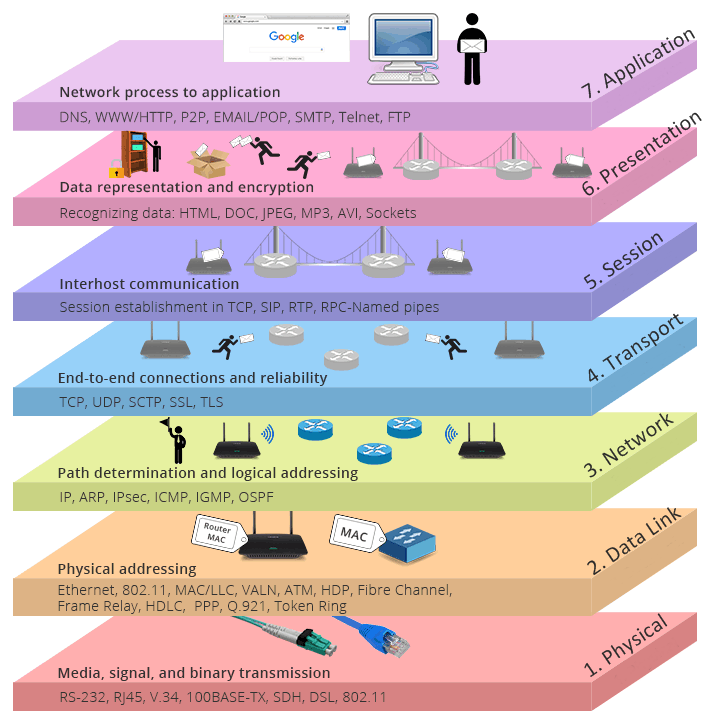
\includegraphics[scale=.45]{Bilder/OSI-Modell1}
	\end{minipage}
	\begin{minipage}{.5\textwidth}
		\textbf{Hauptaufgaben der Schichten:}
        \begin{itemize}
            \item Schicht 7: Anwendungen für Benutzer
            \item Schicht 6: Darstellung der Daten in verständliche Formate (jpg, ASCII)
            \item Schicht 5: Steuerung der Verbindung
            \item Schicht 4: Zuordnung der Datenpakete zu den Ports
            \item Schicht 3: Vermittelt Datenpakete
            \item Schicht 2: Fehlerfreie Übertragung
            \item Schicht 1: Bit-Übertragung 
        \end{itemize}
	\end{minipage}
    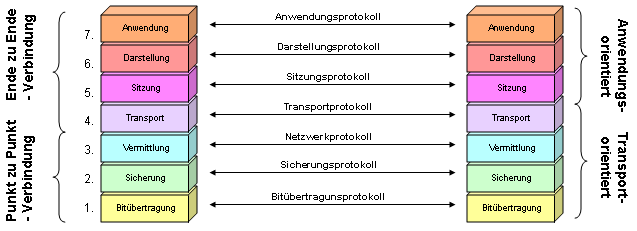
\includegraphics[scale=.75]{Bilder/OSI-Modell2}

\section{Ethernet}
    Mit der Erfindung des Ethernets wollte man individuellen Stationen / Systemen den Zugriff auf ein gemeinsames Medium zur Datenübertragung ermöglichen. Dieses gemeinsame Medium wurde durch ein Koaxial Kabel realisiert.
	\begin{figure}[h]
        \centering
        \begin{tikzpicture}
            \draw[black, very thick] (-1,0) rectangle (1,2);
            \draw[black, very thick] (-4,0) rectangle (-2,2);
            \draw[black, very thick] (2,0) rectangle (4,2);
            \node at (0,1){PC 10};
            \node at (-3,1){PC 01};
            \node at (3,1){PC 11};
            \draw[red, very thick] (-3,0)--(-3,-1);
            \draw[red, very thick] (0,0)--(0,-1);
            \draw[red, very thick] (3,0)--(3,-1);
            \draw[red, very thick] (-5,-1)--(5,-1);
            \draw[black, very thick] (-6,-0.5) rectangle (-5,-1.5);
            \draw[black, very thick] (6,-0.5) rectangle (5,-1.5);
            \node at (-7,-1){Absorber};
            \node at (7,-1){Absorber};
            \node at (0,-1.5){Koax. Kabel};
        \end{tikzpicture}
	\end{figure}\newline
    Soll ein Datenpaket verschickt werden (z.B. ein Zahlenwert), so muss der Sender das Ziel des Paketes kennen, um die Information zum korrekten Empfänger schicken zu können. \newline
    Will \textit{PC 01} die Zahl \textit{5d} an \textit{PC 10} senden, ergibt sich folgender Rahmen:
	\begin{center}
		\begin{tabularx}{14cm}{|X|X|}
			\hline
			0010 \textit{(Kennung des Ziels, 4Bit)}&0101 \textit{(Daten, 4Bit)}\\
			\hline
		\end{tabularx}
	\end{center}
    Damit der Empfänger den Erhalt der Daten quittieren kann, muss jedoch auch die Kennung des Senders im Rahmen enthalten sein:
	\begin{center}
		\begin{tabularx}{17cm}{|X|X|X|}
			\hline
			0010 \textit{(Kennung des Ziels)}&0001 \textit{(Kennung der Quelle)}&0101 \textit{(Daten)}\\
			\hline
		\end{tabularx}
	\end{center}
    Der verschickte Rahmen lautet demnach:
	\begin{center}
		\begin{tabularx}{5cm}{XXX}
			0010&0001&0101\\
		\end{tabularx}
	\end{center}
    Um zu wissen, ob es sich bei den empfangenen Impulsen tatsächlich um eine gesendete Information handelt, wird ein Datenrahmen immer durch eine Präambel angekündigt. Es könnten sonst Missverständnisse durch Signalrauschen oder Störungen auftreten. Die endgültige Struktur eines Datenrahmens:
	\begin{center}
		\begin{tabularx}{17cm}{|l|l|X|X|X|}
			\hline
			Präambel (7Byte)&SFD (1Byte)&Ziel (MAC)&Quelle (MAC)&Nutzdaten\\
			\hline
		\end{tabularx}
	\end{center}

\subsection{MAC Adresse}
    Um Informationen im Ether / Internet zuverlässig und zielgenau verschicken zu können, muss jedes Endgerät im Netz seine eigene individuelle Kennung besitzen!\newline $\longrightarrow$ \emph{MAC Adresse}\newline Die MAC Adresse ist in den ROM der Network Interface Card eines jeden Gerätes eingebrannt. Die MAC ist also keine virtuelle Softwarekennung, sondern eine durchaus physisch mit dem Gerät verbundene Kennnummer.

\subsubsection{Aufbau MAC Adresse}
    \begin{center}
        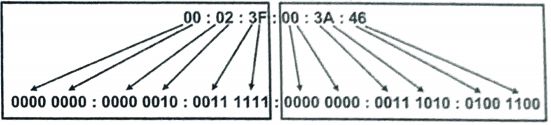
\includegraphics[scale=1]{Bilder/MAC.png}
        \begin{tabularx}{14cm}{XX}
            3 Byte OUI (Herstellerkennung)&3Byte Gerät-Seriennummer
        \end{tabularx}
    \end{center}
    
\section{Netzwerkprotokolle}%Hier gerne noch andere Protokolle :)
    Hat die Netzwerkkarte einen Datenrahmen empfangen, muss ermittelt werden, welches Protokoll zur Weiterverarbeitung verwendet werden soll. Innerhalb des Datenrahmens muss also der Typ und das Ziel der Daten festgelegt sein. Diese Informationen stehen in einem 2Byte großem Typenfeld. Für jedes Protokoll existiert eine eigene Kennung:
    \begin{center}
        \renewcommand{\arraystretch}{1.5}
        \begin{tabularx}{10cm}{|X|X|}
            \hline
            ARP&0x0806\\
            \hline
            IPv4&0x0800\\
            \hline
            IPv6&0x86DD\\
            \hline
        \end{tabularx}
    \end{center}
    Allerdings kommt dem Typenfeld eine weitere Bedeutung:
    \begin{center}
        \renewcommand{\arraystretch}{1.5}
        \begin{tabularx}{14cm}{|X|X|}
            \hline
            Wert kleiner als 0x0600&Länge des Datenrahmens\\
            \hline
            Wert größer als 0x0600&Protokollkennung\\
            \hline
        \end{tabularx}
    \end{center}
    Alle Protokollkennungen müssen also größer als 1536d oder 0x0600h sein!\newline\newline
    \textbf{Achtung:}\newline
    Das ICMP Netzwerkprotokoll ist ein Protokoll der IP-Familie und folgt somit dem IPv4-Protokoll!\newline
    Ebenso gehört das ICMPv6 Netzwerkprotokoll zur IPv6 Familie und folgt somit auch dem IPv6 Protokoll!

\subsection{Datenübertragung}
    Um sicher zu gehen, dass alle Informationen fehlerfrei übertragen wurden, wird dem Datenrahmen ein 4Byte großes Prüffeld (CRC) angehängt. Dieses Prüffeld ergibt sich aus einer Polynomdivision.
    \begin{center}
        \renewcommand{\arraystretch}{1.5}
        \begin{tabularx}{17cm}{|l|l|X|X|X|X|r|}
            \hline
            Präambel&SFD&Ziel-Mac&Quell-MAC&Typ&Nutzdaten&CRC\\
            \hline
        \end{tabularx}
    \end{center}
    \begin{tikzpicture}[remember picture,overlay,thick,black,shorten <=1pt,shorten >=1pt]
        \begin{scope}[c/.style={shift={(-\tabcolsep,\the\dimexpr\fontdimen22\textfont2\relax)}}]
            \draw(3.55,0)--(17,0);
            \draw(3.55,0.5)--(3.55,0);
            \draw(17,0.5)--(17,0);
            \node at (10,-0.5){Min: 64Byte - Max: 1518Byte};
        \end{scope}
    \end{tikzpicture}\newline\newline\newline
    Unterschreitet der Anteil der Nutzdaten 46Byte, wird durch Padding aufgefüllt.

\section{Vollständiges Ethernet-Paket}
    \begin{center}
        \renewcommand{\arraystretch}{1.5}
        \begin{tabularx}{17cm}{|l|l|l|X|X|X|r|}
            \hline
            Präambel 7&SFD 1&Ziel-Mac 6&Quell-MAC 6&Typ 2&Nutzdaten 46-1500&CRC 4\\
            \hline
        \end{tabularx}
    \end{center}
    \begin{center}
        Zahlenwert im Feld = Bytegröße des Feldes.
    \end{center}

\section{CSMA/CD - Verfahren}
    Programmablaufplan des CSMA/CD Verfahrens:
    \begin{center}
        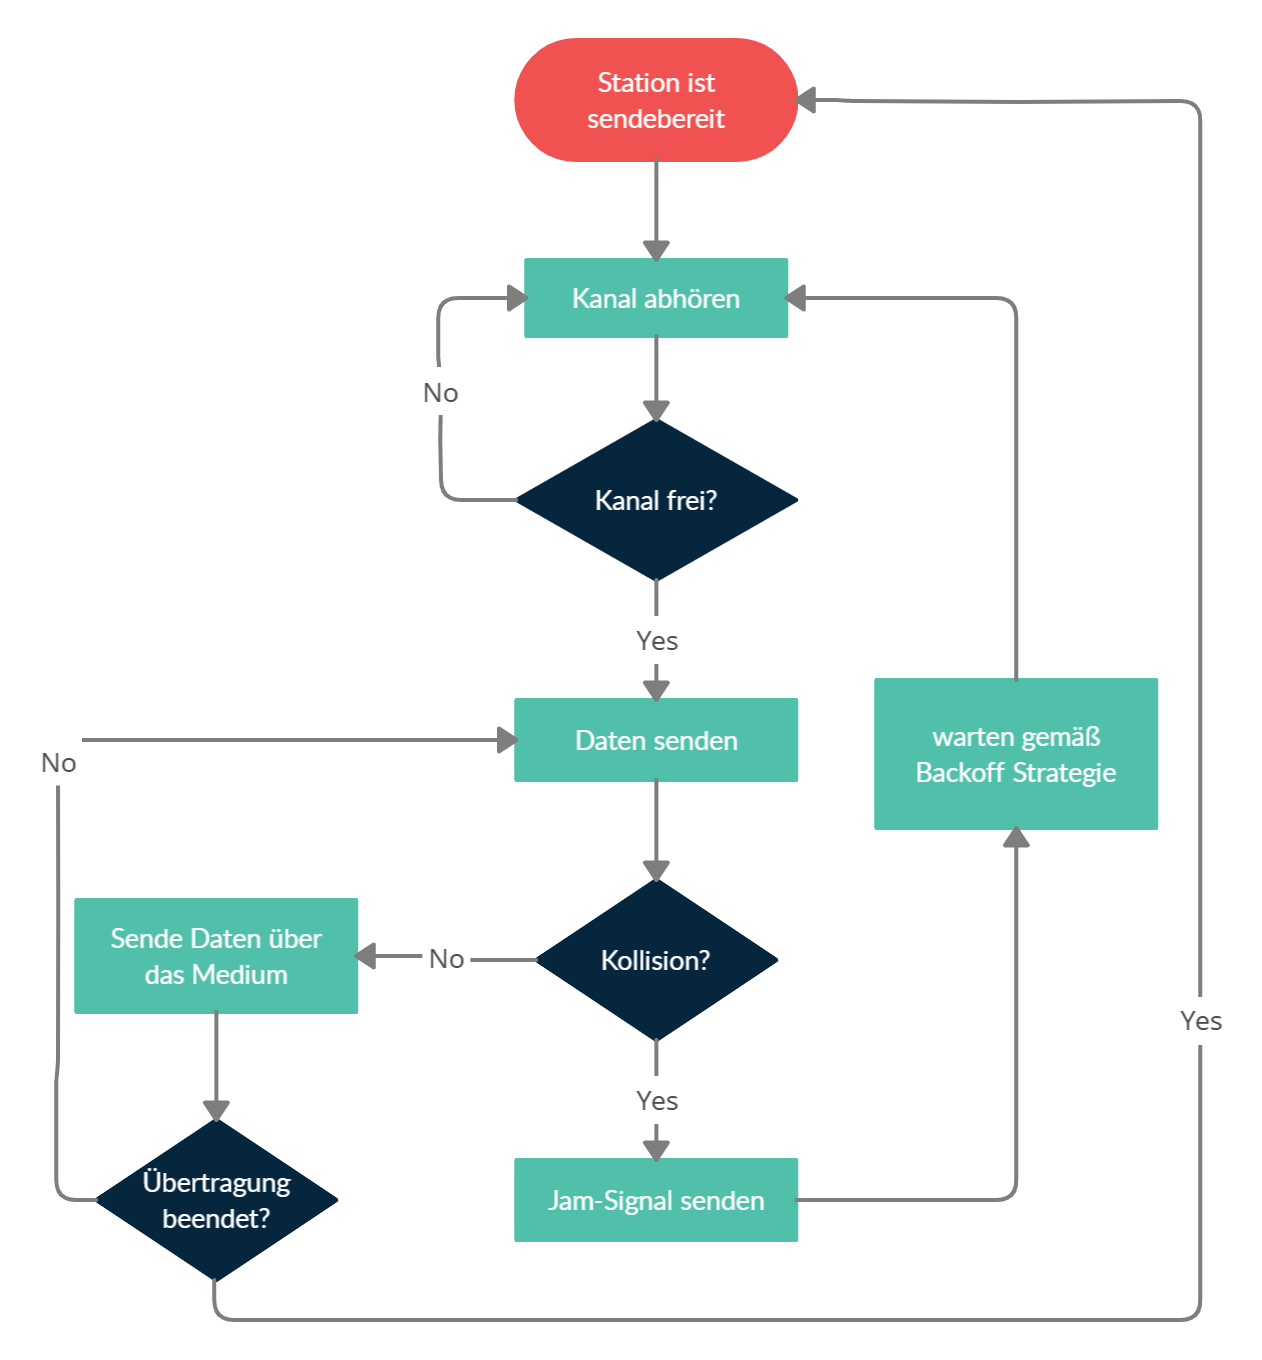
\includegraphics[scale=0.3]{Bilder/CSMACD.png}
    \end{center}

\subsection{Kollision}
    \textbf{Problem:}\newline 
    Da Alle Systeme mit nur einem Übertragungsmedium vernetzt sind, um Materialkosten zu sparen, und Skalierbarkeit zu erhalten, muss der Leiter bidirektional verwendet werden. Dadurch kann es zu Kollisionen von Impulsen kommen.\newline
    $\longrightarrow$ Es kommt zu einer Signalerhöhung / Signalverbreiterung und damit zu einer fehlerhaften Übertragung.\newline\newline
    \textbf{Lösung:}\newline
    CSMA/CD Verfahren - Jam Signal
    \noindent\textbf{Situation:}
    \begin{center}
        \begin{tikzpicture}
            \draw[black, very thick](-7,-1)rectangle(-5,1);
            \draw[black, very thick](7,-1)rectangle(5,1);
            \draw[red, very thick](-5,0)--(5,0);
            \node at (-6,0){PC};
            \node at (6,0){PC};
            \filldraw[fill=green!50,draw=black,very thick](-4.5,0)rectangle(-3.5,1);
            \filldraw[fill=green!50,draw=black,very thick](-2,0)rectangle(0,1);
            \filldraw[fill=blue!50,draw=black,very thick](3,0)rectangle(3.5,1);
            \filldraw[fill=blue!50,draw=black,very thick](1,0)rectangle(2,1);
            \draw[->,black, very thick](-4.5,-0.5)--(-2,-0.5);
            \draw[->,black, very thick](4.5,-0.5)--(2,-0.5);

            \draw[black, very thick](-7,-2)rectangle(-5,-4);
            \draw[black, very thick](7,-2)rectangle(5,-4);
            \draw[red, very thick](-5,-3)--(5,-3);
            \node at (-6,-3){PC};
            \node at (6,-3){PC};
            \filldraw[fill=green!50,draw=black,very thick](-2.5,-3)rectangle(-1.5,-2);
            \filldraw[fill=green!50,draw=black,very thick](0,-3)rectangle(2,-2);
            \filldraw[fill=blue!50,draw=black,very thick](1,-2)rectangle(1.5,-1);
            \filldraw[fill=blue!50,draw=black,very thick](-1,-3)rectangle(0,-2);
            \draw[red, very thick](0.8,-0.8)rectangle(1.7,-3.2);
            \draw[red, very thick](-1.2,-3.2)rectangle(0.2,-1.8);
            \node at (2.2,-3.7){Signalerhöhung};
            \node at (-2,-3.7){Signalverbreiterung};
        \end{tikzpicture}
    \end{center}
    Das sendende System vergleicht ständig das gesendete Signal mit dem Signal auf der Leitung. Kommt es zu Abweichungen bricht das System die Übertragung ab und sendet ein Jam-Signal welches andere Systeme im Netz über die Kollision informiert. Alle Systeme unterbrechen die Übertragung.\newline
    Ab wann dürfen die einzelnen Systeme wieder anfangen Daten zu senden?\newline\newline
    Jedes Signal auf der Leitung braucht eine bestimmte Zeit, um zwischen den beiden entferntesten Systemen im Netz einmal hin, und wieder zurück zu laufen. Diese Zeit wird mit RTT bezeichnet. Ist die RTT abgelaufen, befinden sich keine Signale mehr im Netz, es kann neu gesendet werden. \newline\newline
    Nach dem Ethernet-Standard 802.3 ist die RTT auf 51,2 Mikrosekunden festgelegt.\newline\newline
    Kommt es nach dem Warten der RTT dennoch zu einer weiteren Kollision, variieren die Systeme ihre Wartezeit indem sie ein vielfaches der RTT warten. Als Vielfaches können die Faktoren 0,1,2 und 3 gewählt werden.\newline
    $\longrightarrow$ Es wird unterschiedlich lang gewartet. \newline\newline
    Kommt es erneut zu einer Kollision, wird der Bereich der Vorfaktoren von 0 bis 7 erweitert.
    \begin{center}
        Wartezeit= k $\cdot$ RTD
    \end{center}
    \begin{center}
        k = 0 bis $2^{i}$-1 \hspace{2cm} i = Anzahl Versuche
    \end{center}
    Nach 10 Versuchen wird i nicht mehr erhöht, nach 16 erfolglosen Versuchen wird der Sendeversuch abgebrochen.

\section{ARP-Protokoll}
    Programmablaufplan des ARP Verfahrens:
    \begin{center}
        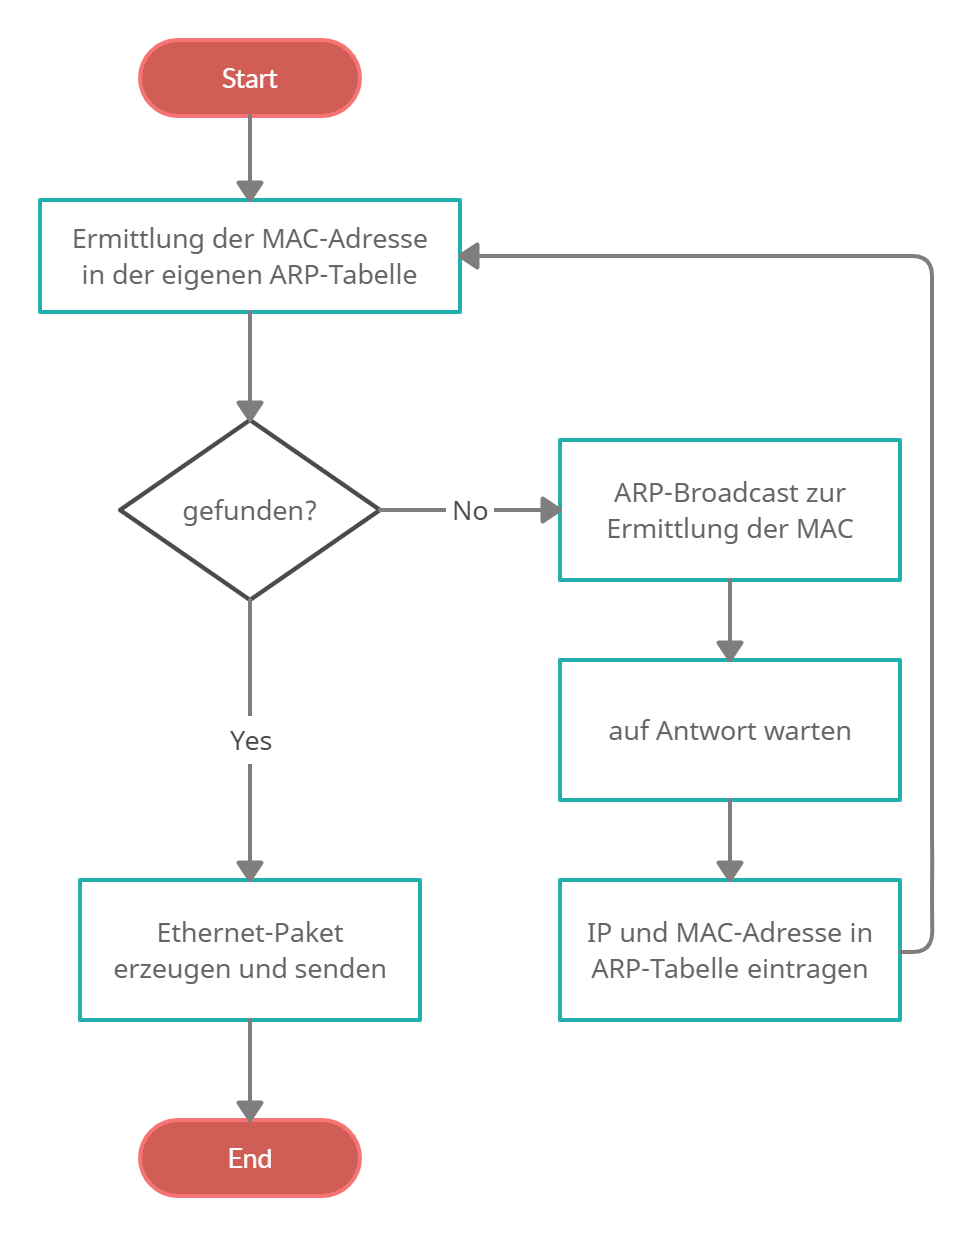
\includegraphics[scale=0.3]{Bilder/ARP-Protokoll PAP.png}
    \end{center}

\section{Subnetting}
    Subnetting ermöglicht es Netzwerkadministratoren beispielsweise, das eigene Firmennetzwerk in Subnetze aufzuteilen, ohne dies im Internet bekannt zu machen. Das heißt, der Router, der schließlich das Netzwerk mit dem Internet verbindet, wird weiterhin als einfache Adresse angegeben.\vspace{.2cm}\\
    Alle Subnetze eines Netzes funktionieren unabhängig voneinander und die Datenvermittlung läuft schneller. Warum ist das so? Subnetting macht das Netzwerk überschaubarer. Ein Broadcast, bei dem ein Teilnehmer Daten an das gesamte Netz sendet, verläuft ohne Ordnung durch Subnetze relativ unkontrolliert.\vspace{.2cm}\\
    Durch Subnets werden Datenpakete durch den Router viel gezielter an die Empfänger geleitet. Befinden sich Sender und Empfänger im gleichen Subnetz, können die Informationen direkt zugestellt und müssen nicht umgeleitet werden.

\subsection{Die IP Adresse}
    Bei dem Netzwerkprotokoll IPv4 (heute aktuell: IPv6) besteht eine IP-Adresse aus 32 Bit. Diese sind in vier Abschnitte mit je einem Oktett aufgeteilt.\\
    Beispiel IP Adresse:
    \begin{center}
        \renewcommand{\arraystretch}{1.5}
        \begin{tabularx}{10cm}{lc}
            dezimal&192.168.0.1 \\
            binär&11000000.10101000.0000000.00000001 \\
        \end{tabularx}
    \end{center}
    Zu beachten ist dabei, dass jedes Oktett als eigenständig bei der Berechnung der Wertigkeit angesehen wird.\\ Der höchste darstellbare Wert eines Oktettes beläuft sich demnach auf 255.
    \begin{center}
        \renewcommand{\arraystretch}{1.5}
        \begin{tabularx}{6cm}{cccccccc}
            $2^7$&$2^6$&$2^5$&$2^4$&$2^3$&$2^2$&$2^1$&$2^0$ \\
            128&46&32&16&8&4&2&1 \\
        \end{tabularx}
    \end{center}

\subsection{Netzwerkklassen}
    Eine IP Adresse ist immer einem bestimmten System, welches sich in einem bestimmten Netz befindet zuzuordnen. Demnach besitzt eine IP Adresse einen Netzwerk und einen Hostbereich. Die IP Adresse muss dazu nicht in der Mitte geteilt sein (2 Oktette Netzwerk, 2 Oktette Hostbereich), sondern kann dazu beliebig zwischen jedem Bit geteilt werden. Netzen, mit 1 Oktett, 2 Oktetten und 3 Oktetten Netzwerkbereich wurden besondere Bezeichnungen zugewiesen:
    \begin{center}
        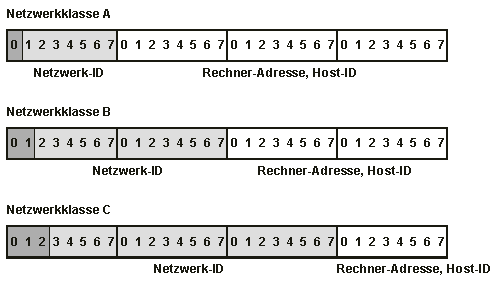
\includegraphics[scale=0.7]{Bilder/Netzwerkklassen.png}
    \end{center}

\subsection{Subnetzmaske}
    Um ein bestehendes Computernetz zur besseren Übersicht und Verwaltung in mehrere kleine Netze aufteilen zu können, bedarf es einer Subnetzmaske. Diese gibt den Netzwerkbereich einer IP Adresse an. Mit Hilfe der Subnetzmaske kann außerdem überprüft werden, ob sich zwei Geräte im gleichen Subnetz befinden oder nicht. Verknüpft man IP Adresse und Subnetzmaske durch eine AND Verknüpfung, erhält man die Netzwerkkennung des Subnetzes, indem sich die IP Adresse befindet. Stimmen die Netzwerkkennungen zweier Systeme überein, befinden sie sich im selben Subnetz.

\subsection{CIDAR}
    Die CIDAR ist eine vereinfachte Schreibweise für die Subnetzmaske. Da eine Subnetzmaske dadurch definiert wird, dass sie in binär Schreibweise eine fortlaufende Kette von gesetzten Bits haben muss, die nicht durch ein nicht gesetztes Bit unterbrochen werden darf, kann man die Schreibweise dahingehend vereinfachen, dass einfach die gesetzten Bits gezählt werden:
    \begin{center}
        \renewcommand{\arraystretch}{1.5}
        \begin{tabularx}{\columnwidth}{XXXXXXXXXXXXXXXXXXXXXXXXXXXXXXXX}
            1&2&3&4&5&6&7&8&9&10&11&12&13&14&15&16&\cellcolor{red!50!white}17&18&19&20&21&22&23&24&25&26&27&28&29&30&31&32 \\
            \hline
            1&1&1&1&1&1&1&1&1&1&1&1&1&1&1&1&1\cellcolor{red!50!white}&0&0&0&0&0&0&0&0&0&0&0&0&0&0&0 \\
        \end{tabularx}\\
        In diesem Falle wäre die CIDAR /17
    \end{center}

\subsection{VLSM}
    VLSM ist ein erweitertes Subnetting. Hierzu wird die Subnetmaske in eine variable Länge gebracht um das Subnetz in mehrere verschieden große Teile zu unterteilen und sie hierarchisch nach ihrer Größe sortiert. Somit ist es möglich, Subnetze mit einer jeweils verschiedenen Anzahl an Hosts zu erschaffen, ohne dass dafür eine große Menge an IP-Adressen verschwendet werden muss.\newline
    \hspace{2cm}
    \textbf{Beispiel:}\newline
    \textcolor{red}{Aufgabenstellung:}\newline
    Es wird ein neues Gebäude gebaut. Dafür steht der IP-Bereich 11.137.4.0/23 zur Verfügung. Die ersten 2 von den 6 Etagen sollen jeweilt 100 IP-Adressen haben und die restlichen 4 jeweils 50 IP-Adressen.
    Gib die IP-Range jeder Etage an!\newline
    \textcolor{red}{Lösung:}\newline
    \textbf{Etage 1:} 11.137.4.1   -  11.137.4.126\newline
    \textbf{Etage 2:} 11.137.4.129 -  11.137.4.254\newline
    \textbf{Etage 3:} 11.137.5.1   -  11.137.5.62 \newline
    \textbf{Etage 4:} 11.137.5.65  -  11.137.5.126\newline
    \textbf{Etage 5:} 11.137.5.129 -  11.137.5.190\newline
    \textbf{Etage 6:} 11.137.5.193 -  11.137.5.254\newline

\subsection{Routing Tabellen}%??? JA oder NEIN?


\subsection{DMZ - Demilitarisierte Zone}
    Eine Demilitarisierte Zone bezeichnet ein Computernetz mit sicherheitstechnisch kontrollierten Zugriffsmöglichkeiten auf die daran angeschlossenen Server. Die in der DMZ aufgestellten Systeme werden durch eine oder mehrere Firewalls gegen andere Netze abgeschirmt.
    \begin{center}
        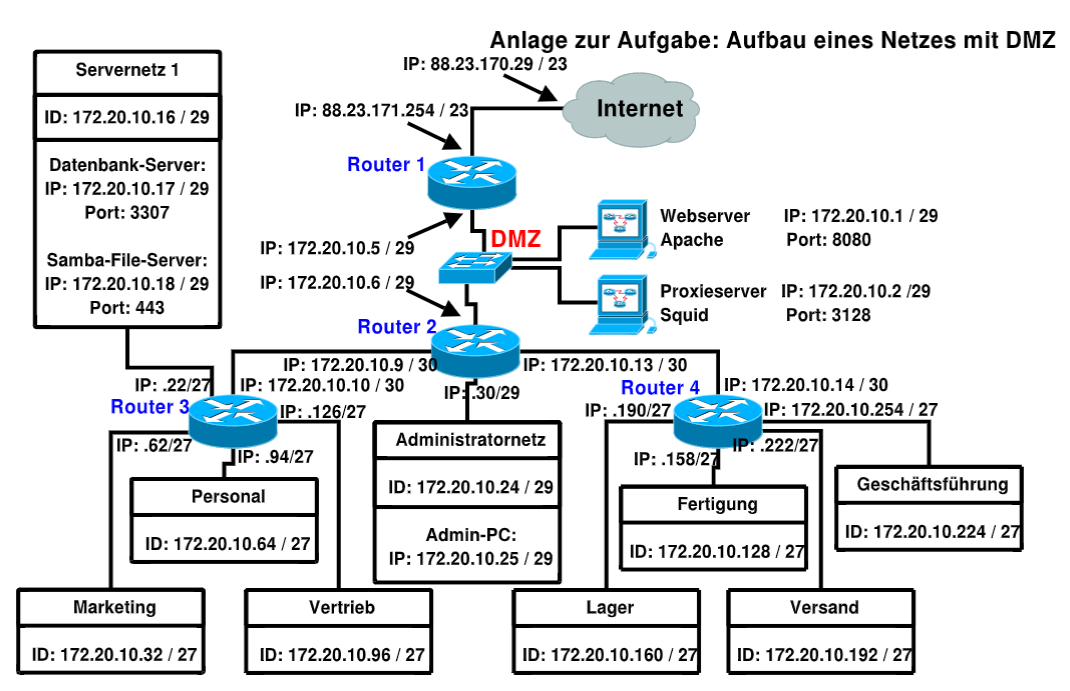
\includegraphics[scale=0.9]{Bilder/DMZ.PNG}
    \end{center}

\subsection{IPv6}
    Vorteile und Nachteile von IPv6 zu IPv4:
    \begin{table}[h]
        \centering
        \begin{tabularx}{17cm}{X|X}
            Vorteile & Nachteile\\
            \hline
            128 Bit = $\text{2}^{\text{128}}$ Adressen & Wenn jedes Gerät eine feste, statische Adresse bekommt, kommt es evtl. zu Sicherheitsrisiken \\
            Kunden bekommen ein /64 Netz &  \\
            \vspace{0.1cm}
            NAT wird nichtmehr gebraucht &  \\
            \vspace{0.1cm}
            Broadcast-Adressen werden nichtmehr gebraucht &  \\
            \vspace{0.1cm}
            ARP wird nichtmehr gebraucht &  \\
            \vspace{0.1cm}
            bis zu 4GiB Datenversandt &  \\
            \vspace{0.1cm}
            verbessertes Multicast &  \\
            \vspace{0.1cm}
        \end{tabularx}
    \end{table}

\section{Schaltnetze}
    Schaltnetze sind Zusammensetzungen von logischen Gattern ohne Speicherverhalten. Sie bestehen aus einem oder mehreren einfachen Bauteilen.
    
\subsection{Einfache Bauteile}
    \subsubsection{NOT}
        Das Not(Negation)-Bauteil negiert das Signal. Somit wird eine Eins zur Null und Nullen werden zu Einsen.
            \begin{center}
                \begin{tikzpicture}
                    \draw[black,very thick] (-5,-1) rectangle (-3,1);
                    \draw[black,very thick] (-6, 0) -- (-5,0);
                    \draw[black,very thick] (-2.8,0) circle (0.2);
                    \draw[black,very thick] (-2.6, 0) -- (-1.6,0);
                    \node at (-4,0){\textbf{1}};
                    \node at (-6.5,0){\textbf{A}};
                    \node at (-1.1,0){\textbf{Z}};

                    \draw[black] (1,0.5) -- (5,0.5);
                    \draw[black] (1,-0.5) -- (5,-0.5);
                    \draw[black] (3,1.5) -- (3,-1.5);
                    \node at (2,1){\textbf{A}};
                    \node at (4,1){\textbf{Z}};
                    \node at (2,0){1};
                    \node at (4,0){0};
                    \node at (2,-1){0};
                    \node at (4,-1){1};
                \end{tikzpicture}
            \end{center}

    \subsubsection{AND}
        Das AND-Bauteil vereint zwei Eingänge zu einem Ausgang. Das Ausgangssignal wird nur Eins, wenn beide Eingangssignale auf Eins standen.
            \begin{center}
                \begin{tikzpicture}
                    \draw[black,very thick] (-5,-1) rectangle (-3,1);
                    \draw[black,very thick] (-6, 0.5) -- (-5,0.5);
                    \draw[black,very thick] (-6, -0.5) -- (-5,-0.5);
                    \draw[black,very thick] (-3, 0) -- (-2,0);
                    \node at (-4,0){\textbf{\&}};
                    \node at (-6.5,0.5){\textbf{A}};
                    \node at (-6.5,-0.5){\textbf{B}};
                    \node at (-1.5,0){\textbf{Z}};

                    \draw[black] (1.5,1.5) -- (4.5,1.5);
                    \draw[black] (1.5,0.5) -- (4.5,0.5);
                    \draw[black] (1.5,-0.5) -- (4.5,-0.5);
                    \draw[black] (1.5,-1.5) -- (4.5,-1.5);
                    \draw[black] (3.5,2.5) -- (3.5,-2.5);
                    \node at (2,2){\textbf{A}};
                    \node at (3,2){\textbf{B}};
                    \node at (4,2){\textbf{Z}};
                    \node at (2,1){0};
                    \node at (3,1){0};
                    \node at (4,1){0};
                    \node at (2,0){0};
                    \node at (3,0){1};
                    \node at (4,0){0};
                    \node at (2,-1){1};
                    \node at (3,-1){0};
                    \node at (4,-1){0};
                    \node at (2,-2){1};
                    \node at (3,-2){1};
                    \node at (4,-2){1};
                \end{tikzpicture}
            \end{center}

    \subsubsection{OR}
        Das OR-Bauteil vereint zwei Eingänge zu einem Ausgang. Das Ausgangssignal wird dann Eins, wenn mindestens einer der Beide Eingangssignale auf Eins steht.
            \begin{center}
                \begin{tikzpicture}
                    \draw[black,very thick] (-5,-1) rectangle (-3,1);
                    \draw[black,very thick] (-6, 0.5) -- (-5,0.5);
                    \draw[black,very thick] (-6, -0.5) -- (-5,-0.5);
                    \draw[black,very thick] (-3, 0) -- (-2,0);
                    \node at (-4,0){\textbf{$\geq 1$}};
                    \node at (-6.5,0.5){\textbf{A}};
                    \node at (-6.5,-0.5){\textbf{B}};
                    \node at (-1.5,0){\textbf{Z}};

                    \draw[black] (1.5,1.5) -- (4.5,1.5);
                    \draw[black] (1.5,0.5) -- (4.5,0.5);
                    \draw[black] (1.5,-0.5) -- (4.5,-0.5);
                    \draw[black] (1.5,-1.5) -- (4.5,-1.5);
                    \draw[black] (3.5,2.5) -- (3.5,-2.5);
                    \node at (2,2){\textbf{A}};
                    \node at (3,2){\textbf{B}};
                    \node at (4,2){\textbf{Z}};
                    \node at (2,1){0};
                    \node at (3,1){0};
                    \node at (4,1){0};
                    \node at (2,0){0};
                    \node at (3,0){1};
                    \node at (4,0){1};
                    \node at (2,-1){1};
                    \node at (3,-1){0};
                    \node at (4,-1){1};
                    \node at (2,-2){1};
                    \node at (3,-2){1};
                    \node at (4,-2){1};
                \end{tikzpicture}
            \end{center}

    \subsubsection{NAND}
        Das NAND-Bauteil vereint zwei Eingänge zu einem Ausgang. Das Ausgangssignal wird dann Eins, wenn mindestens einer der beiden Eingangssignale auf Null steht.
            \begin{center}
                \begin{tikzpicture}
                    \draw[black,very thick] (-5,-1) rectangle (-3,1);
                    \draw[black,very thick] (-6, 0.5) -- (-5,0.5);
                    \draw[black,very thick] (-6, -0.5) -- (-5,-0.5);
                    \draw[black,very thick] (-2.8, 0) circle (0.2);
                    \draw[black,very thick] (-2.6, 0) -- (-2,0);
                    \node at (-4,0){\textbf{\&}};
                    \node at (-6.5,0.5){\textbf{A}};
                    \node at (-6.5,-0.5){\textbf{B}};
                    \node at (-1.5,0){\textbf{Z}};

                    \draw[black] (1.5,1.5) -- (4.5,1.5);
                    \draw[black] (1.5,0.5) -- (4.5,0.5);
                    \draw[black] (1.5,-0.5) -- (4.5,-0.5);
                    \draw[black] (1.5,-1.5) -- (4.5,-1.5);
                    \draw[black] (3.5,2.5) -- (3.5,-2.5);
                    \node at (2,2){\textbf{A}};
                    \node at (3,2){\textbf{B}};
                    \node at (4,2){\textbf{Z}};
                    \node at (2,1){0};
                    \node at (3,1){0};
                    \node at (4,1){1};
                    \node at (2,0){0};
                    \node at (3,0){1};
                    \node at (4,0){1};
                    \node at (2,-1){1};
                    \node at (3,-1){0};
                    \node at (4,-1){1};
                    \node at (2,-2){1};
                    \node at (3,-2){1};
                    \node at (4,-2){0};
                \end{tikzpicture}
            \end{center}

    \subsubsection{NOR}
        Das NOR-Bauteil vereint zwei Eingänge zu einem Ausgang. Das Ausgangssignal wird dann Eins, wenn beide Eingangssignale auf Null steht.
            \begin{center}
                \begin{tikzpicture}
                    \draw[black,very thick] (-5,-1) rectangle (-3,1);
                    \draw[black,very thick] (-6, 0.5) -- (-5,0.5);
                    \draw[black,very thick] (-6, -0.5) -- (-5,-0.5);
                    \draw[black,very thick] (-2.8, 0) circle (0.2);
                    \draw[black,very thick] (-2.6, 0) -- (-2,0);
                    \node at (-4,0){\textbf{$\geq 1$}};
                    \node at (-6.5,0.5){\textbf{A}};
                    \node at (-6.5,-0.5){\textbf{B}};
                    \node at (-1.5,0){\textbf{Z}};

                    \draw[black] (1.5,1.5) -- (4.5,1.5);
                    \draw[black] (1.5,0.5) -- (4.5,0.5);
                    \draw[black] (1.5,-0.5) -- (4.5,-0.5);
                    \draw[black] (1.5,-1.5) -- (4.5,-1.5);
                    \draw[black] (3.5,2.5) -- (3.5,-2.5);
                    \node at (2,2){\textbf{A}};
                    \node at (3,2){\textbf{B}};
                    \node at (4,2){\textbf{Z}};
                    \node at (2,1){0};
                    \node at (3,1){0};
                    \node at (4,1){1};
                    \node at (2,0){0};
                    \node at (3,0){1};
                    \node at (4,0){0};
                    \node at (2,-1){1};
                    \node at (3,-1){0};
                    \node at (4,-1){0};
                    \node at (2,-2){1};
                    \node at (3,-2){1};
                    \node at (4,-2){0};
                \end{tikzpicture}
            \end{center}
    
    \subsubsection{XOR}
        Das XOR-Bauteil vereint zwei Eingänge zu einem Ausgang. Das Ausgangssignal wird dann Eins, wenn die Eingangssignale ungleich sind.
            \begin{center}
                \begin{tikzpicture}
                    \draw[black,very thick] (-5,-1) rectangle (-3,1);
                    \draw[black,very thick] (-6, 0.5) -- (-5,0.5);
                    \draw[black,very thick] (-6, -0.5) -- (-5,-0.5);
                    \draw[black,very thick] (-2.8, 0) circle (0.2);
                    \draw[black,very thick] (-2.6, 0) -- (-2,0);
                    \node at (-4,0){\textbf{=1}};
                    \node at (-6.5,0.5){\textbf{A}};
                    \node at (-6.5,-0.5){\textbf{B}};
                    \node at (-1.5,0){\textbf{Z}};

                    \draw[black] (1.5,1.5) -- (4.5,1.5);
                    \draw[black] (1.5,0.5) -- (4.5,0.5);
                    \draw[black] (1.5,-0.5) -- (4.5,-0.5);
                    \draw[black] (1.5,-1.5) -- (4.5,-1.5);
                    \draw[black] (3.5,2.5) -- (3.5,-2.5);
                    \node at (2,2){\textbf{A}};
                    \node at (3,2){\textbf{B}};
                    \node at (4,2){\textbf{Z}};
                    \node at (2,1){0};
                    \node at (3,1){0};
                    \node at (4,1){0};
                    \node at (2,0){0};
                    \node at (3,0){1};
                    \node at (4,0){1};
                    \node at (2,-1){1};
                    \node at (3,-1){0};
                    \node at (4,-1){1};
                    \node at (2,-2){1};
                    \node at (3,-2){1};
                    \node at (4,-2){0};
                \end{tikzpicture}
            \end{center}

    \subsubsection{XNOR}
        Das XNOR-Bauteil vereint zwei Eingänge zu einem Ausgang. Das Ausgangssignal wird dann Eins, wenn die beiden Eingangssignale gleich stehen.
        \begin{center}
            \begin{tikzpicture}
                \draw[black,very thick] (-5,-1) rectangle (-3,1);
                \draw[black,very thick] (-6, 0.5) -- (-5,0.5);
                \draw[black,very thick] (-6, -0.5) -- (-5,-0.5);
                \draw[black,very thick] (-2.8, 0) circle (0.2);
                \draw[black,very thick] (-2.6, 0) -- (-2,0);
                \node at (-4,0){\textbf{=}};
                \node at (-6.5,0.5){\textbf{A}};
                \node at (-6.5,-0.5){\textbf{B}};
                \node at (-1.5,0){\textbf{Z}};

                \draw[black] (1.5,1.5) -- (4.5,1.5);
                \draw[black] (1.5,0.5) -- (4.5,0.5);
                \draw[black] (1.5,-0.5) -- (4.5,-0.5);
                \draw[black] (1.5,-1.5) -- (4.5,-1.5);
                \draw[black] (3.5,2.5) -- (3.5,-2.5);
                \node at (2,2){\textbf{A}};
                \node at (3,2){\textbf{B}};
                \node at (4,2){\textbf{Z}};
                \node at (2,1){0};
                \node at (3,1){0};
                \node at (4,1){1};
                \node at (2,0){0};
                \node at (3,0){1};
                \node at (4,0){0};
                \node at (2,-1){1};
                \node at (3,-1){0};
                \node at (4,-1){0};
                \node at (2,-2){1};
                \node at (3,-2){1};
                \node at (4,-2){1};
            \end{tikzpicture}
        \end{center}

\subsection{Wahrheitstabelle}
    Die Wahrheitstabelle stellt alle möglichen Zustände einer Schaltung dar. Sie sieht für folgende Schaltung folgendermaßen aus:
    \begin{center}
        \begin{tikzpicture}
            \draw[black,very thick] (-8,-1) rectangle (-6,1);
            \draw[black,very thick] (-9, 0.5) -- (-8,0.5);
            \draw[black,very thick] (-9, -0.5) -- (-8,-0.5);
            \draw[black,very thick] (-6, 0) -- (-4,0);
            \node at (-7,0){\textbf{\&}};
            \node at (-9.5,0.5){\textbf{A}};
            \node at (-9.5,-0.5){\textbf{B}};
            \node at (-5.5,0.5){\textbf{X}};

            \draw[black,very thick] (-7,-4) rectangle (-5,-2);
            \draw[black,very thick] (-8.5, -2.5) -- (-8.5,-0.5);
            \filldraw[black, very thick](-8.5,-0.5) circle(0.1);
            \draw[black,very thick] (-8.5, -2.5) -- (-7,-2.5);
            \draw[black,very thick] (-9, -3.5) -- (-7,-3.5);
            \draw[black,very thick] (-5, -3) -- (-4,-3);
            \node at (-6,-3){\textbf{$\geq 1$}};
            \node at (-9.5,-3.5){\textbf{C}};
            \node at (-4.5,-2.5){\textbf{Y}};

            \draw[black,very thick] (-3.5,-3) rectangle (-1.5,-1);
            \draw[black,very thick] (-1.5,-2) -- (-0.5,-2);
            \draw[black,very thick] (-4,-3) -- (-4,-2.5);
            \draw[black,very thick] (-4,-2.5) -- (-3.5,-2.5);
            \draw[black,very thick] (-4,0) -- (-4,-1.5);
            \draw[black,very thick] (-4,-1.5) -- (-3.5,-1.5);
            \node at (-2.5,-2){\textbf{\&}};
            \node at (0,-2){\textbf{Z}};

            \draw[black] (1.5,0.5) -- (5.5,0.5);
            \draw[black] (4.5,1.5) -- (4.5,-4);
            \node at (2,1){\textbf{C}};
            \node at (3,1){\textbf{B}};
            \node at (4,1){\textbf{A}};
            \node at (5,1){\textbf{Z}};
            \node at (2,0){0};
            \node at (3,0){0};
            \node at (4,0){0};
            \node at (5,0){0};
            \node at (2,-0.5){0};
            \node at (3,-0.5){0};
            \node at (4,-0.5){1};
            \node at (5,-0.5){0};
            \node at (2,-1){0};
            \node at (3,-1){1};
            \node at (4,-1){0};
            \node at (5,-1){0};
            \node at (2,-1.5){0};
            \node at (3,-1.5){1};
            \node at (4,-1.5){1};
            \node at (5,-1.5){1};
            \node at (2,-2){1};
            \node at (3,-2){0};
            \node at (4,-2){0};
            \node at (5,-2){0};
            \node at (2,-2.5){1};
            \node at (3,-2.5){0};
            \node at (4,-2.5){1};
            \node at (5,-2.5){0};
            \node at (2,-3){1};
            \node at (3,-3){1};
            \node at (4,-3){0};
            \node at (5,-3){0};
            \node at (2,-3.5){1};
            \node at (3,-3.5){1};
            \node at (4,-3.5){1};
            \node at (5,-3.5){1};
        \end{tikzpicture}
    \end{center}

\subsection{KV-Diagramm}
    Die Nummern im KV-Diagramm ergeben den dezimalen Wert, des entstehenden Binärcodes(siehe Wahrheitstabelle). Die Disjunktiven Normalformen der Schaltfunktionen lassen sich mit dem KV-Diagramm erheblich leichter kürzen! Man sucht aneinander liegende Einsen und bestimmt deren Gemeinsamkeiten. Jede „1“ darf nur in einem Größeren Bereich verwendet werden, somit müssen möglichst viele Felder zu Einem gruppiert werden.
    \begin{center}
        \begin{tikzpicture}
            \draw[black,very thick](1,-5) rectangle (5,-1);
            \draw[black,very thick](1,-2) -- (6,-2);
            \draw[black,very thick](0,-3) -- (5,-3);
            \draw[black,very thick](1,-4) -- (6,-4);
            \draw[black,very thick](2,-1) -- (2,-6);
            \draw[black,very thick](3,0) -- (3,-5);
            \draw[black,very thick](4,-1) -- (4,-6);
            \node at (2,-0.5){A};
            \node at (4,-0.5){$\mathbf{\bar{A}}$};
            \node at (0.5,-2){B};
            \node at (0.5,-4){$\mathbf{\bar{B}}$};
            \node at (3,-5.5){C};
            \node at (1.5,-5.5){$\mathbf{\bar{C}}$};
            \node at (4.5,-5.5){$\mathbf{\bar{C}}$};
            \node at (5.5,-3){D};
            \node at (5.5,-1.5){$\mathbf{\bar{D}}$};
            \node at (5.5,-4.5){$\mathbf{\bar{D}}$};

            \node[red] at (1.5,-1.5){3};
            \node[red] at (2.5,-1.5){7};
            \node[red] at (3.5,-1.5){6};
            \node[red] at (4.5,-1.5){2};
            \node[red] at (1.5,-2.5){11};
            \node[red] at (2.5,-2.5){15};
            \node[red] at (3.5,-2.5){14};
            \node[red] at (4.5,-2.5){10};
            \node[red] at (1.5,-3.5){9};
            \node[red] at (2.5,-3.5){13};
            \node[red] at (3.5,-3.5){12};
            \node[red] at (4.5,-3.5){8};
            \node[red] at (1.5,-4.5){1};
            \node[red] at (2.5,-4.5){5};
            \node[red] at (3.5,-4.5){4};
            \node[red] at (4.5,-4.5){0};
        \end{tikzpicture}
    \end{center}
\textbf{Beispiel:}\\
Für folgende Wahrheitstabelle sieht das KV-Diagramm folgendermaßen aus:
    \begin{center}
        \begin{tikzpicture}
            \draw[black] (-7.5,0.5) -- (-2.5,0.5);
            \draw[black] (-3.5,1.5) -- (-3.5,-8);
            \node at (-7,1){\textbf{D}};
            \node at (-6,1){\textbf{C}};
            \node at (-5,1){\textbf{B}};
            \node at (-4,1){\textbf{A}};
            \node at (-3,1){\textbf{Z}};
            \node at (-7,0){0};
            \node at (-6,0){0};
            \node at (-5,0){0};
            \node at (-4,0){0};
            \node at (-3,0){0};
            \node at (-7,-0.5){0};
            \node at (-6,-0.5){0};
            \node at (-5,-0.5){0};
            \node at (-4,-0.5){1};
            \node at (-3,-0.5){0};
            \node at (-7,-1){0};
            \node at (-6,-1){0};
            \node at (-5,-1){1};
            \node at (-4,-1){0};
            \node at (-3,-1){0};
            \node at (-7,-1.5){0};
            \node at (-6,-1.5){0};
            \node at (-5,-1.5){1};
            \node at (-4,-1.5){1};
            \node at (-3,-1.5){1};
            \node at (-7,-2){0};
            \node at (-6,-2){1};
            \node at (-5,-2){0};
            \node at (-4,-2){0};
            \node at (-3,-2){0};
            \node at (-7,-2.5){0};
            \node at (-6,-2.5){1};
            \node at (-5,-2.5){0};
            \node at (-4,-2.5){1};
            \node at (-3,-2.5){0};
            \node at (-7,-3){0};
            \node at (-6,-3){1};
            \node at (-5,-3){1};
            \node at (-4,-3){0};
            \node at (-3,-3){0};
            \node at (-7,-3.5){0};
            \node at (-6,-3.5){1};
            \node at (-5,-3.5){1};
            \node at (-4,-3.5){1};
            \node at (-3,-3.5){1};
            \node at (-7,-4){1};
            \node at (-6,-4){0};
            \node at (-5,-4){0};
            \node at (-4,-4){0};
            \node at (-3,-4){0};
            \node at (-7,-4.5){1};
            \node at (-6,-4.5){0};
            \node at (-5,-4.5){0};
            \node at (-4,-4.5){1};
            \node at (-3,-4.5){0};
            \node at (-7,-5){1};
            \node at (-6,-5){0};
            \node at (-5,-5){1};
            \node at (-4,-5){0};
            \node at (-3,-5){0};
            \node at (-7,-5.5){1};
            \node at (-6,-5.5){0};
            \node at (-5,-5.5){1};
            \node at (-4,-5.5){1};
            \node at (-3,-5.5){1};
            \node at (-7,-6){1};
            \node at (-6,-6){1};
            \node at (-5,-6){0};
            \node at (-4,-6){0};
            \node at (-3,-6){0};
            \node at (-7,-6.5){1};
            \node at (-6,-6.5){1};
            \node at (-5,-6.5){0};
            \node at (-4,-6.5){1};
            \node at (-3,-6.5){0};
            \node at (-7,-7){1};
            \node at (-6,-7){1};
            \node at (-5,-7){1};
            \node at (-4,-7){0};
            \node at (-3,-7){0};
            \node at (-7,-7.5){1};
            \node at (-6,-7.5){1};
            \node at (-5,-7.5){1};
            \node at (-4,-7.5){1};
            \node at (-3,-7.5){1};

            \node[red] at (-8,0){0};
            \node[red] at (-8,-0.5){1};
            \node[red] at (-8,-1){2};
            \node[red] at (-8,-1.5){3};
            \node[red] at (-8,-2){4};
            \node[red] at (-8,-2.5){5};
            \node[red] at (-8,-3){6};
            \node[red] at (-8,-3.5){7};
            \node[red] at (-8,-4){8};
            \node[red] at (-8,-4.5){9};
            \node[red] at (-8,-5){10};
            \node[red] at (-8,-5.5){11};
            \node[red] at (-8,-6){12};
            \node[red] at (-8,-6.5){13};
            \node[red] at (-8,-7){14};
            \node[red] at (-8,-7.5){15};
            
            \draw[black,very thick](1,-5) rectangle (5,-1);
            \draw[black,very thick](1,-2) -- (6,-2);
            \draw[black,very thick](0,-3) -- (5,-3);
            \draw[black,very thick](1,-4) -- (6,-4);
            \draw[black,very thick](2,-1) -- (2,-6);
            \draw[black,very thick](3,0) -- (3,-5);
            \draw[black,very thick](4,-1) -- (4,-6);
            \node at (2,-0.5){A};
            \node at (4,-0.5){$\mathbf{\bar{A}}$};
            \node at (0.5,-2){B};
            \node at (0.5,-4){$\mathbf{\bar{B}}$};
            \node at (3,-5.5){C};
            \node at (1.5,-5.5){$\mathbf{\bar{C}}$};
            \node at (4.5,-5.5){$\mathbf{\bar{C}}$};
            \node at (5.5,-3){D};
            \node at (5.5,-1.5){$\mathbf{\bar{D}}$};
            \node at (5.5,-4.5){$\mathbf{\bar{D}}$};

            \node at (1.5,-1.5){1};
            \node at (2.5,-1.5){1};
            \node at (3.5,-1.5){0};
            \node at (4.5,-1.5){0};
            \node at (1.5,-2.5){1};
            \node at (2.5,-2.5){1};
            \node at (3.5,-2.5){0};
            \node at (4.5,-2.5){0};
            \node at (1.5,-3.5){0};
            \node at (2.5,-3.5){0};
            \node at (3.5,-3.5){0};
            \node at (4.5,-3.5){0};
            \node at (1.5,-4.5){0};
            \node at (2.5,-4.5){0};
            \node at (3.5,-4.5){0};
            \node at (4.5,-4.5){0};

            \draw[green,very thick](1.2,-1.2) rectangle (2.8,-2.8);
            \node[green,very thick] at (3,-7){$Z=A \wedge B$};
        \end{tikzpicture}
    \end{center}

\subsubsection{Don't-Care-Positions}
    Don't-Care-Positions sind Zustände bei welchen der Zustandswert egal ist. Im KV-Diagramm wird hierfür ein X eingetragen. Don't-Care-Positions können auch mit als Kästen zusammengefasst werden.

\subsection{Disjunktive Normalform}
    Die Disjunktive Normalform ist ein ungekürzter Term für die Bestimmung eines Ausgangssignales. Mit ihr kann das Ausgangssignal bei bekannten Eingangswerten bestimmt werden.

\subsection{Impulsdiagramm}
    Das Impulsdiagramm zeigt die Highs und Lows der Ein- und Ausgänge, also quasi eine bildliche Wahrheitstabelle
    \begin{center}
        \begin{minipage}{.45\textwidth}
            \begin{center}
                \begin{tikzpicture}
                    \draw(0,0)rectangle(7,-4);
                    \node at (0.7,-0.3){\textbf{ODER}};
                    \node at (1,-1.5){$X_1$};
                    \node at (1,-2.5){$X_2$};
                    \draw(1.5,-1.5)--(2.5,-1.5);
                    \draw(1.5,-2.5)--(2.5,-2.5);
                    \draw(2.5,-1)rectangle(4.5,-3);
                    \node at (3.5,-2){$\geqq$1};
                    \draw(4.5,-2)--(5.5,-2);
                    \node at (6,-2){Y};
                \end{tikzpicture}
                \begin{tikzpicture}
                    \draw(0,0)rectangle(7,-2);
                    \node at (0.8,-0.3){\textbf{Formel}};
                    \node at (3.5,-1){$\mathbf{Y = X_1 \lor X_2}$};
                \end{tikzpicture}
            \end{center}
        \end{minipage}	   
        \hspace{.5cm}
        \begin{minipage}{.45\textwidth}
            \begin{center}
                \renewcommand{\arraystretch}{1.7}
                \begin{tabularx}{\columnwidth}{|X|X|X|}
                    \hline
                    \multicolumn{3}{|l|}{Wahrheitstabelle}\\
                    \hline
                    Eingang&Eingang&Ausgang \\
                    $X_1$&$X_2$&Y \\
                    \hline
                    0&0&0 \\
                    \hline
                    0&1&1 \\
                    \hline
                    1&0&1 \\
                    \hline
                    1&1&1 \\
                    \hline
                \end{tabularx}
            \end{center}			
        \end{minipage}\newline
        \textcolor{white}{Abstandhalter}	
        \begin{tikzpicture}
            \draw(0,0)rectangle(15.7,-5.2);
            \node at (1.8,-0.3){\textbf{Impulsdiagramm}};
            \node at (1.75,-1.5){$X_1$};
            \node at (1.75,-3){$X_2$};
            \node at (1.75,-4.5){Y};
            \draw[dotted, very thick](2.5,-2)--(13.5,-2);
            \draw[dotted, very thick](2.5,-3.5)--(13.5,-3.5);
            \draw[dotted, very thick](2.5,-5)--(13.5,-5);
            \draw[dotted, very thick](2.5,-1)--(13.5,-1);
            \draw[dotted, very thick](2.5,-2.5)--(13.5,-2.5);
            \draw[dotted, very thick](2.5,-4)--(13.5,-4);
            \node at (2.3,-2){0};
            \node at (2.3,-1){1};
            \node at (2.3,-3.5){0};
            \node at (2.3,-2.5){1};
            \node at (2.3,-5){0};
            \node at (2.3,-4){1};
            \draw[gray] (3,-1)--(3,-5);
            \draw[gray] (5,-1)--(5,-5);
            \draw[gray] (7,-1)--(7,-5);
            \draw[gray] (9,-1)--(9,-5);
            \draw[gray] (11,-1)--(11,-5);
            \draw[gray] (13,-1)--(13,-5);
            \draw[orange, line width = 1.5pt](2.5,-2)--(3,-2)--(3,-1)--(5,-1)--(5,-2)--(7,-2)--(7,-1)--(9,-1)--(9,-2)--(11,-2)--(11,-1)--(13,-1)--(13,-2)--(13.5,-2);
            \draw[cyan, line width = 1.5pt](2.5,-3.5)--(3,-3.5)--(3,-2.5)--(7,-2.5)--(7,-3.5)--(13,-3.5)--(13,-2.5)--(13.5,-2.5);
            \draw[red, line width = 1.5pt](2.5,-5)--(3,-5)--(3,-4)--(9,-4)--(9,-5)--(11,-5)--(11,-4)--(13.5,-4);
        \end{tikzpicture}
    \end{center}

\subsection{Zustandsfolgetabelle}
    Die Zustandsfolgetabelle gibt die aktuelle und Übergangsfunktion für ein Schaltwerk oder Schaltnetz.
    \begin{center}
        \begin{tikzpicture}
            \draw[black,very thick] (-5,-1) -- (-5,1);
            \draw[black,very thick] (-5,1) -- (-3,1);
            \draw[black,very thick] (-3,-1) -- (-3,1);
            \draw[black,very thick] (-6, 0) -- (-5,0);
            \node at (-4,0.5){\textbf{Counter}};
            \node at (-6.5,0){\textbf{Takt}};
            \draw[black,very thick] (-5, 0.3) -- (-4.7,0);
            \draw[black,very thick] (-5, -0.3) -- (-4.7,0);
            \draw[black,very thick] (-5, -1) -- (-4.5,-1) -- (-4.5,-1.5);
            \draw[black,very thick] (-3, -1) -- (-3.5,-1) -- (-3.5,-1.5);
            \draw[black,very thick] (-5,-1.5) rectangle (-3,-4.5);
            \draw[black,very thick] (-5,-2.5) -- (-3,-2.5);
            \draw[black,very thick] (-5,-3.5) -- (-3,-3.5);
            \draw[black,very thick] (-2,-2) -- (-3,-2);
            \draw[black,very thick] (-2,-3) -- (-3,-3);
            \draw[black,very thick] (-2,-4) -- (-3,-4);
            \node at (-1.5,-2){Q1};
            \node at (-1.5,-3){Q2};
            \node at (-1.5,-4){Q3};

            \draw[black] (0.5,1.5) -- (6.5,1.5);
            \draw[black] (3.5,2.5) -- (3.5,-6.5);
            \node[red] at (2,3){$t_{n}$};
            \node[red] at (5,3){$t_{n+1}$};
            \node at (1,2){\textbf{Q3}};
            \node at (2,2){\textbf{Q2}};
            \node at (3,2){\textbf{Q1}};
            \node at (4,2){\textbf{Q3}};
            \node at (5,2){\textbf{Q2}};
            \node at (6,2){\textbf{Q1}};
            \node at (1,1){0};
            \node at (2,1){0};
            \node at (3,1){0};
            \node at (4,1){0};
            \node at (5,1){0};
            \node at (6,1){1};
            \node at (1,0){0};
            \node at (2,0){0};
            \node at (3,0){1};
            \node at (4,0){0};
            \node at (5,0){1};
            \node at (6,0){0};
            \node at (1,-1){0};
            \node at (2,-1){1};
            \node at (3,-1){0};
            \node at (4,-1){0};
            \node at (5,-1){1};
            \node at (6,-1){1};
            \node at (1,-2){0};
            \node at (2,-2){1};
            \node at (3,-2){1};
            \node at (4,-2){1};
            \node at (5,-2){0};
            \node at (6,-2){0};
            \node at (1,-3){1};
            \node at (2,-3){0};
            \node at (3,-3){0};
            \node at (4,-3){1};
            \node at (5,-3){0};
            \node at (6,-3){1};
            \node at (1,-4){1};
            \node at (2,-4){0};
            \node at (3,-4){1};
            \node at (4,-4){1};
            \node at (5,-4){1};
            \node at (6,-4){0};
            \node at (1,-5){1};
            \node at (2,-5){1};
            \node at (3,-5){0};
            \node at (4,-5){1};
            \node at (5,-5){1};
            \node at (6,-5){1};
            \node at (1,-6){1};
            \node at (2,-6){1};
            \node at (3,-6){1};
            \node at (4,-6){0};
            \node at (5,-6){0};
            \node at (6,-6){0};
        \end{tikzpicture}
    \end{center}

\section{Schaltwerke}

\subsection{Schaltwerke}
    Schaltwerke besitzen Speicherverhalten, d.h. der Ausgabewert hängt nicht nur von der Eingabe, sondern auch vom Zustand des Schaltwerks ab.

\subsection{Taktgeber}
    Der Taktgeber gibt einen Takt. Dieser wechselt zwischen Einsen und Nullen. Meist wird die Geschwindigkeit als Frequenz angegeben. Die Zeit $t$ zwischen den Wechseln, wird berechnet durch: $t=\frac{1}{f}$
    \begin{center}
        \begin{tikzpicture}
            \draw[black,very thick](-1.5,-1) rectangle (0.5,1);
            \draw[black,very thick](0.5,0) -- (1.5,0);
            \draw[black,very thick](-1,-0.3)--(-0.8,-0.3)--(-0.8,-0.1)--(-0.6,-0.1)--(-0.6,-0.3)--(-0.4,-0.3)--(-0.4,-0.1)--(-0.2,-0.1)--(-0.2,-0.3)--(0,-0.3);
            \node at (-0.5,0.5){10Hz};
        \end{tikzpicture}
    \end{center}

\subsection{Flip-Flops}
    Flip Flops sind Speichereinheiten, welche ein Signal zwischenspeichern können.

\subsubsection{RS Flip Flop}
    Das RS Flip Flop kann Signale speichern und behält diese bis sie rückgesetzt werden. Hierfür gibt es 3 Eingänge. Der erste Eingang ist R für Rücksetzen, der zweite ist der Takt und der dritte ist S fürs Setzen. Es ist Taktflanken gesteuert und das Signal tritt bei aufsteigender Flanke ein.
    \begin{center}
        \begin{tikzpicture}
            \draw[black,very thick](-4,-2.5) rectangle (-1,1.5);
            \draw[black,very thick](-5,0.5) -- (-4,0.5);
            \draw[black,very thick](-5,-0.5) -- (-4,-0.5);
            \draw[black,very thick](-5,-1.5) -- (-4,-1.5);
            \draw[black,very thick](-4,-0.2) -- (-3.7,-0.5) -- (-4,-0.8);
            \draw[black,very thick](-1,-0.5) -- (0,-0.5);
            \node at (-3.5,0.5){\textbf{R}};
            \node at (-3.5,-1.5){\textbf{S}};
            \node at (0.5,-0.5){\textbf{Q}};

            \draw[black,very thick](2,1) -- (6,1);
            \draw[black,very thick](4.5,2) -- (4.5,-3);
            \node at (2.5,1.5){\textbf{Takt}};
            \node at (3.5,1.5){\textbf{R}};
            \node at (4,1.5){\textbf{S}};
            \node at (5.5,1.5){\textbf{Q$^{n+1}$}};
            \node at (2.5,0.5){$\uparrow$};
            \node at (3.5,0.5){0};
            \node at (4,0.5){0};
            \node at (5.5,0.5){Q$^n$};
            \node at (2.5,-0.5){$\uparrow$};
            \node at (3.5,-0.5){1};
            \node at (4,-0.5){0};
            \node at (5.5,-0.5){0};
            \node at (2.5,-1.5){$\uparrow$};
            \node at (3.5,-1.5){0};
            \node at (4,-1.5){1};
            \node at (5.5,-1.5){1};
            \node at (2.5,-2.5){$\uparrow$};
            \node at (3.5,-2.5){1};
            \node at (4,-2.5){1};
            \node at (5.5,-2.5){undefined};
        \end{tikzpicture}
    \end{center}

\subsubsection{T Flip Flop}
    Das t Flip Flop ändert bei jeder aufsteigenden Taktflanke das Ausgangssignal Q.
    \begin{center}
        \begin{tikzpicture}
            \draw[black,very thick](-4,-2) rectangle (-1,2);
            \draw[black,very thick](-5,0) -- (-4,0);
            \draw[black,very thick](-4,0.3) -- (-3.7,0) -- (-4,-0.3);
            \draw[black,very thick](-1,0) -- (0,0);
            \node at (-3,0){\textbf{T}};
            \node at (0.5,0){\textbf{Q}};

            \draw[black,very thick](3,0.5) -- (6,0.5);
            \draw[black,very thick](4.5,1.5) -- (4.5,-0.5);
            \node at (3.75,1){\textbf{Takt T}};
            \node at (5.25,1){\textbf{Q$^{n+1}$}};
            \node at (3.75,0){$\uparrow$};
            \node at (5.25,0){$\overline{\text{Q}^n}$};
        \end{tikzpicture}
    \end{center}

\subsubsection{JK Flip Flop}
    Das JK Flip Flop reagiert ebenfalls auf die aufsteigende Taktflanke und ändert die Signale wie folgt:
    \begin{center}
        \begin{tikzpicture}
            \draw[black,very thick](-4,-2.5) rectangle (-1,1.5);
            \draw[black,very thick](-5,0.5) -- (-4,0.5);
            \draw[black,very thick](-5,-0.5) -- (-4,-0.5);
            \draw[black,very thick](-5,-1.5) -- (-4,-1.5);
            \draw[black,very thick](-4,-0.2) -- (-3.7,-0.5) -- (-4,-0.8);
            \draw[black,very thick](-1,-0.5) -- (0,-0.5);
            \node at (-3.5,0.5){\textbf{J}};
            \node at (-3.5,-1.5){\textbf{K}};
            \node at (0.5,-0.5){\textbf{Q}};

            \draw[black,very thick](2,1) -- (6,1);
            \draw[black,very thick](4.5,2) -- (4.5,-3);
            \node at (2.5,1.5){\textbf{Takt}};
            \node at (3.5,1.5){\textbf{J}};
            \node at (4,1.5){\textbf{K}};
            \node at (5.5,1.5){\textbf{Q$^{n+1}$}};
            \node at (2.5,0.5){$\uparrow$};
            \node at (3.5,0.5){0};
            \node at (4,0.5){1};
            \node at (5.5,0.5){0};
            \node at (2.5,-0.5){$\uparrow$};
            \node at (3.5,-0.5){1};
            \node at (4,-0.5){0};
            \node at (5.5,-0.5){1};
            \node at (2.5,-1.5){$\uparrow$};
            \node at (3.5,-1.5){1};
            \node at (4,-1.5){1};
            \node at (5.5,-1.5){$\overline{\text{Q}^n}$};
            \node at (2.5,-2.5){sonst};
            \node at (3.5,-2.5){X};
            \node at (4,-2.5){X};
            \node at (5.5,-2.5){Q$^n$};
        \end{tikzpicture}
    \end{center}

\subsubsection{D Flip Flop}
    Das D Flip Flop reagiert ebenfalls auf die aufsteigende Taktflanke und ändert dabei den Ausgang Q zum Eingang D.
    \begin{center}
        \begin{tikzpicture}
            \draw[black,very thick](-4,-2.5) rectangle (-1,1.5);
            \draw[black,very thick](-5,0.5) -- (-4,0.5);
            \draw[black,very thick](-5,-1.5) -- (-4,-1.5);
            \draw[black,very thick](-4,-1.2) -- (-3.7,-1.5) -- (-4,-1.8);
            \draw[black,very thick](-1,-0.5) -- (0,-0.5);
            \node at (-3.5,0.5){\textbf{D}};
            \node at (-3,-1.5){\textbf{C}};
            \node at (0.5,-0.5){\textbf{Q}};

            \draw[black,very thick](2,0.5) -- (6,0.5);
            \draw[black,very thick](4.5,1.5) -- (4.5,-2.5);
            \node at (2.5,1){\textbf{Takt}};
            \node at (4,1){\textbf{D}};
            \node at (5.5,1){\textbf{Q$^{n+1}$}};
            \node at (2.5,0){$\uparrow$};
            \node at (4,0){0};
            \node at (5.5,0){0};
            \node at (2.5,-1){$\uparrow$};
            \node at (4,-1){1};
            \node at (5.5,-1){1};
            \node at (2.5,-2){sonst};
            \node at (4,-2){X};
            \node at (5.5,-2){Q$^n$};
        \end{tikzpicture}
    \end{center}

\subsection{Zähler}
    Der positive/normale Zähler/Counter zählt bei jedem Takt um Eins hoch bis er sein Limit erreicht hat. Danach beginnt er wieder von Neuem. Negative Zähler zählen von Oben nach unten. Hierbei muss außerdem unterschieden werden ob es sich um einen Synchron- oder Asynchronzähler handelt. Synchronzähler zählen bei aufsteigender Taktflanke und Asynchronzähler bei fallender Taktflanke.
    \begin{center}
        \begin{tikzpicture}
            \draw[black,very thick] (-5,-1) -- (-5,1);
            \draw[black,very thick] (-5,1) -- (-3,1);
            \draw[black,very thick] (-3,-1) -- (-3,1);
            \draw[black,very thick] (-6, 0) -- (-5,0);
            \node at (-4,0.5){Counter};
            \node[blue] at (-4,0){+3BIT};
            \node[blue] at (-5,2.5){\textbf{+} positiver Zähler};
            \node[blue] at (-5,2){\textbf{-} negativer Zähler};
            \node at (-6.5,0){Takt};
            \draw[black,very thick] (-5, 0.3) -- (-4.7,0);
            \draw[black,very thick] (-5, -0.3) -- (-4.7,0);
            \draw[black,very thick] (-5, -1) -- (-4.5,-1) -- (-4.5,-1.5);
            \draw[black,very thick] (-3, -1) -- (-3.5,-1) -- (-3.5,-1.5);
            \draw[black,very thick] (-5,-1.5) rectangle (-3,-4.5);
            \draw[black,very thick] (-5,-2.5) -- (-3,-2.5);
            \draw[black,very thick] (-5,-3.5) -- (-3,-3.5);
            \draw[black,very thick] (-2,-2) -- (-3,-2);
            \draw[black,very thick] (-2,-3) -- (-3,-3);
            \draw[black,very thick] (-2,-4) -- (-3,-4);
            \node at (-1.5,-2){Q1};
            \node at (-1.5,-3){Q2};
            \node at (-1.5,-4){Q3};

            \draw[black] (0.5,1.5) -- (6.5,1.5);
            \draw[black] (3.5,3.5) -- (3.5,-6.5);
            \node[red] at (2,3){$t_{n}$};
            \node[red] at (5,3){$t_{n+1}$};
            \node at (1,2){\textbf{Q3}};
            \node at (2,2){\textbf{Q2}};
            \node at (3,2){\textbf{Q1}};
            \node at (4,2){\textbf{Q3}};
            \node at (5,2){\textbf{Q2}};
            \node at (6,2){\textbf{Q1}};
            \node at (1,1){0};
            \node at (2,1){0};
            \node at (3,1){0};
            \node at (4,1){0};
            \node at (5,1){0};
            \node at (6,1){1};
            \node at (1,0){0};
            \node at (2,0){0};
            \node at (3,0){1};
            \node at (4,0){0};
            \node at (5,0){1};
            \node at (6,0){0};
            \node at (1,-1){0};
            \node at (2,-1){1};
            \node at (3,-1){0};
            \node at (4,-1){0};
            \node at (5,-1){1};
            \node at (6,-1){1};
            \node at (1,-2){0};
            \node at (2,-2){1};
            \node at (3,-2){1};
            \node at (4,-2){1};
            \node at (5,-2){0};
            \node at (6,-2){0};
            \node at (1,-3){1};
            \node at (2,-3){0};
            \node at (3,-3){0};
            \node at (4,-3){1};
            \node at (5,-3){0};
            \node at (6,-3){1};
            \node at (1,-4){1};
            \node at (2,-4){0};
            \node at (3,-4){1};
            \node at (4,-4){1};
            \node at (5,-4){1};
            \node at (6,-4){0};
            \node at (1,-5){1};
            \node at (2,-5){1};
            \node at (3,-5){0};
            \node at (4,-5){1};
            \node at (5,-5){1};
            \node at (6,-5){1};
            \node at (1,-6){1};
            \node at (2,-6){1};
            \node at (3,-6){1};
            \node at (4,-6){0};
            \node at (5,-6){0};
            \node at (6,-6){0};
        \end{tikzpicture}
    \end{center}

\subsection{Addierschaltungen} %Wir hatten die aber deutlich einfacher im Unterricht. Weis nicht ob wir die so zeichnen oder können müssen.
    Addierschaltungen lassen sich aufteilen in Halb- und Volladdierer. Diese unterscheiden sich in der Größe der Summanden.
\par\noindent\rule{\textwidth}{0.4pt}
\vspace{.5cm}
\begin{minipage}[t]{.45\textwidth}
	\begin{center}
		Halbaddierer aus UND und XOR:
		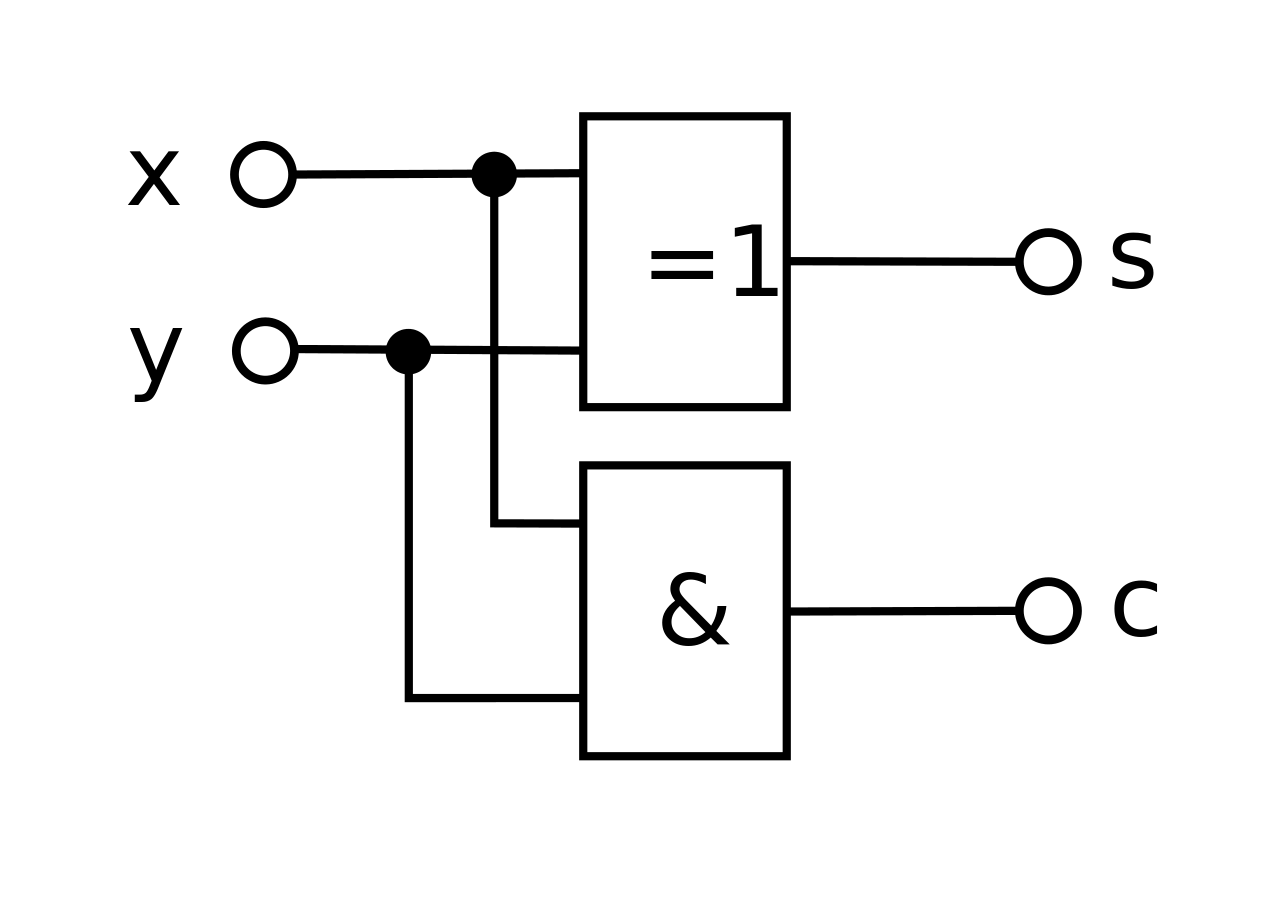
\includegraphics[scale=.2]{Bilder/HalbaddiererAlternativ.png}
	\end{center}
\end{minipage}
\hspace{1cm}
\begin{minipage}[t]{.45\textwidth}
	\begin{center}
		Halbaddierer Schaltsymbol:
		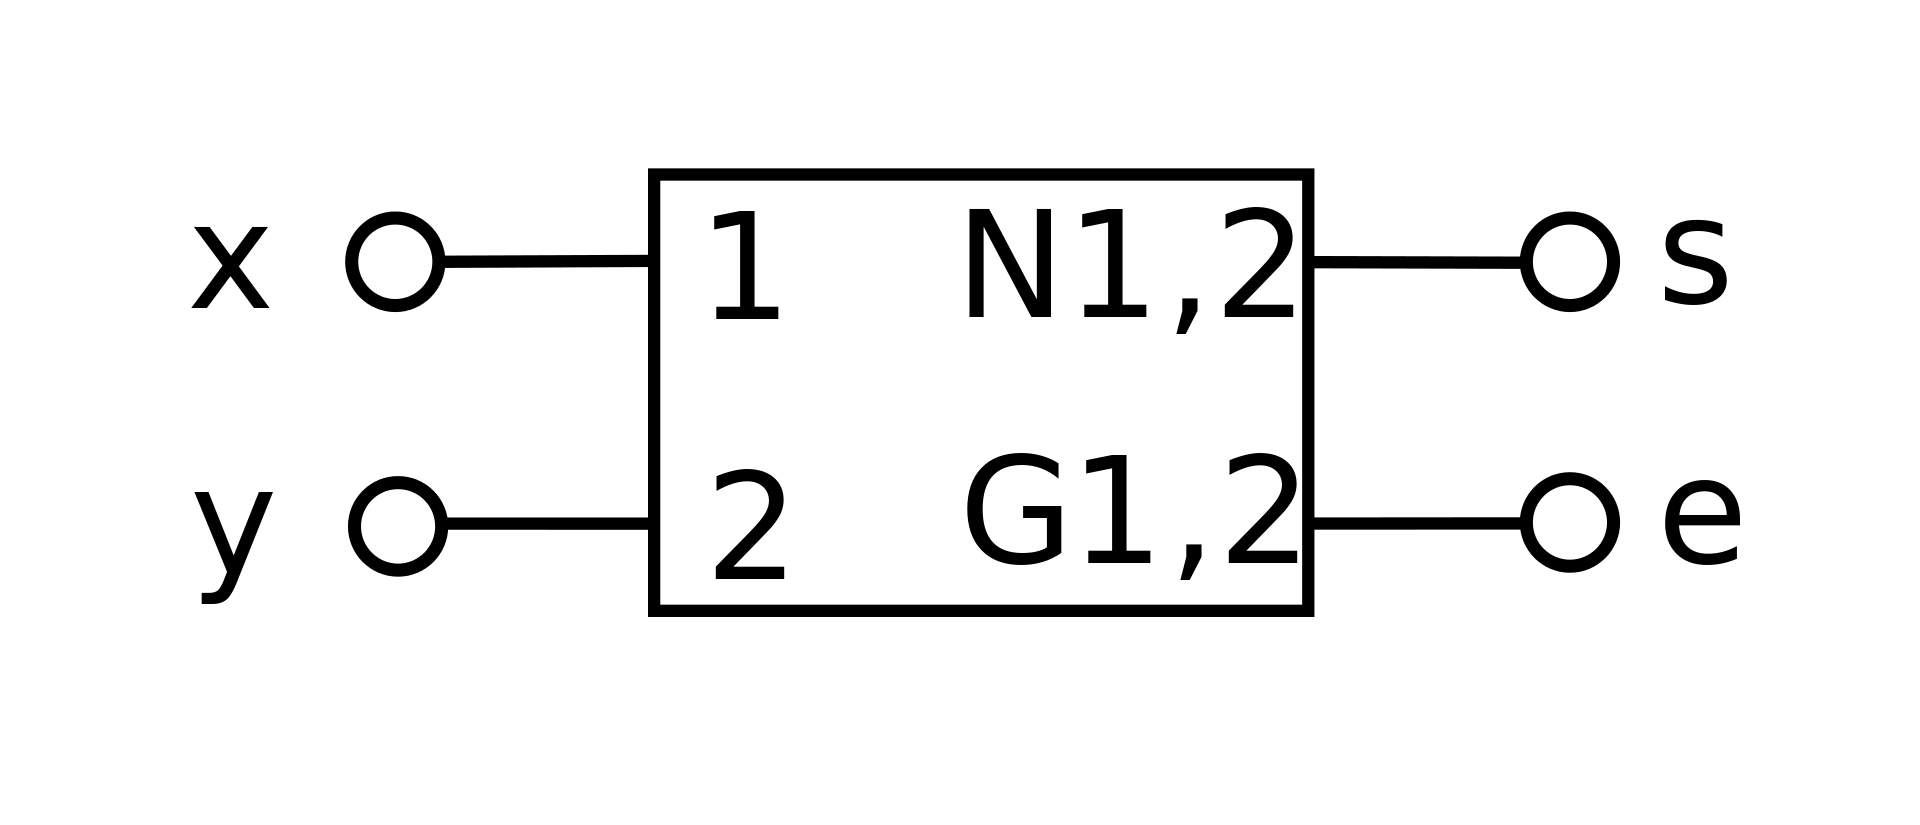
\includegraphics[scale=.13]{Bilder/HalbaddiererSymbol.png}
	\end{center}
\end{minipage}
\par\noindent\rule{\textwidth}{0.4pt}
\vspace{.5cm}
\begin{minipage}[t]{.45\textwidth}
	\begin{center}
		Volladdierer aus zwei Halbaddern und einem OR:
		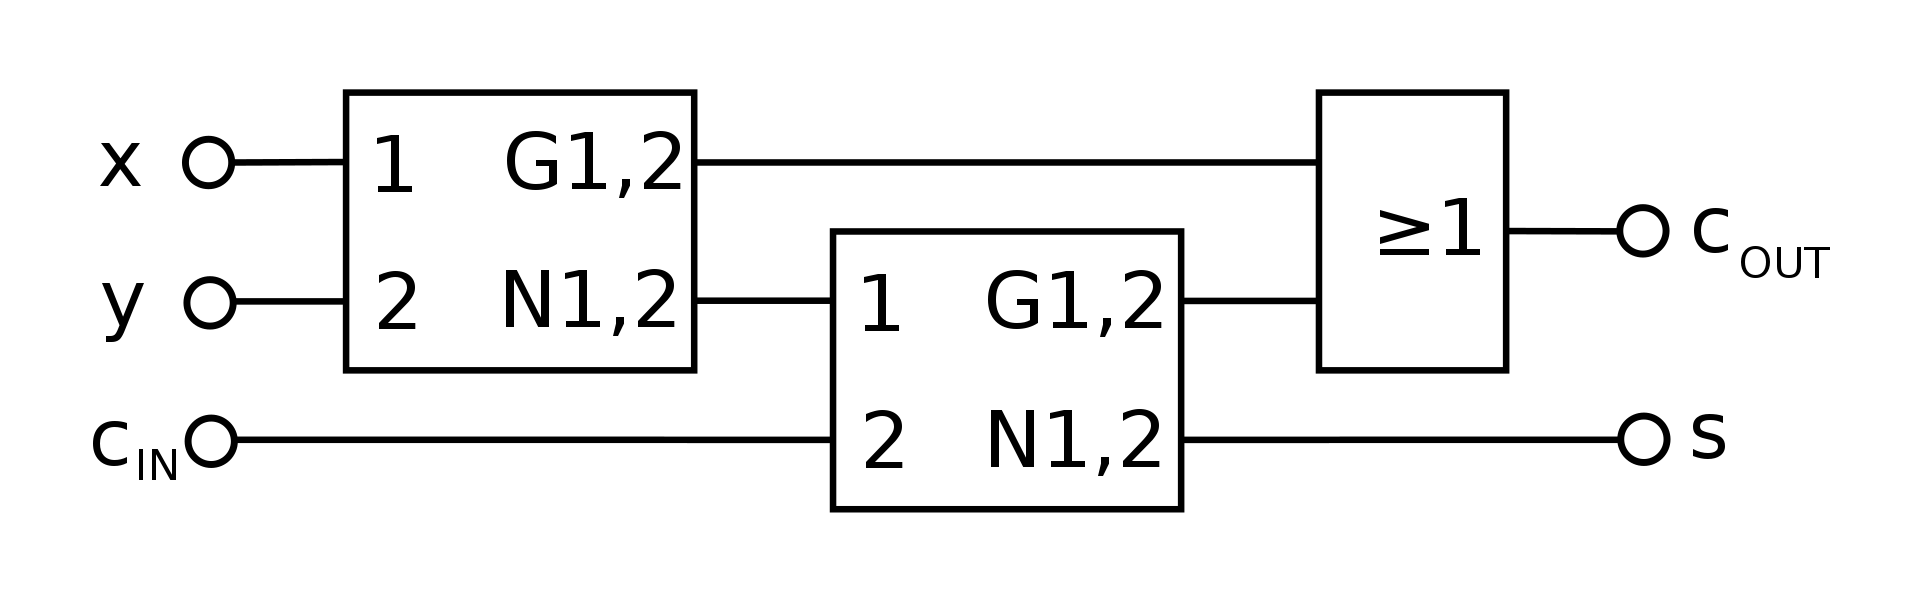
\includegraphics[scale=.13]{Bilder/VolladiererAlternativ.png}
	\end{center}
\end{minipage}
\hspace{1cm}
\begin{minipage}[t]{.45\textwidth}
	\begin{center}
		Volladdierer Schaltsymbol:
		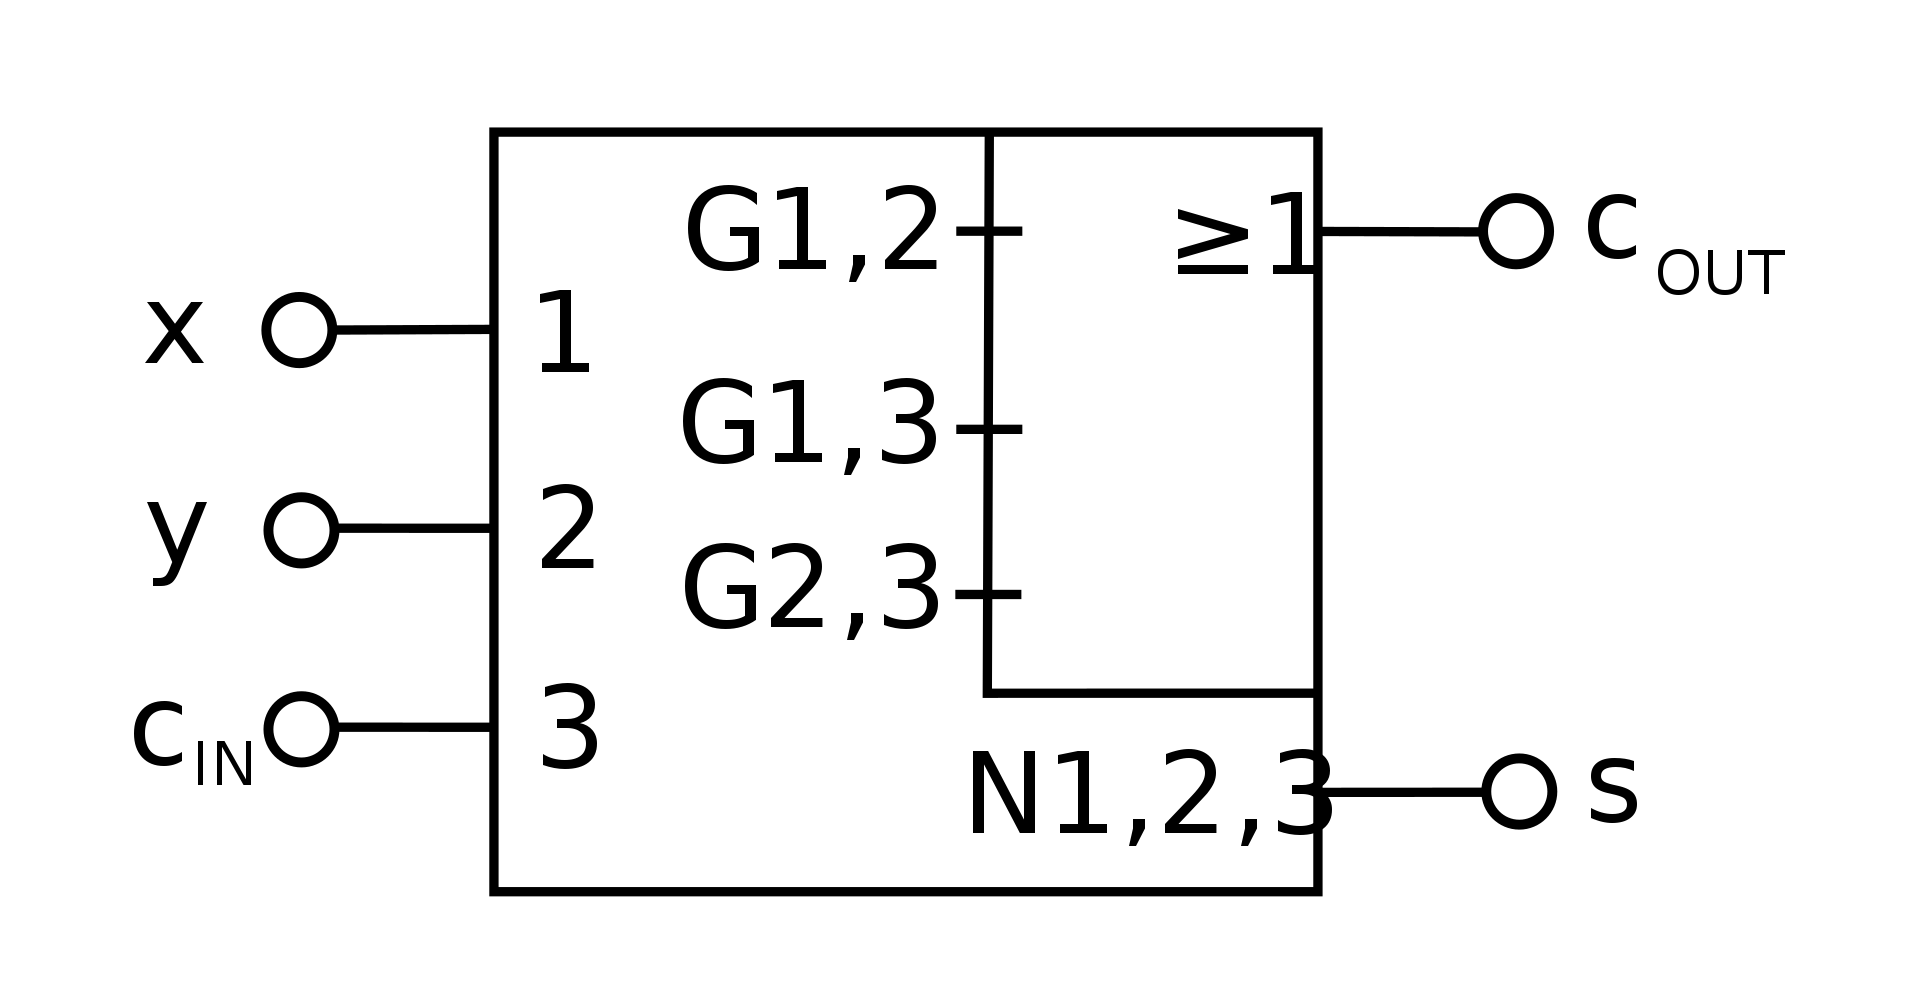
\includegraphics[scale=.13]{Bilder/VolladdiererSymbol.png}
	\end{center}
\end{minipage}

\subsection{Subtrahierschaltungen}
    Subtrahierschaltungen lassen sich aufteilen in Halb- und Vollsubtrahierer. Diese unterscheiden sich in der Größe der Subtrahenden.

%Vorbereitung für die Grafiken. Man muss nur noch eintragen.    
%    
%\par\noindent\rule{\textwidth}{0.4pt}
%\vspace{.5cm}
%\begin{minipage}[t]{.45\textwidth}
%	\begin{center}
%		
%		\includegraphics[scale=.2]{Bilder/}
%	\end{center}
%\end{minipage}
%\hspace{1cm}
%\begin{minipage}[t]{.45\textwidth}
%	\begin{center}
%		
%		\includegraphics[scale=.13]{Bilder/}
%	\end{center}
%\end{minipage}
%\par\noindent\rule{\textwidth}{0.4pt}
%\vspace{.5cm}
%\begin{minipage}[t]{.45\textwidth}
%	\begin{center}
%		
%		\includegraphics[scale=.13]{Bilder/}
%	\end{center}
%\end{minipage}
%\hspace{1cm}
%\begin{minipage}[t]{.45\textwidth}
%	\begin{center}
%		
%		\includegraphics[scale=.13]{Bilder/}
%	\end{center}
%\end{minipage}

\subsection{Schieberegister}
    Mehrere in Reihe geschaltete Flipflops schieben ihren Speicherinhalt bei jedem Arbeitstakt um ein Flipflop weiter – anschaulich gesehen ähnlich einer Eimerkette. Die Anzahl der im Register vorhandenen Speicherplätze ist konstant.
    \begin{center}
        \begin{tikzpicture}
            \draw[black,very thick](-0.5,0)--(-0.5,0.5)--(-2,0.5)--(-2,3)--(2,3)--(2,0.5)--(0.5,0.5)--(0.5,0);
            \draw[black,very thick](-2,-4) rectangle (2,0);
            \draw[black,very thick](-2,1.6)--(-1.7,1.3)--(-2,1);
            \draw[black,very thick](-3,1.3)--(-2,1.3);
            \draw[black,very thick](-3,2.25)--(-2,2.25);
            \draw[black,very thick](-2,-1)--(2,-1);
            \draw[black,very thick](-2,-2)--(2,-2);
            \draw[black,very thick](-2,-3)--(2,-3);
            \draw[black,very thick](2,-0.5)--(2.5,-0.5);
            \draw[black,very thick](2,-1.5)--(2.5,-1.5);
            \draw[black,very thick](2,-2.5)--(2.5,-2.5);
            \draw[black,very thick](2,-3.5)--(2.5,-3.5);
            \node at (3,-0.5){Q1};
            \node at (3,-1.5){Q2};
            \node at (3,-2.5){Q3};
            \node at (3,-3.5){Q4};
            \node at (-3.5,1.3){E};
            \node at (-3.5,2.25){T};
            \node at (0,2.5){SRG4};
        \end{tikzpicture}
    \end{center}

\subsection{Entprellen von Signalen}
    Ein Signal ist prellfrei, wenn das Signal sauber als Ein- oder Ausschaltsignal entziffert werden kann.
    Hier ein Beispiel zum Entprellen eines Tasters:
    \begin{center}
        \begin{tikzpicture}
            \draw[black,very thick, dotted](0,-2) rectangle (4,2);
            \draw[black,very thick](-4,1.3)--(-4,0.5)--(-3.5,0.5)--(-2.5,0.8);
            \draw[black,very thick] (-4,1.5) circle (0.2);
            \draw[black,very thick](-3,0.6)--(-3,2);
            \draw[black,very thick](-3.6,2)--(-2.4,2);
            \node at (-3,2.3){Taster};
            \draw[black,very thick](-2.7,0.6)--(-2.7,1)--(2.1,1);
            \draw[black,very thick] (2.3,1) circle (0.2);
            \draw[black,very thick](2.5,0) rectangle (3.5,1.5);
            \node at (1.7,2.3){digitale Schaltung:};
            \node at (3,0.75){\textbf{\&}};
            \draw[black,very thick](-2.7,0.3)--(-2.7,-0.1)--(0.5,-0.1);
            \node at (-1,0.3){e2};
            \node at (-1,1.3){e1};
            \draw[black,very thick](0.5,-1)rectangle(1.5,0.5);
            \node at (1,-0.25){\textbf{$\geq 1$}};
            \draw[black,very thick](1.5,-0.25)--(2,-0.25)--(2,0.5)--(2.5,0.5);
            \draw[black,very thick](0.5,-0.4)--(0.25,-0.4)--(0.25,-1.5)--(3.75,-1.5)--(3.75,0.75);
            \draw[black,very thick](3.5,0.75)--(4.5,0.75);
            \node at (4.75,0.75){Q};
            \node at (-5,1.5){Vc=5V};
            \draw[black,very thick](-1.5,-0.1)--(-1.5,-1);
            \draw[black,very thick](-2,1)--(-2,-1);
            \draw[black,very thick](-2.2,-1) rectangle (-1.8,-1.75);
            \draw[black,very thick](-1.7,-1) rectangle (-1.3,-1.75);
            \draw[black,very thick](-1.5,-1.75)--(-1.5,-2);
            \draw[black,very thick](-2,-1.75)--(-2,-2);
            \draw[black,very thick](-2.5,-2)--(-1,-2);
            \node at (-2.5,-1.375){R1};
            \node at (-1,-1.375){R2};
            \node at (-3,-2){GND};
        \end{tikzpicture}
    \end{center}
    Die Wiederstände R1 und R2 dienen zum Entladen der Leitungen e1 und e2 nach Umschalten des Tasters. Nur die markierte digitale Schaltung dient zum Entprellen des Tasters. Oft wird aber auch mit Flip Flops ein Signal entprellt.

\section{Mirkocontroller}

\subsection{Aufbau}
    Ein Mirkocontroller besteht aus CPU, RAM, internen und externen Speichern, Interrupts, Timern und Ports.
    Wir beschäftigen uns hier ausschließlich mit dem 8051-Controller.
    \begin{table}[h]
        \centering
        \begin{tabularx}{17cm}{|X|X|}
            \hline
            \textbf{Variante} & \textbf{Größe}\\
            \hline
            Port X & Byte\\
            \hline
            Port X.Y & Bit\\
            \hline
            Akku & Byte\\
            \hline
            Register $\text{R}_{\text{n}}$ & Byte\\
            \hline
        \end{tabularx}
    \end{table}
    Außerdem gibt es noch Datenpointer, welche ein gesamtes Byte aus einer Tabelle in den Akku laden können.
    Interrupts sind Prozesse, welche ganz nach oben auf den Stack gelegt werden und dann direkt abgearbeitet werden. Sie unterbrechen damit eine Abfolge von Prozessen da ihre Priorität höher ist. Der Stack ist ein Stapel an Prozessen, welcher von der CPU abgearbeitet werden muss.

\section{Assembler}
    Eine Assemblersprache, kurz auch Assembler genannt, ist eine Programmiersprache, die auf den Befehlsvorrat eines
    bestimmten Computertyps ausgerichtet ist. Sie ist die letzte/tiefste Sprache vor der Maschienensprache. Alle Hochsprachen basieren auf Assembler oder C.

\subsection{Wichtige Befehle}

\subsection{Adressierungsarten bei Mikrocontroller}

\subsection{Datenpointer}
    Der Datenpointer kann mithilfe des Akkus auf eine 1 Byte-große Zeile in einer Tabelle verweisen und diese in den Akku laden.
    Vor der Benutzung eines Datenpointers, muss man diesen zuerst initialisieren. Hierzu schreibt man:
    \begin{flushleft}
        \textcolor{blue}{MOV DPTR, \#tabelle}
    \end{flushleft}
    Um nun eine Zeile aus der Tabelle in den Akku zu laden, schreibt man die Nummer der Zeile in den Akku und benutzt den Befehl MOVC:
    \begin{flushleft}
        \textcolor{blue}{MOV A, \#2\newline
        MOVC A, @A+DPTR\newline
        MOV A, P2 ;Speichert Zeile in Port 2}
    \end{flushleft}
    Die Tabelle muss folgendermaßen gestaltet werden:
    \begin{flushleft}
        \textcolor{blue}{tabelle:\newline
        db 0101 0111b\newline
        db 0001 1010b\newline
        db 1010 1000b\newline
        ...}
    \end{flushleft}
    'db' steht für define Byte und 'b' für Binär. Statt binär kann man natürlich auch 'h' für Hexadezimal oder 'd' für Dezimal nehmen.
    Wichtig ist außerdem, dass wenn bei Hexadezimal-Darstellung die erste Ziffer einer Zeile mit einem Buchstaben beginnt, eine 0 davor muss.\newline 
    Beispiel: \textit{db A2h} muss als \textit{db 0A2h} geschrieben werden.
    
\subsection{Zeitschleife erstellen ohne Timer}
    Aufgrund Covid-19 ist der Timer kein Bestandteil des diesjährigen Abiturs, weshalb wir Wartezeiten nur mit Schleifen erstellen können. Hierbei verwenden wir Register. Man setzt die 8-Bit Register auf eine Zahl und bildet mit mindestens 2 Registern eine Schleife. Zuerst wird der Wert des inneren Registers immer um 1 reduziert, bis es 0 ist, dann wird das äußere Register um 1 reduziert und das Innere Register beginnt von neu. Hierbei wird je nach Geschwindigkeit des Mikrocontrollers eine Wartezeit erzeugt.
    \begin{center}
        \begin{tikzpicture}
            \draw [black,very thick](0, 2) ellipse (2 and 0.7);
            \node at (0,2){Zeitschleife};
            \draw [black,very thick](0,1.3)--(0,0.5);
            \draw [black,very thick](-2,0.5) rectangle (2,-0.5);
            \node at (0,0){$\text{R}_{\text{1}}$=255d};
            \draw [black,very thick](0,-1)--(0,-0.5);
            \draw [black,very thick](-2,-1) rectangle (2,-2);
            \node at (0,-1.5){$\text{R}_{\text{2}}$=220d};
            \draw [black,very thick](0,-2)--(0,-2.5);
            \draw [black,very thick](-2,-2.5) rectangle (2,-3.5);
            \node at (0,-3){$\text{R}_{\text{2}}$=$\text{R}_{\text{2}}$-1};
            \draw [black,very thick](0,-3.5)--(0,-4)--(2,-5)--(0,-6)--(-2,-5)--(0,-4);
            \draw [black,very thick](2,-5)--(4,-5)--(4,-2.25);
            \draw [black,very thick, ->](4,-2.25)--(0,-2.25);
            \node at (0,-5){$\text{R}_{\text{2}}$=0?};
            \node at (3,-4.75){Nein};
            \draw [black,very thick](0,-6)--(0,-6.5);
            \node at (0.25,-6.25){Ja};
            \draw [black,very thick](-2,-6.5) rectangle (2,-7.5);
            \node at (0,-7){$\text{R}_{\text{1}}$=$\text{R}_{\text{1}}$-1};
            \draw [black,very thick](0,-7.5)--(0,-8)--(2,-9)--(0,-10)--(-2,-9)--(0,-8);
            \node at (0,-9){$\text{R}_{\text{1}}$=0?};
            \node at (-3,-8.75){Nein};
            \draw [black,very thick](-2,-9)--(-4,-9)--(-4,-0.75);
            \draw [black,very thick, ->](-4,-0.75)--(0,-0.75);
            \draw [black,very thick](0,-10)--(0,-10.5);
            \node at (0.25,-10.25){Ja};
            \draw [black,very thick](0,-11.2) ellipse (2 and 0.7);
            \node at (0,-11.2){Ende};
        \end{tikzpicture}
    \end{center}
    
\subsection{Zeitberechnung mit der Näherungsformel}
    Die Formel lautet:
    \begin{center}
        Zeit = Maschienenzyklengeschwindigkeit des Mikrocontrollers * Wert R1 * Wert R2 * Maschienenzyklen für DJNZ Befehl
    \end{center}
    \textbf{Beispiel:}\newline
    R1=255 \& R2=220 \& Geschw. des Mikrocontrollers=1MZ \& DJNZ-Befehl=2MZ\newline
    \begin{center}
        $\text{t} = 2*255*220 = 112200\text{\textmu s} = 112,2\text{ms} = 0,1122\text{s}$    
    \end{center}
    Wenn man die ganz genaue Zeit eines Programmes berechnen will, muss man natürlich noch alle Initialisierungsbefehle, usw. hinzuaddieren.
    
\subsection{Interrupt}
    In der Informatik versteht man unter einem Interrupt eine kurzfristige Unterbrechung der normalen Programmausführung, um einen, in der Regel kurzen, aber zeitlich kritischen, Vorgang abzuarbeiten. Das Program, welches nach dem Interrupt ausgeführt wird nennt man Interrupt Service Routine(ISR).
    Um den Interrupt verwenden zu können, muss man ihn zuerst initialisieren. Dazu muss man in der Formelsammlung des Mirkocontrollers nachschauen, welche Ports Interrupt-fähig sind. An diesen Ports kann man nun seinen Interrupt aktivieren und Einstellen wann er reagieren soll.\newline
    Eine mögliche Initialisierung könnte folgendermaßen aussehen:
    \begin{table}[h]
        \centering
        \begin{tabularx}{5cm}{XX}
            Init: & SETB IT0\\
            &SETB EX0\\
            &SETB EAL\\
        \end{tabularx}
    \end{table}
    \vspace{1cm}
    \newline Um die ISR zu schreiben, muss man die Einsprung Adresse des Interrupts finden.\newline
    Dies sieht dann folgendermaßen aus:
    \begin{table}[h]
        \centering
        \begin{tabularx}{6cm}{XX}
            \textbf{ORG 0003h:} & \\
            marke0: & ...\\
            & ...\\
        \end{tabularx}
    \end{table}

\section{Objektorientierte Programmierung}

\subsection{Grundverständnis}
    Die objektorientierte Programmierung ist ein auf dem Konzept der Objektorientierung basierendes
    Programmierparadigma. Die Grundidee besteht darin, die Architektur einer Software an den Grundstrukturen desjenigen
    Bereichs der Wirklichkeit auszurichten, der die gegebene Anwendung betrifft.

\subsection{Klassen}
    Unter einer Klasse versteht man in der objektorientierten Programmierung ein abstraktes Modell bzw. einen Bauplan für eine Reihe von ähnlichen Objekten. Die Klasse dient als Bauplan für die Abbildung von realen Objekten in Softwareobjekte und beschreibt Attribute und Methoden der Objekte.

\subsection{Objekte}
    In den meisten objektorientierten Programmiersprachen wird ein Objekt oder Exemplar (auch Instanz genannt) aus einer Klasse erzeugt, mittels Konstruktion (siehe auch Konstruktoren und Destruktoren). Diese Instanz besitzt dann zur Laufzeit ihren eigenen Datentyp, eigene Eigenschaften und Methoden. Ein Beispiel für Klassen und Objekte ist ein Mitarbeiter Programm wobei die Klasse ein Formular mit auszufüllenden Daten zu den Mitarbeitern ist und jeder Mitarbeiter ein eigenes Objekt ist, bei dem die Daten eingetragen sind.

\subsection{Datentypen}
    Unter den wichtigen Datentypen in der Hochsprache C\# befinden sich:
    \begin{table}[h]
        \centering
        \begin{tabularx}{17cm}{|X|X|}
            \hline
            int & Integer sind positive oder negative ganze Zahlen\\
            \hline
            double & Kommazahlen und Ganze Zahlen\\
            \hline
            float & 4 Byte große Gleitkommazahl\\
            \hline
            string & Zeichenfolgen/Text\\
            \hline
            bool & Wahr oder falsch, 1 oder 0, binärer Zustand\\
            \hline
            char & einzelner Character\\
            \hline
        \end{tabularx}
    \end{table}

\subsection{Arrays}
    Ein Array/Feld ist in der Informatik eine Datenstruktur-Variante, mit deren Verwendung viele gleichartig strukturierte Daten […] verarbeitet werden sollen. Der Zugriff auf bestimmte Inhalte eines Felds erfolgt mit Hilfe von Indizes, die dessen Position bezeichnen.
    \begin{center}
        \textit{int[] myArray = new int[3];}
    \end{center}
    Ein Array namens \textit{myArray} wurde erstellt und ihm wurden drei Integer-Speicheradressen reserviert.

\subsection{Verebung}
    Wenn Klassen erben, besitzen diese eine abstrakte \textit{Mutterklasse}. Diese vererbt Methoden und Attribute. Für jedes Objekt gibt es nun 2 Objekte. Eines der Mutterklasse und eines der Unterklasse. Ein gutes Beispiel hierfür ist die Mutterklasse Fahrzeug mit ihrer \textit{Kindklasse} PKW.
    Beim Aufrufen des Konstruktors von PKW wird ebenso der Konstruktor der Klasse Fahrzeug aufgerufen.

\subsection{Polymorphie}
\subsubsection{Polymorphie}
    Polymorphie bedeutet, dass ein Bezeichner abhängig von seiner Verwendung, Objekte unterschiedlichen Datentyps annehmen kann. Somit kann man mit einem Verweis/Pointer mehrere Objekte/Datentypen aufrufen.
    Eine Methode ist polymorph, wenn sie in verschiedenen Klassen die gleiche Signatur hat, jedoch erneut implementiert ist.
    Polymorphie wird oft auch als Überladen beschrieben. Ebenso ist das Überladen einer Methode mit unterschiedlichen oder unterschiedlich vielen Parametern Polymorphie.

\subsubsection{Dynamische Polymorphie}
    Man spricht von der dynamischen Polymorphie, wenn Methoden von einer Basisklasse/Mutterklasse abgeleitet und unterschiedlich implementiert werden. Dies wird auch als Überschreiben von Methoden bezeichnet.

\subsection{UML}
    Die Unified Modeling Language, kurz UML, ist eine grafische Modellierungssprache zur Spezifikation, Konstruktion, Dokumentation und Visualisierung von Software-Teilen und anderen Systemen. Sie wird von der Object Management Group entwickelt und ist sowohl von ihr als auch von der ISO genormt.

\subsubsection{Struktogramm}
    Ein Struktogramm wird verwendet um einen Ablauf eines Programmes dar zu stellen.
    \begin{center}
    	\begin{minipage}{.4\textwidth}
        \color{gray}
        public void methode()\{\\
        \hspace*{0.5cm}Anweisung;\\
        \hspace*{0.5cm}for(int i=0; i<=n; i++)\{\\
        \hspace*{1cm}if(Bedingung)\{\\
        \hspace*{1.5cm}Anweisung1;\\
        \hspace*{1cm}\}else\{\\
        \hspace*{1.5cm}Anweisung2;\\
        \hspace*{1cm}\}\\
        \hspace*{0.5cm}\}\\
        \hspace*{0.5cm}Anweisung;\\
        \hspace*{0.5cm}switch(Bedingung)\{\\
        \hspace*{1cm}case Fall1: Anweisung1; break;\\
        \hspace*{1cm}case Fall2: Anweisung2; break;\\
        \hspace*{1cm}case Fall3: Anweisung3; break;\\
        \hspace*{1cm}default: Anweisung4;\\
        \hspace*{0.5cm}\}\\
        \hspace*{0.5cm}Anweisung;\\
        \}\\
    \end{minipage}
    \begin{minipage}{.5\textwidth}
        \begin{center}
            \begin{tikzpicture}
                \node at (1,6.25){\textit{methode()}};
                \draw[black,very thick](0,6) rectangle (8,-6);
                \draw[black,very thick](0,5)--(8,5);
                \draw[black,very thick](0,0)--(8,0);
                \draw[black,very thick](1,0)--(1,4)--(8,4);
                \draw[black,very thick](1,4)--(4.5,1)--(8,4);
                \draw[black,very thick](1,1)--(8,1);
                \draw[black,very thick](4.5,1)--(4.5,0);
                \node at (4.5,3){Bedingung};
                \node at (2.75,1.5){wahr};
                \node at (6.25,1.5){falsch};
                \node at (2.75,0.5){Anweisung1};
                \node at (6.25,0.5){Anweisung2};
                \node at (2.5,4.5){für i:=0 bis n, Schritt: +1};
                \node at (1.4,5.5){Anweisung};
                \draw[black,very thick](0,-1)--(8,-1);
                \draw[black,very thick](0,-1)--(6,-3)--(8,-1);
                \draw[black,very thick](0,-4)--(8,-4);
                \draw[black,very thick](2,-5)--(2,-1.67);
                \draw[black,very thick](4,-5)--(4,-2.35);
                \draw[black,very thick](6,-5)--(6,-3);
                \draw[black,very thick](0,-5)--(8,-5);
                \node at (5.5,-2){Selektor=};
                \node at (1,-3.5){Fall1};
                \node at (3,-3.5){Fall2};
                \node at (5,-3.5){Fall3};
                \node at (7,-3.5){sonst};
                \node at (1,-4.5){Anw.1};
                \node at (3,-4.5){Anw.2};
                \node at (5,-4.5){Anw.3};
                \node at (7,-4.5){Anw.4};
                \node at (1.4,-5.5){Anweisung};
                \node at (1.4,-0.5){Anweisung};
            \end{tikzpicture}
        \end{center}
    \end{minipage}
    \end{center}

\subsubsection{Klassendiagramm}
    Klassendiagramme können vereinfacht und detailliert dargestellt werden. Sie veranschaulichen alle Attribute und Methoden einer Klasse.

\subsubsection{Objektdiagramm}
    Objektdiagramme werden im Bezug zum Klassendiagramm gezeichnet. Sie sind eine Instanz der Klasse und die Attribute sind mit Werten gefüllt.

\subsubsection{Assoziationen}
    Klassendiagramme können außerdem die Assoziationen zwischen verschiedenen Klassen darstellen:

\subsubsection{Polymorphie}
    Polymorphie beschreibt das Erben zwischen Klassen und veranschaulicht dies.

\subsubsection{Vererbungen}
    Vererbungen können außerdem vereinfacht dargestellt werden.

\subsubsection{Sequenzdiagramm}
    Sequenzdiagramme stellen den Ablauf eines Programmes dar. Hierbei sieht man außerdem die Schritte in den verschiedenen Klassen.

\subsubsection{Zustandsdiagramm}
    Beim Zustandsdiagramm kann man herauslesen, wie das Programm in einem gewissen Zustand fortfahren kann. Hierbei wird jeder Zustand aufgezeichnet und alle möglichen Optionen ergänzt.

\section{Datenbanken}
\subsection{Grundverständnis Datenbanken}
    Eine Datenbank, auch Datenbanksystem genannt, ist ein System zur elektronischen Datenverwaltung. Die wesentliche Aufgabe einer Datenbank ist es, große Datenmengen effizient, widerspruchsfrei und dauerhaft zu speichern und benötigte Teilmengen in unterschiedlichen, bedarfsgerechten Darstellungsformen für Benutzer und Anwendungsprogramme bereitzustellen.
    Eine Datenbank besteht aus mehreren Tabellen. Jede Tabelle hat eigene Spalten. Diese Tabellen können zusammenarbeiten und effizient Daten speichern. Daten müssen nicht doppelt oder dreifach gespeichert werden.

\subsection{Verwendung}
    Um Daten dauerhaft, effizeint und widerspruchsfrei zu speichern.

\subsection{Entity-Relationship-Diagramm}
    Das ER-Diagramm gibt einen schnellen und übersichtlichen Überblick über die Tabellen einer Datenbank. Das ER-Diagramm wird zum Beispiel beim Erstellen und Planen einer Datenbank verwendet.
    Bevor man das ER-Diagramm zeichnen will, sollte man sich aber alle Beziehungen der Tabellen ansehen. Treten n:m-Beziehungen auf, müssen diese zuerst aufgelöst werden:\newline
    \textbf{1:1 Beziehung:}
    \begin{center}
        \begin{tikzpicture}
            \draw[black,very thick](-7,-1) rectangle (-3,1);
            \draw[black,very thick](-3,0)--(3,0);
            \draw[black,very thick](3,-1) rectangle (7,1);
            \node at (-2.5,0.5){1};
            \node at (2.5,0.5){1};
            \node at (-5,0){Entität 1};
            \node at (5,0){Entität 2};
        \end{tikzpicture}
    \end{center}

    \textbf{1:n Beziehung:}
    \begin{center}
        \begin{tikzpicture}
            \draw[black,very thick](-7,-1) rectangle (-3,1);
            \draw[black,very thick](-3,0)--(3,0);
            \draw[black,very thick](3,-1) rectangle (7,1);
            \node at (-2.5,0.5){1};
            \node at (2.5,0.5){N};
            \node at (-5,0){Entität 1};
            \node at (5,0){Entität 2};
        \end{tikzpicture}
    \end{center}

    \textbf{n:m Beziehung:}
    \begin{center}
        \begin{tikzpicture}
            \draw[black,very thick](-7,-1) rectangle (-3,1);
            \draw[black,very thick](-3,0)--(3,0);
            \draw[black,very thick](3,-1) rectangle (7,1);
            \node at (-2.5,0.5){N};
            \node at (2.5,0.5){M};
            \node at (-5,0){Entität 1};
            \node at (5,0){Entität 2};
        \end{tikzpicture}
    \end{center}

    \textbf{n:m Beziehung(aufgelöst):}
    \begin{center}
        \begin{tikzpicture}
            \draw[black,very thick](-8,-1) rectangle (-4,1);
            \draw[black,very thick](-4,0)--(-2,0);
            \draw[black,very thick](4,0)--(2,0);
            \draw[black,very thick](4,-1) rectangle (8,1);
            \node at (-3.5,0.5){1};
            \node at (3.5,0.5){1};
            \node at (-2.5,0.5){N};
            \node at (2.5,0.5){M};
            \node at (-6,0){Entität 1};
            \node at (6,0){Entität 2};
            \node at (0,0){Verbindungsentität};
            \draw[black,very thick](-2,-1) rectangle (2,1);
        \end{tikzpicture}
    \end{center}

\subsection{Primärschlüssel}
    Der Primärschlüssel findet sich in jeder Tabelle einer Datenbank. Er ist meist die ID der jeweiligen Einträge, da diese sich nicht doppelt. Mit dem Primär- und Sekundärschlüssel können Tabellen verknüpft werden.
    
\subsection{Sekundärschlüssel}
    Der Sekundärschlüssel ist der Primärschlüssel der jeweils anderen Tabelle. Dieser befindet sich außerdem in der lokalen Tabelle.

\subsection{Realtionsschreibweise}
    Bei der Realtionsschreibweise erkennt man direkt die wichtigsten Informationen und die Spalten einer Datenbank. Hierbei muss deutlich klar gemacht werden, was der Primär- und was der Sekundärschlüssel sind.\newline
    \textbf{Beispiel:}\newline
    Angestellter(\textbf{PerNr}, Name, Vorname, \underline{AbtNr})\newline
    Abteilung(\textbf{AbtNr}, Bezeichnung)\newline
    \vspace{0.2cm}\newline
    Legende:\newline
    \textbf{Fett}=Primärschlüssel, \underline{Unterstrichen}=Sekundärschlüssel
    
\subsection{SQL}
    SQL ist eine Datenbanksprache zur Definition von Datenstrukturen in relationalen Datenbanken sowie zum Bearbeiten und Abfragen von darauf basierenden Datenbeständen.

\subsubsection{SQL Abfragen}
    Um gefilterte Informationen aus Datenbanken zu entnehmen werden SQL-Abfragen geschrieben. Mit diesen kann man mehrere Tabellen verknüpfen und gefiltert nach den gewünschten Daten suchen.\newline
    \vspace{0.5cm}\newline
    \textbf{SELECT Buchungen.BuchungsID, Buchungen.KundenID, \newline
    Kunden.Name FROM Kunden, Buchungen\newline
    WHERE Kunden.KundenID = Buchungen.KundenID\newline
    AND KUNDEN.Name LIKE "Müller"\newline}
    \vspace{0.5cm}\newline
    Mit diesem Befehl werden alle Buchungsnummern, Kundennummern und 
    Kundennamen von Kunden mit dem Namen Müller ausgegeben.\newline
    \vspace{1cm}\newline
    Der Aufbau einer SQL-Abfrage muss folgende Reihenfolge einhalten:\newline
    \textbf{SELECT <Spalte>,<Aggregatfunktion>\newline
    FROM <Tabelle>\newline
    WHERE <Bedingung>\newline
    GROUP BY <Spalte>\newline
    HAVING <Aggregatfunktion> <VerglOp> <Wert>\newline
    ORDER BY <Spalte>[ASC|DESC], <Aggregatfunktion>\newline
    LIMIT [start,] anzahl}\newline
    \vspace{1cm}\newline
    Hier einige Befehle:
    \begin{table}[h]
        \centering
        \begin{tabularx}{17cm}{|X|X|}
            \hline
            DISTINCT & Vermeidet doppelte Datensätze(kommt nach SELECT)\\
            \hline
            ASC & Alphabetische/Aufsteigende Sortierung\\
            \hline
            DESC & Absteigende Sortierung\\
            \hline
            SUM() & Summe\\
            \hline
            COUNT() & Anzahl\\
            \hline
            AVG() & Durchschnittlicher Wert\\
            \hline
            MAX() & Höchster Wert\\
            \hline
            MIN() & Kleinster Wert\\
            \hline
        \end{tabularx}
    \end{table}
    \vspace{0.5cm}\newline
    Beispiel:\newline
    \textbf{SELECT fahrradtypen.Typbezeichnung, SUM(DATEDIFF(bis, von) * Tagesmietpreis) AS "Mieteinnahmen"\newline
    FROM fahrraeder, fahrradtypen, vermietungen\newline
    WHERE fahrraeder.FahrradNr = vermietungen.FahrradNr\newline
    AND fahrradtypen.TypNr = vermietungen.TypNr\newline
    GROUP BY fahrradtypen.Typbezeichnung\newline
    HAVING SUM(DATEDIFF(bis, von) * Tagesmietpreis) >= 1000}\newline
    \vspace{0.5cm}\newline
    Mit diesem Befehl werden alle Mieteinnahmen und Fahrradtyp ausgegeben bei denen die Mieteinnahmen größer als 1000€ sind.

\section{Fachsprache}
\subsection{Fachwörter}
    \begin{table}[h]
        \renewcommand{\arraystretch}{2}
        \begin{tabularx}{17cm}{|l|X|}
            \hline
            Fachbegriff&Erklärung\\
            \hline
            \hline
            Algorithmus&Eine genau definierte Handlungsvorschrift zur Lösung von Problemen in endlich vielen Schritten\\
            \hline
            Attribut&Eigenschaft einer Klasse\\
            \hline
            ASCII&American Standard Code for Information Interchange\\
            \hline
            ARP&Adress Resolution Protocol\\
            \hline
            BCD-Code&Binary Coded Decimal (dualkodierte Dezimalziffer)\\
            \hline
            Client-Server Netz&Ein Client-Server Netz besteht zwischen einem Server und einem Computer. Der Server bietet dem Client verschiedene Dienste an, der Client kann Dienste vom Server anfordern.\\
            \hline
            CRC / FCS& Cyclic Redundancy Check / Frame Check Sequence\\
            \hline
            CSMA/CD&Carrier Sense Multiple Access / Collision Detection\\
            \hline
            Geheimnisprinzip&Lesen oder Schreiben der Attributwerte eines Objekts nur durch Operation möglich\\
            \hline
            Kapselung&Attribute sind durch Operationen von der Außenwelt abgeschlossen (Attribute private, Operationen public)\\
            \hline
            Klasse&Beschreibt Gemeinsamkeiten einer Menge gleichartiger Objekte\\
            \hline
            Klassenattribut&Ein Attributwert für alle Objekte der Klasse\\
            \hline
            MAC Adresse& Media Access Control Adresse\\
            \hline
            MTU&Maximum Transmission Unit (Nutzdatenblock Ethernet Frame)\\
            \hline
            Objekt&Gegenstand der Programmierung (materieller Gegensand, Organisationseinheit, Begriff, Aspekt eines Systems)\\
            \hline
            OUI&Organizationally Unique Identifier\\
            \hline
            OSI (Modell)&Open Systems Interconnedtion (Modell)\\
            \hline
        \end{tabularx}
    \end{table}
    \begin{table}[h]
        \renewcommand{\arraystretch}{2}
        \begin{tabularx}{17cm}{|l|X|}
            \hline
            Fachbegriff&Erklärung\\
            \hline
            \hline
            Peer-to-Peer Netz&Ein Peer-to-Peer Netz besteht aus zwei oder mehreren gleichberechtigten Systemen.\\
            \hline
            Padding&Füllbits zum Auffüllen von Segmenten, in denen der Datenanteil nicht die Mindestgröße ausfüllt.\\
            \hline
            Redundanz&Beschreibt diejenigen Informationen oder Daten, die in einer Informationsquelle mehrfach vorhanden sind. Eine Informationseinheit ist dann redundant, wenn sie ohne Informationsverlust weggelassen werden kann.\\
            \hline
            RTD&Round Trip Delay\\
            \hline
            RTT&Round Trip Time\\
            \hline
            SFD / SOF& Start Frame Delimiter / Start of Frame\\
            \hline
            Virtuelle Kommunikation&Beschreibt die Kommunikation der zwei Systeme auf der entsprechenden Ebene über einheitliche Sprache bzw. Protokolle\\
            \hline
        \end{tabularx}
    \end{table}

\subsection{Typfeld Kennungen}
    \begin{table}[h]
        \centering
        \renewcommand{\arraystretch}{2}
        \begin{tabularx}{17cm}{|l|X|}
            \hline
            0x0800&IPv4 Internet Protocol, Version 4\\
            \hline
            0x0806&ARP Adress Resolution Protocol\\
            \hline
            0x0842&WoL Wake on Lan\\
            \hline
            0x8035&RARP Reverse Adress Resolution Protocol\\
            \hline
            0x809B&EtherTalk Appletalk\\
            \hline
            0x80F3&AARP Appletalk Adress Resolution Protocol\\
            \hline
            0x8100&VLAN Tag\\
            \hline
            0x8137&Novell IPX\\
            \hline
            0x8138&Novell\\
            \hline
            0x86DD&IPv6 Internet Protocol, Version 6\\
            \hline
            0x8863&PPPoE Discovery\\
            \hline
            0x8864&PPPoE Session\\
            \hline
            0x8870&Jumbo Frames\\
            \hline
            0x8892&Echtzeit-Ethernet PROFINET\\
            \hline
            0x88A2&ATA over Ethernet Coraid AoE\\
            \hline
            0x88A4&EtherCAT Echtzeit-Ethernet\\
            \hline
            0x88A8&Provider Bridging\\
            \hline
            0x88AB&Echtzeit-Ethernet POWERLINK\\
            \hline
            0x88CD&Echtzeit-Ethernet SERCOS III\\
            \hline
            0x8906&Fibre Channel over Ethernet\\
            \hline
            0x8914&FCoE Initialization Protocol FIP\\
            \hline
        \end{tabularx}
    \end{table}

\section{Epilog}
    \noindent
    Diese Zusammenfassung wurde erstellt und geteilt von \textit{Robin Rausch} und \textit{Jannis Müller}. Für Falschaussagen oder Fehlinformationen übernehmen die Autoren keinerlei Gewähr. Es ist empfehlenswert, sich selbst mit den Inhalten vertraut zu machen und die hier dargestellten Inhalte gegebenenfalls zu korrigieren. Bei Fragen oder inhaltlichen Fehlern kontaktieren sie bitte umgehend einen der Autoren und weisen auf die von Ihnen festgestellten Mängel hin. 
    
\subsection{Literatur}
Fachwissen sowie einige Inhalte wurden übernommen aus:\newline
\textit{Informatik und Informationstechnik - für Gymnasien und höhere Bildungsgänge im beruflichen Schulwesen (3. Auflage)} verlegt von \textit{Europa Lehrmittel}. 

\end{document}